\documentclass{FastFyp}
\usepackage{float}
\usepackage{tabularx}
\usepackage{longtable}
\usepackage{multirow}
\usepackage{xltabular}
\usepackage{array}
\usepackage{makecell}
\usepackage{graphicx}
\usepackage{subcaption}
\newcolumntype{Y}[1]{>{\hsize=#1\hsize\raggedright\arraybackslash}X}
\begin{document}
\newcommand{\supervisor}{Mr Zeeshan Nazar}
\newcommand{\university}{National University of Computer and Emerging Sciences, Lahore}
\newcommand{\fyptitle}{Silent Signals}
\newcommand{\degree}{BS}
\newcommand{\Studentone}{Ushna Dar     23L-0529    BS(CS)} 
\newcommand{\Studenttwo}{Mawahid Abbas     23L-0613    BS(CS)}
\newcommand{\Studentthree}{Abad Hussain     21L-1827    BS(CS)}
\date{\today}
\renewcommand{\contentsname}{Table of Contents}

\makeatletter
    \begin{titlepage}
        
\includegraphics[width=0.2\linewidth]{Figures/nulogo.png}\hfill
        
\includegraphics[width=0.2\linewidth]{Figures/fast.png}\\
        \begin{center} 
            {\large\bfseries \university}\\[7ex]
            
\includegraphics[width=0.4\linewidth]{Figures/fastlogo.png}\\[8ex]
            {\huge \bfseries  \fyptitle }\\[10ex] 
            {\Studentone}\\{\Studenttwo}\\{\Studentthree}\\[4ex] 
            {Supervisor: \supervisor} \\ [10ex]
            {Final Year Project}\\
            {\large \@date}
        \end{center}
    \end{titlepage}    
\makeatother
\frontmatter

\newpage \thispagestyle{empty} \mbox{} \newpage %Aatira

\pagestyle{empty}  %Aatira
\section*{\begin{center}{Anti-Plagiarism Declaration} \end{center}} %Aatira
This is to declare that the above publication was produced under the:
\begin{flushleft}
\bf Title: \fyptitle
\end{flushleft}

is the sole contribution of the author(s), and no part hereof has been reproduced as it is the basis (cut and paste) that can be considered Plagiarism. All referenced parts have been used to argue the idea and cited properly. I/We will be responsible and liable for any consequence if a violation of this declaration is determined.
\\[4ex]
%% FYPTODO add the date and your names here
Date: ..........................

\begin{flushright}
Name: ..........................
\\[3ex]
Signature: ..........................
\\[6ex]
Name: ..........................
\\[3ex]
Signature: ..........................
\\[6ex]
Name: ..........................
\\[3ex]
Signature: ..........................

\end{flushright} 

\vspace{5 cm} %Aatira
 
\hrule %Aatira

\section*{Author's Declaration}
This states Authors’ declaration that the work presented in the report is their own, and has not been submitted/presented previously to any other institution or organization.
\pagebreak
\section*{Abstract}
People with hearing and speech impairments face a daily communication barrier in classrooms,
hospitals, banks and workplaces, where trained interpreters are rarely available and
conventional speech recognition is of little help because it depends entirely on an audio signal
that the user may not be able to produce or perceive. This project proposes Silent Signals, an
ML-based communication aid that removes this dependence on audio by recognizing speech
visually. The main module is a lip-reading system. It takes either a recorded video or a live
webcam feed of someone’s face and turns their lip movements into on-screen text using a deep
learning model. It works in English and shows a confidence score for each word. It also uses a
language model to clean up the predicted sentences, detects facial expressions for emotional
context, keeps a conversation history, and has an emergency mode that can alert a registered
guardian. The goal is one simple, affordable tool that actually lets people have real two-way
conversations.
\pagebreak 

\section*{Executive Summary}
More than 1.5 billion people worldwide live with some degree of hearing loss, and the World Health Organization projects that this figure will rise to nearly 2.5 billion by 2050 \cite{who2021}. In Pakistan the situation is more difficult because trained sign language interpreters are scarce, and aids such as cochlear implants and speech generating devices are too expensive for most families. A student in a lecture or a patient describing symptoms to a doctor therefore usually depends on whichever relative happens to be present. Existing technology covers only part of the problem. Automatic speech recognition works well on clear audio, but it is of no use to a person who cannot produce clear speech, and it becomes unreliable in the noisy places where help is needed most. Sign language is widely used in the deaf community, but most people outside it do not understand it, so the burden of translation falls back on the user. Schools, hospitals and banks currently have no affordable way to serve these customers directly, which limits access to education, healthcare and financial services.

Silent Signals is a mobile app that allows a person with a hearing or speech impairment to hold a normal two-way conversation without an interpreter and without special hardware. It runs on any device with a camera, such as a laptop or a phone, which keeps the cost of adoption low for both individuals and institutions. The user mouths words in front of the camera, and the system converts their lip movements into text on the screen. A user who communicates through sign language can use the same interface, and the system renders their signs as text as well. The recognized text can then be read aloud so that a hearing person can follow the conversation and reply naturally. A noise suppression component keeps the spoken reply clear in a busy room. Because the main input is visual, the platform continues to work in environments such as hospitals, banks and crowded classrooms, where audio based tools often fail. The system supports English and is designed for everyday situations.

The app includes several features that make it reliable and practical for daily use. Each recognized word is shown with a confidence score, and uncertain words are highlighted so that the user can correct them before they are spoken. A language model fixes spelling and grammar errors in the predicted sentences, for example turning ``I ant watr'' into ``I want water''. Facial expression detection adds emotional context, which helps the listener understand how something is meant. An emergency mode offers one click phrases such as ``I need help'' and sends an automatic alert to a registered guardian or family member, which gives families peace of mind. Users can review earlier conversations in a history with date and time, and a personal profile keeps their activity in one place. Accessibility options such as large text, dark mode and high contrast modes make the interface usable for people with different needs. A performance dashboard shows accuracy, processing time and the number of words recognized, which helps administrators monitor quality.

The project covers the complete development cycle, including data collection, model training, a backend service that hosts the models, a user facing application, integration, testing and deployment. The lip reading model is trained on the Lip Reading in the Wild (LRW) dataset \cite{ref:Chung:2016}, building on earlier work that showed end to end sentence level lip reading to be feasible \cite{assael2016lipnet}. For institutions, the main benefit is a low cost way to serve customers with hearing or speech impairments without hiring interpreters or buying specialised devices. For users, the benefits are independence, safer communication in emergencies and better access to public services. For hearing people, the benefit is that they can communicate naturally without knowing sign language. In conclusion, Silent Signals shows that visual speech recognition, combined with sign language recognition, speech synthesis and noise suppression, can be offered as one affordable product that makes everyday services more inclusive. 
\pagebreak


\pagestyle{fancy} %Aatira
\tableofcontents

\clearpage
\phantomsection
\addcontentsline{toc}{chapter}{List of Figures}
\listoffigures

\clearpage
\phantomsection
\addcontentsline{toc}{chapter}{List of Tables}
\listoftables

\mainmatter


\chapter{Introduction}
Speech is the primary way in which people exchange information, and almost every public service is designed on the assumption that the person using it can both hear and speak. For a large part of the world's population this assumption does not hold. The World Health Organization reports that more than 1.5 billion people live with some degree of hearing loss and projects that the number will rise to nearly 2.5 billion by 2050 \cite{who2021}. People with hearing or speech impairments face a daily communication barrier in classrooms, hospitals, banks and workplaces, where a trained interpreter is rarely available. In Pakistan the barrier is made worse by a shortage of trained sign language interpreters and by the high cost of aids and treatments such as cochlear implants and speech generating devices, which places them beyond the reach of most families. As a result, a student in a lecture, or a patient describing symptoms to a doctor, is usually left dependent on whichever relative happens to be present. This dependence limits privacy, independence and access to basic services.

Technology has addressed only part of this problem. Automatic speech recognition systems of the kind built into modern phones are highly accurate, but they work on an audio signal. They are therefore of no use to a person who cannot produce clear speech, and they become unreliable in noisy environments such as hospitals, banks and crowded classrooms, which are exactly the places where assistance is needed most. Visual speech recognition, also known as lip reading, offers an alternative because it recognizes speech from the movement of the lips and does not need audio at all. LipNet showed that end-to-end sentence level lip reading is possible on the GRID corpus \cite{assael2016lipnet,cooke2006grid}, and later audio-visual models reported word error rates competitive with audio-only systems on large scale data \cite{ref:Afouras:2018}. Sign language is another important channel and is widely used within the deaf community, but it is not understood by many people outside it, so the burden of translation is pushed back onto the user \cite{koller2016deepsign}.

Silent Signals is a machine learning based communication aid that brings these channels together in one product. Its main module is a lip-reading system that takes a recorded video or a live webcam feed, locates the mouth region using face landmark detection \cite{lugaresi2019mediapipe}, and passes the resulting frame sequence to a spatio-temporal deep learning network that outputs English text. A sign language module uses hand and body landmark tracking to render signs as the same on-screen text, so that both groups of users are served through one interface. A text-to-speech module reads the recognized text aloud so that the conversation can flow in both directions, and a sound optimization module applies deep learning based noise suppression so that the spoken reply stays intelligible in a noisy room \cite{valin2018hybrid}. Supporting features include a confidence score for each word, language model based sentence correction, facial expression detection, conversation history and an emergency mode that alerts a registered guardian. The goal is a single, affordable tool that needs no interpreter and no special hardware.

\section{Purpose of this Document}
\textbf{}
This document describes the complete development of Silent Signals, from the background research to the design, implementation, testing and evaluation of the system. It explains the problem that the project addresses, reviews related work in lip reading, sign language recognition, speech synthesis and speech enhancement, and then presents our own approach and how it differs from existing work. The system is delivered as an application backed by a service that hosts the machine learning models. The lip-reading model is trained on the Lip Reading in the Wild (LRW) dataset \cite{ref:Chung:2016}, the sign language model is trained on a vocabulary of common everyday words and phrases, and the system works in English. The application accepts a recorded video or a live webcam feed, shows the recognized text with a confidence score for each word, corrects the sentence using a language model, and can speak the result aloud. It also keeps a conversation history and provides an emergency mode for quick communication with a registered guardian. The document also records the limitations of the work and the directions for future development.

The main research questions that this project aims to answer are as follows. Can a lip-reading model trained on a controlled dataset be used in a real-time application that runs on an ordinary webcam? Can lip reading and sign language recognition be combined in one interface so that people who rely on different channels can use the same tool? Can confidence scores and language model correction make the recognized text reliable enough to be used in everyday conversations? These questions guide the design decisions and the evaluation described in the later chapters. Answering them matters because a system that is accurate only on recorded clips, or only in a laboratory setting, would not help the people who need it. For this reason the evaluation looks at both recorded video and live webcam input, and at how well the system performs when the background is noisy.

\section{Intended Audience}
This document is intended for our supervisor and the FYP evaluation panel, who will use it to judge the problem definition, the technical approach and the quality of the work carried out. It is written for technical readers such as students, researchers and developers who wish to build a similar system, because it summarizes related work on lip reading, sign language recognition, speech enhancement and speech synthesis and explains our design choices. A third group of readers is made up of the people for whom the system is built, namely people with hearing and speech impairments, their families, and the institutions that serve them, such as schools, hospitals and banks. For these readers the executive summary and the project vision chapter give the most useful overview, while the later chapters can be read for the technical detail. Readers are assumed to have a basic understanding of machine learning.
\section{Definitions, Acronyms, and Abbreviations}
In the interest of clarity, this report uses several acronyms. The following list gives each acronym with its full form.

\textbf{SDG}: Sustainable Development Goal\\
\textbf{FYP:} Final Year Project\\
\textbf{ML}: Machine Learning\\
\textbf{UI}: User Interface\\
\textbf{GPU}: Graphics Processing Units\\
\textbf{TTS}: Text-to-Speech\\
\textbf{GRID}: Audio-Visual Corpus for Speech Perception and Recognition\\
\section{Conclusion}
The rest of this report is organized as follows. Chapter~\ref{ch:vision} presents the project vision, including the problem statement, the goals and objectives, the scope and the sustainable development goal that the project supports. Chapter~\ref{ch:lit} reviews related research in lip reading, sign language recognition and translation, speech recognition, speech synthesis, noise suppression and facial expression detection, and summarizes them in a table. Chapter~\ref{ch:srs} lists the features, the functional and non-functional requirements, the use cases and the hardware and software requirements of the system. Chapter~\ref{ch:approach} describes the proposed approach and the methodology followed to prepare the data and train the models. Chapter~\ref{ch:design} presents the high-level and low-level design of the system, including its architecture and its modules.
%  Chapter~\ref{ch:impl} describes the prototype that has been implemented so far and the plan for test cases. Chapter~\ref{ch:concl} concludes the report with a summary of the work done, the limitations and the plan for FYP-II.

\chapter{Project Vision}
\label{ch:vision}
This chapter presents the vision of Silent Signals. It explains what the system does, the problem that it is built to solve, and the goals and scope that the project follows. It also identifies the sustainable development goals that the work supports, the constraints under which it is developed, the business opportunity that it offers and the stakeholders who are affected by it. The chapter forms the base for the requirements in Chapter~\ref{ch:srs} and the design in Chapter~\ref{ch:design}, because every requirement and every design decision in those chapters can be traced back to a goal or a problem described here. The sections are arranged so that the reader first sees the domain and the problem, then the planned solution and its boundaries, and finally the wider context of sustainability, business and users. Where facts about the problem come from outside sources they are cited, and the remaining statements describe our own plan. The chapter closes with a conclusion that links the vision to the literature review that follows.

\section{Problem Domain Overview}
Silent Signals belongs to the domain of assistive communication technology, which uses machine learning, computer vision and speech processing to help people with hearing or speech impairments communicate with others. The system is a web based application backed by a service that hosts the machine learning models. A user signs in, chooses a mode and points a webcam at their face or hands. In lip-reading mode the system crops the mouth region from each video frame and passes the sequence to a deep learning network that predicts the spoken words without any audio \cite{assael2016lipnet}. In sign language mode it tracks hand and body landmarks \cite{lugaresi2019mediapipe} and recognizes signs from a vocabulary of common everyday words and phrases. Both modes produce the same on-screen text, shown with a confidence score for each word and corrected by a language model before the user confirms it. A text-to-speech module then reads the sentence aloud, with noise suppression keeping the reply clear in a noisy room \cite{valin2018hybrid}. Facial expression detection adds emotional context, while conversation history, user profiles, a performance dashboard and accessibility settings support everyday use. In an emergency, one click sends a predefined phrase and an automatic notification to a registered guardian. The system supports English only and runs on a laptop, desktop or phone with a standard camera.
\section{Problem Statement}
People with hearing or speech impairments cannot take part fully in everyday conversations in classrooms, hospitals, banks and workplaces without the help of an interpreter or a relative. Trained interpreters are scarce in Pakistan, and aids such as cochlear implants and speech generating devices are too costly for most families. Speech recognition on modern phones does not solve the problem, because it needs an audio signal that the user may not be able to produce clearly, and its reliability drops in noisy places. Sign language is widely used in the deaf community, but most hearing people do not understand it. Lip reading research has shown that speech can be recognized from video alone \cite{assael2016lipnet}, but to the best of our knowledge it is rarely offered as a complete tool for real conversation. There is therefore no single, affordable system that lets a person with a hearing or speech impairment hold a two-way conversation with a hearing person in real time. This project addresses that gap by building a vision based communication platform that recognizes speech from lip movements and signs, speaks the result aloud, and supports the user with correction, context and emergency features.
  
\section{Problem Elaboration}
The overall problem divides into several sub-problems, and each of them must be solved for the system to be useful. The first is visual speech recognition itself. Lip movements are ambiguous because different sounds can look alike on the lips, so a model must use the surrounding frames and words to choose the right output \cite{assael2016lipnet}. The second is real-time operation. Models that work well on recorded clips must be fast enough to run on a live webcam feed with a small delay, on ordinary hardware. The third is the quality of the output. Predicted sentences can contain spelling and word errors, so the system needs a way to measure confidence and to correct the text using context. The fourth is support for sign language users, which needs reliable hand and body tracking and a vocabulary of signs \cite{koller2016deepsign}. The fifth is the return path, in which the recognized text is turned into clear speech that a hearing person can understand even in a noisy room \cite{valin2018hybrid}. The sixth is safety and usability, because a user in an emergency must be able to reach help quickly, and a user with limited ability must find the interface easy to read and operate.

These sub-problems are linked to each other. A weak lip-reading model cannot be fully repaired by a language model, because a correction can only be as good as the words it starts from. A fast model that is inaccurate will mislead the user, and an accurate model that is slow will break the natural flow of a conversation. Data is a further difficulty, since public lip reading datasets such as GRID are recorded in controlled conditions with a limited vocabulary \cite{cooke2006grid}, so a model trained on them may not transfer directly to everyday speech. The project therefore treats each sub-problem as a separate module with its own evaluation, and also measures the combined system on end to end tasks. This makes it possible to find which module is responsible when the overall result is poor, and to replace or improve one module without rebuilding the others. In this way the sub-problems are handled as a connected pipeline and not as separate experiments.

\section{Goals and Objectives}
The goal of this project is to build a single, affordable platform that lets a person with a hearing or speech impairment hold a normal two-way conversation without an interpreter and without special hardware. The goal is broken into objectives, each of which can be checked in the evaluation. The objectives are grouped into core objectives, which deliver the communication channel itself, and supporting objectives, which make the channel reliable, safe and easy to use. The core objectives are met first because the supporting ones depend on them. Each objective maps to a feature and to requirements in Chapter~\ref{ch:srs}. The objectives are written from the point of view of what the user can do, so that progress can be judged by demonstration and not only by model accuracy. Priority is given to the lip-reading objective, since it is the main contribution of the project and carries the highest technical risk. The objectives are as follows:
\begin{itemize}
  \item Recognize English speech from lip movements in recorded video.
  \item Support live lip reading from a webcam feed.
  \item Show a confidence score for each predicted word.
  \item Correct predicted sentences using a language model.
  \item Recognize everyday signs and show them as text.
  \item Convert recognized text into spoken audio.
  \item Keep spoken replies clear using noise suppression.
  \item Detect happy, sad, angry and neutral expressions.
  \item Provide emergency phrases and guardian notification.
  \item Store conversation history with date and time.
  \item Offer user profiles and accessibility settings.
  \item Show accuracy and processing time on a dashboard.
\end{itemize}
\section{Project Scope}
The scope of this project is to design and develop a web based communication aid for people with hearing or speech impairments. The project covers the complete development of Silent Signals, from data collection and model training through to integration, testing and deployment. The work includes the machine learning models, the backend service that hosts them, and the user facing application. On the machine learning side there are four main models, namely a lip-reading model, a sign language recognition model, a text-to-speech model and a noise suppression model, supported by a facial expression model and a language model for sentence correction. The lip-reading model is trained on the Lip Reading in the Wild (LRW) dataset \cite{ref:Chung:2016}, and the sign language model is trained on a vocabulary of common everyday words and phrases that will be extended as the project progresses. The system works in English. Development is going to be in sprints utilizing the scrum model, with the lip-reading pipeline built first and the dependent modules added afterwards, and open source tools and ordinary hardware are preferred to keep the system affordable. The application will allow users to:
\begin{itemize}
  \item Use recorded video or a live webcam for lip reading.
  \item Sign in front of the camera and see the text.
  \item Review confidence scores and corrected sentences.
  \item Hear the recognized text as spoken audio.
  \item Select emergency phrases and alert a guardian.
  \item Review past conversations and recognition statistics.
\end{itemize}
The project deliverables include:
\begin{itemize}
  \item A working web application with the trained models.
  \item A backend service that hosts the models.
  \item A user manual for the application.
  \item Native mobile applications for iOS or Android.
  \item Documentation of the design, implementation and testing.
\end{itemize}
The project scope does not include the following:
\begin{itemize}
  \item Languages other than English.
  \item Special cameras, sensors or wearable devices.
  \item Recognition of the full vocabulary of any sign language.
  \item Certification as a medical or legal interpreting device.
\end{itemize}
\section{Sustainable Development Goal (SDG)}
Silent Signals supports the United Nations Sustainable Development Goals \cite{un2015agenda}, and the complete list of goals is shown in Figure~\ref{fig:sdg}. The primary goal that the project targets is SDG 10, Reduced Inequalities, which calls for the inclusion of all people regardless of disability. People with hearing and speech impairments are often excluded from services because those services assume that every user can hear and speak, and the system reduces this exclusion by giving them a way to be understood without an interpreter. The project also supports SDG 4, Quality Education. A student with a hearing or speech impairment can follow a lecture and take part in it more easily when speech and signs are converted to text and audio, which makes classrooms more inclusive. In addition, the project supports SDG 3, Good Health and Well-being, because patients who cannot speak clearly can describe their symptoms to a doctor directly, and the emergency mode helps them to call for help quickly. These links are based on the scale of hearing loss reported by the World Health Organization \cite{who2021}.

\begin{figure}[htbp]
    \centering
    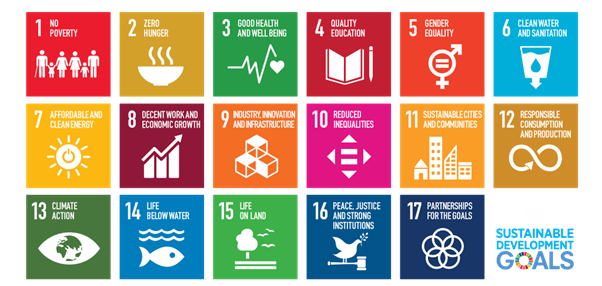
\includegraphics[width=0.8\textwidth]{Figures/Picture1}
    \caption{The seventeen United Nations Sustainable Development Goals \cite{un2015agenda}}
    \label{fig:sdg}
\end{figure}

The contribution of the project can be stated more precisely in terms of the targets that sit under each goal in the 2030 Agenda \cite{un2015agenda}. Under SDG 10, target 10.2 calls for the social, economic and political inclusion of all people irrespective of disability, and Silent Signals serves this target directly, because it lets a person with a hearing or speech impairment speak for themselves at a bank counter, a government office or a workplace instead of depending on a relative. Under SDG 4, target 4.5 calls for equal access to all levels of education for vulnerable people, including persons with disabilities, and the system supports it by giving a student a way to ask questions and take part in class discussion without an interpreter. Under SDG 3, target 3.8 calls for access to quality essential health-care services, and a patient who can describe symptoms to a doctor directly, in privacy, receives better care than one whose words are passed on by a family member. The contribution to these targets will be judged in FYP-II through user testing in realistic settings, by recording whether participants can complete everyday tasks such as asking for help, describing a problem and answering a question without assistance. Because the system runs on an ordinary phone or laptop and uses open source tools, it can reach the low-income families and public institutions in Pakistan for whom interpreters and specialised hardware are out of reach, which is where the inequality addressed by SDG 10 is greatest.

\section{Constraints}
The project is developed under several constraints that limit what can be delivered within two semesters. The first constraint is time, since the system contains several machine learning modules, a backend service and a user facing application, and all of them must be built, integrated and tested by a team of three students alongside other coursework. The second constraint is data. The lip-reading model is trained on the LRW dataset \cite{ref:Chung:2016}, which fixes the vocabulary to 500 broadcast English words, and public ASL datasets such as WLASL \cite{ref:Li:2020} contain isolated signs only, so the recognisers cannot be expected to cover free conversation in this phase. The third constraint is hardware. Model training is carried out on the team's own local GPU, whose memory limits the size of the models and the length of training runs, and the deployed system must run on a server and mid-range consumer devices with a phone camera or webcam, which rules out the largest published models. The fourth constraint is language, since the system supports English only and the ASL vocabulary is limited to common everyday signs. Finally, privacy and safety impose constraints on the design: video of users is processed and not stored, guardian contact details are held only for the purpose of notifications, and the emergency feature must keep working when non-critical modules such as the language model fail. These constraints are carried forward into the non-functional requirements of Chapter~\ref{ch:srs} and the general constraints of the design in Chapter~\ref{ch:design}.

\section{Business Opportunity}
Hearing loss affects a very large and growing population, which creates a steady need for tools that make communication easier \cite{who2021}. Institutions that serve the public, such as schools, hospitals, banks and offices, deal with customers who have hearing or speech impairments but rarely have trained interpreters available. Hiring an interpreter for every interaction is costly and often not possible, and specialised hardware such as speech generating devices is out of reach for many families. Silent Signals offers a lower cost option because it runs on a standard camera, on a laptop or phone, and uses open source tools. The main customers would be educational institutions, hospitals and clinics, banks and large employers, together with non-profit organisations and families who support people with impairments. Compared with audio based speech recognition, the system has a clear advantage because it works when the user cannot speak clearly and when the background is noisy.

Several routes to revenue are possible. A free basic version could serve individuals, while an institutional licence could be sold to a school or hospital for a yearly fee per site or per number of users. Premium features such as larger sign language vocabularies, additional languages and integration with hospital or school systems could be offered as paid add-ons. Partnerships with organisations that support people with disabilities could help to collect more training data and to reach users. The modular design also means that individual components, such as the lip-reading model or the noise suppression service, could later be offered to other developers through an interface. In the near term the project remains an academic prototype, and the opportunity described here is a possible direction for future work. Any such step would need validation with real users and a study of the market, which is outside the scope of this report.

\section{Stakeholders Description/ User Characteristics}
Silent Signals is used by several groups of people, and their needs shape many of the requirements in later chapters. The primary users are people with hearing or speech impairments who want to take part in conversations without the help of a relative or an interpreter. Some of them communicate by moving their lips without producing clear sound, and others communicate through sign language. The secondary users are the hearing people with whom they talk, such as teachers, doctors and bank staff, who read the recognized text or hear the spoken reply. Guardians and family members are also involved, since they are notified when the user needs help. The users are expected to have basic ability to operate a web interface, such as pressing buttons and reading text on a screen, and to have a device with a camera. They are not expected to have any knowledge of machine learning. Because the primary users may also have difficulty with small text or low contrast, the interface offers adjustable accessibility settings. The following subsections summarize the stakeholders and describe their goals and problems.

\subsection{Stakeholders Summary}
Table~\ref{tab:stake} summarizes the stakeholders of Silent Signals together with a short description and their role in the system. The stakeholders fall into four groups. Direct users give input to the system, namely the speech impaired user and the sign language user, who communicate through lip movements or signs. Receiving users are the hearing conversation partners and the guardians, who read the text, hear the speech or receive an alert. Adopting stakeholders are the institutions that choose to offer the system to their students, patients or customers, and they care mainly about cost and reliability. Finally, the development team and the supervisor build and evaluate the system. A single person can belong to more than one group, for example a student who signs in a classroom and later uses lip reading in a hospital. The roles in the table are the basis for the use cases that are described in Chapter~\ref{ch:srs}.
\begin{table}[!h]
\centering
\caption{Stakeholders of Silent Signals}
\begin{tabular}{|p{3.2cm}|p{5.8cm}|p{5cm}|}
\hline
\textbf{Stakeholder} & \textbf{Description} & \textbf{Role in the system} \\
\hline
Speech impaired user & A person who cannot produce clear speech but can move the lips & Uses lip-reading mode to communicate \\
\hline
Sign language user & A deaf or hard of hearing person who communicates through signs & Uses sign language mode to communicate \\
\hline
Hearing conversation partner & A teacher, doctor, bank officer or colleague who does not know sign language & Reads the text and hears the spoken reply \\
\hline
Guardian & A registered family member or caregiver of the user & Receives emergency notifications \\
\hline
Institution & A school, hospital, bank or workplace that serves such users & Adopts the system for its students, patients or customers \\
\hline
Development team and supervisor & The students who build the system and the project advisor & Design, build, test and evaluate the system \\
\hline
\end{tabular}
\label{tab:stake}
\end{table}

\subsection{Key High-Level Goals and Problems of Stakeholders}
Table~\ref{tab:goals} lists the key goals and problems of each stakeholder. The goals column states what the stakeholder wants to achieve, and the problems column states what currently prevents it. Many requirements of the system come directly from this table. For example, the problem of a guardian who cannot be present or reached in time leads to the emergency notification feature, and the problem of noise for the hearing conversation partner leads to the sound optimization module. Problems that are shared by several stakeholders, such as the scarcity of interpreters and the failure of audio based tools in noisy places, are the main motivation for the whole project. The table also shows that the needs of the groups are connected, because a system that serves the user well but is hard for the hearing partner to follow would not enable real conversation. The design therefore considers both sides of every conversation, and the requirements and use cases in later chapters are written with these goals and problems in mind.
\begin{table}[H]
\centering
\caption{Key goals and problems of the stakeholders}
\begin{tabular}{|p{3.2cm}|p{5.4cm}|p{5.4cm}|}
\hline
\textbf{Stakeholder} & \textbf{Key goals} & \textbf{Key problems} \\
\hline
Speech impaired user & Talk to hearing people and get help in an emergency & Interpreters are scarce and audio tools fail \\
\hline
Sign language user & Be understood by people who do not sign & Others do not understand signs \\
\hline
Hearing conversation partner & Understand the user quickly and reply naturally & Noise, unclear speech and no sign knowledge \\
\hline
Guardian & Know when the user needs help & Cannot be present or reached in time \\
\hline
Institution & Serve these users at low cost & Interpreters are costly and often unavailable \\
\hline
Development team and supervisor & Deliver an accurate working system on time & Limited data, hardware and time \\
\hline
\end{tabular}
\label{tab:goals}
\end{table}

\section{Conclusion}
This chapter has set out the vision of Silent Signals. The problem is the daily communication barrier faced by people with hearing or speech impairments in classrooms, hospitals, banks and workplaces, where interpreters are scarce, assistive hardware is costly and audio based speech recognition does not help a user who cannot speak clearly. The proposed solution is a single affordable platform that recognises speech from lip movements and signs, speaks the result aloud, and supports the user with confidence scores, language model correction, emotional context, conversation history and an emergency mode. The goals and objectives were stated so that each can be checked by demonstration, the scope was fixed to English and to a standard camera, and the deliverables and exclusions were listed. The work supports SDG 10, SDG 4 and SDG 3 through specific targets on inclusion, education and access to health care, and it is developed under constraints of time, data, hardware, language and privacy. The business opportunity lies with institutions that serve the public and cannot afford interpreters for every interaction, and the stakeholders range from the primary users and their conversation partners to guardians, institutions and the development team. The next chapter reviews the research on which each module of the system is built, so that the design choices in later chapters can be justified against the published state of the art.

\chapter{Literature Review / Related Work}
\label{ch:lit}
This chapter reviews the research on which Silent Signals is built. The system combines several problems that are normally studied separately, namely lip reading, sign language recognition and translation, speech recognition and synthesis, and the supporting tasks of text correction, noise suppression, facial expression recognition and landmark detection. Fifteen studies are reviewed, grouped into five categories that follow the modules of the system, so that every module described in the project proposal is supported by related work. For every study the review gives a summary of the method and its results, a critical analysis of its strengths and weaknesses, and the relationship of the study to our work. The lip-reading studies are reviewed first, because lip reading is the main module of the project, followed by sign language, the speech channel and the supporting modules. The chapter closes with a summary table of all fifteen studies and a conclusion that identifies the gap that Silent Signals addresses. All results quoted here are those reported by the authors of each study.

\section{Definitions, Acronyms, and Abbreviations}
The reviewed studies use a number of technical terms and acronyms that are not defined in Chapter~\ref{ch:vision}, and many of them appear in more than one review. They are collected here so that each term is explained once and the reviews can be read without reference to the original papers. Terms related to model architectures are listed first, followed by the loss functions and evaluation measures used to train and compare the models, and finally the terms specific to sign language and speech. The evaluation measures matter most when reading the summary table at the end of the chapter, because the studies report their results in different ways: translation work uses BLEU, recognition work uses word error rate or accuracy, and speech synthesis uses listening scores. These values can therefore be compared only within a category and not across categories. The list below gives each term with the meaning in which it is used in this chapter.
\begin{itemize}
  \item ASL: American Sign Language, used by the Deaf community in the United States and Canada.
  \item CNN: Convolutional Neural Network, a deep learning model that learns image filters.
  \item 3D CNN: a convolutional network whose filters span space and time, so it captures motion.
  \item RNN, GRU, LSTM: recurrent networks for sequences; GRU and LSTM are gated variants.
  \item HMM: Hidden Markov Model, a statistical model of sequences with hidden states.
  \item Attention: lets a model focus on the most relevant frames or words for each output word.
  \item Transformer: a network architecture based on multi-head attention instead of recurrence.
  \item Seq2Seq: an encoder-decoder model that maps one sequence to another sequence.
  \item CTC: Connectionist Temporal Classification, a loss that needs no frame-level alignment.
  \item Self-supervised learning: learning from unlabelled data by solving a task built from it.
  \item Gloss: a word-for-word written label for each sign in a signed sentence.
  \item SLR and SLT: Sign Language Recognition (video to glosses) and Translation (video to text).
  \item BLEU-4: a translation score based on overlapping phrases of up to four words.
  \item WER: Word Error Rate, the share of words substituted, inserted or deleted.
  \item ASR: Automatic Speech Recognition, also called speech-to-text.
  \item TTS: Text-to-Speech, the generation of spoken audio from text.
  \item Mel spectrogram: a time-frequency picture of audio on a scale close to human hearing.
  \item Vocoder: a model that turns a spectrogram back into an audio waveform.
  \item MOS: Mean Opinion Score, a listening test score from 1 to 5 for speech quality.
  \item N-best list: the top few candidate transcriptions produced by a recogniser.
  \item LLM: Large Language Model, a large transformer trained on general text.
\end{itemize}

\section{Detailed Literature Review}
\label{sec:lit-detailed}
This section reviews fifteen studies in five categories, presented in order. The first category, lip reading, covers Assael et al. \cite{assael2016lipnet}, Chung and Zisserman \cite{ref:Chung:2016} and Afouras et al. \cite{ref:Afouras:2018}, which form the basis of our main module. The second, sign language recognition, covers Koller et al. \cite{koller2016deepsign} and Li et al. \cite{ref:Li:2020}, which identify individual signs and define the model and data used by our sign module. The third, sign language translation, covers Camg\"oz et al. \cite{ref:Camgoz:2018}, Zhou et al. \cite{ref:ZhouB:2023} and Chen et al. \cite{ref:Chen:2026}, which turn signs into full sentences. The fourth, speech-to-text and text-to-speech, covers Baevski et al. \cite{baevski2020wav2vec}, Radford et al. \cite{radford2023whisper} and Shen et al. \cite{shen2018tacotron2}, which convert the hearing partner's speech into text and the recognised text into speech. The fifth, supporting modules, covers language model correction \cite{ma2023llmasr}, noise suppression \cite{valin2018hybrid}, facial expression recognition \cite{savchenko2022hsemotion} and landmark detection \cite{lugaresi2019mediapipe}. Each study is described with a summary, a critical analysis and its relationship to the proposed work.

\subsection{LipNet: End-to-End Sentence-level Lipreading}
\subsubsection{Summary of the research item}
Before LipNet, most lip-reading systems worked on single words or phonemes and relied on hand-designed visual features followed by a separate classifier. Assael et al. \cite{assael2016lipnet} proposed the first model that maps a variable-length sequence of mouth frames directly to a sentence, trained end to end with no intermediate labels. The network has three parts. Three layers of 3D convolutions look at short windows of frames so that the model captures lip motion rather than single images. Two bidirectional GRU layers then model the whole sequence in both directions. Finally, the CTC loss is used so that the model needs only the sentence and not a frame-level alignment between video and text. The model was trained and tested on the GRID corpus \cite{cooke2006grid}, in which 34 speakers read short fixed-grammar sentences under controlled lighting. The mouth region was cropped with a landmark detector, and data augmentation such as horizontal mirroring was used. The model predicts characters, which are joined into words by a beam search decoder.

\subsubsection{Critical analysis of the research item}
The main strength of this work is that it showed sentence-level lip reading is possible with a single network. On GRID it reached a word error rate of about 4.8\% on speakers seen during training and about 11.4\% on unseen speakers, far better than experienced human lip readers on the same data. The use of CTC removed the need for expensive alignment, and the 3D convolutions showed that modelling motion across frames matters more than looking at single frames. The weakness is the dataset. GRID sentences follow a fixed six-word grammar with a vocabulary of only 51 words, the camera is frontal and the lighting is fixed, so the high accuracy says little about performance in a classroom or hospital with an ordinary webcam. The model never encountered pose changes, motion blur or different frame rates. Because the output is character based, the decoder can also produce non-words when the visual input is ambiguous, which is why later systems add a language model.

\subsubsection{Relationship to the proposed research work}
LipNet is the direct ancestor of the lip-reading module in Silent Signals. Our pipeline follows the same overall design: landmark-based mouth cropping, a 3D convolutional front end to capture motion, a recurrent back end, and training on sequences of mouth frames rather than single images. Its results also justify two of our design decisions. First, since the model is weakest on unseen speakers, we evaluate our model on speakers that are not in the training set, as described in Chapter~\ref{ch:approach}. Second, since ambiguous lip movements lead to wrong or invalid words, we add a language model correction step after the lip-reading model and show a confidence score for each word, so that the user can see where the model was unsure. The limitations of GRID are the reason we train on the more natural LRW dataset reviewed next, since a model that only works on frontal studio video would not help a user in a hospital or a bank.

\subsection{Lip Reading in the Wild}
\subsubsection{Summary of the research item}
Chung and Zisserman \cite{ref:Chung:2016} set out to recognise the words spoken by a talking face using only video, and addressed the main problem with earlier lip-reading datasets, which were small, recorded in laboratories and limited to a few speakers. Their paper makes two contributions. The first is a pipeline that collects data automatically from BBC television by aligning subtitles with the audio, detecting and tracking faces, and cutting out short clips in which a target word is spoken. The result is the Lip Reading in the Wild (LRW) dataset, with up to 1000 utterances for each of 500 words, spoken by over a thousand different people with natural variation in pose, lighting and accent. The second contribution is a set of VGG-based CNN architectures that classify which of the 500 words was spoken from the mouth frames alone. The authors compare networks that process frames separately with networks that combine frames, so the study also compares ways of handling the time dimension.

\subsubsection{Critical analysis of the research item}
The strongest point of the work is the dataset. Earlier lip-reading datasets were limited in both the number of speakers and the size of the vocabulary, which made it hard to evaluate models on a diverse range of faces. Manual labelling at this scale would be too expensive, and the automatic pipeline avoids it by using subtitles as weak labels, an idea since reused in sign language work. LRW became the standard benchmark for word-level lip reading, and the best network in the paper reached about 61\% top-1 accuracy over 500 words. Later work combining 3D convolutions with residual networks and recurrent layers raised the accuracy considerably, showing that the dataset could support deeper models. The main weakness is that the task is classifying isolated words from a closed set of 500, not reading sentences. Each clip contains one target word near its centre, so the model never has to find where words begin and end, and the clips come mostly from clear, well-lit and frontal television speakers.

\subsubsection{Relationship to the proposed research work}
LRW is the dataset on which the lip-reading module of Silent Signals is trained and evaluated, so this paper describes the data our model learns from. Its speaker variety is what we need for a system that will be used by people who were never in the training set. The paper also makes the limits of our approach clear: a model trained on LRW recognises words from a fixed vocabulary, which is why the system shows a confidence score for each word, lets the user correct uncertain words, and treats the vocabulary as something to extend in later work. The pre-processing in Chapter~\ref{ch:approach}, which crops a fixed-size mouth region from each frame using facial landmarks, follows the face tracking and cropping stage of this pipeline. The comparison of designs in this paper, together with the later gains from 3D convolutions and recurrent layers, is the reason our model combines a 3D CNN with a bidirectional LSTM.

\subsection{Deep Audio-Visual Speech Recognition}
\subsubsection{Summary of the research item}
Afouras et al. \cite{ref:Afouras:2018} address the recognition of phrases and sentences spoken by a talking face, with or without audio. Rather than limiting the task to a few words, they treat lip reading as an open-world problem of unconstrained sentences in videos recorded in the wild. They make three main contributions. First, they compare two transformer-based lip-reading models, one trained with a CTC loss and the other with a sequence-to-sequence loss, both using a visual front end of 3D convolutions and a residual network. Second, they study how much lip reading helps audio speech recognition in noise, using a model trained on both audio and video and deliberately corrupting the audio with babble noise at several levels. Third, they release LRS2-BBC, a dataset of thousands of natural sentences from British television, and the journal version adds LRS3-TED, built from TED and TEDx talks. An external language model is used during decoding to improve the output.

\subsubsection{Critical analysis of the research item}
A strong point of this paper is that it moves lip reading from isolated words to full sentences. The authors report that their models outperform all previous lip-reading models by a large margin, and the comparison of CTC and sequence-to-sequence models gives practical insight into the trade-off between them. The noise study is also important: the audio-visual model performed better than audio alone, and the gap grew as the noise increased, showing that the lips carry information that complements the sound. The weaknesses are practical. The lips-only model still had a word error rate of around 50\% on LRS2, so vision alone is far from reliable on open speech, partly because some sounds look identical on the mouth. The models are large, were trained on hundreds of hours of video with substantial GPU resources, and are not designed for real-time use on an ordinary laptop. The data also consists mostly of well-lit frontal faces from television.

\subsubsection{Relationship to the proposed research work}
This study sets realistic expectations for Silent Signals. Our users may not be able to produce audio at all, so the lips-only results are the ones that matter, and they tell us that a lip-reading model will make many mistakes on open speech. This is why the project limits the lip-reading vocabulary, shows a confidence score for each word and passes the output through a language model before it is spoken, which mirrors the external language model used in this paper's decoder. The finding that the visual stream helps most when audio is noisy also supports noise suppression on the hearing partner's side of the conversation, since the two channels fail in different conditions. The idea of combining two input streams and measuring the contribution of each is also useful for our design, in which lip reading and sign recognition share one interface. Finally, the 3D convolution and residual network front end belongs to the same family of designs as our module.

\subsection{Deep Sign: Hybrid CNN-HMM for Continuous Sign Language Recognition}
\subsubsection{Summary of the research item}
Koller et al. \cite{koller2016deepsign} addressed continuous sign language recognition, where a model must recognise a sequence of signs without being told where one sign ends and the next begins. Before this work, most systems used hand-crafted features with statistical sequence models, and deep networks had mainly been applied to isolated signs. The authors embedded a convolutional neural network inside a hidden Markov model, so that the network estimates the probability of each hidden state from a frame and the HMM handles the timing and order of the signs. Because frame-level labels do not exist, they used an iterative scheme: an existing system provides an initial alignment of frames to states, the network is trained on it, the improved network re-aligns the data, and the process repeats. The network input is a crop of the dominant hand in each frame. The system was evaluated on RWTH-PHOENIX-Weather 2014 \cite{koller2015phoenix} and SIGNUM \cite{vonagris2008signum}, where it clearly reduced the word error rate of earlier statistical systems.

\subsubsection{Critical analysis of the research item}
The main strength of this work is that it showed how a deep network could be used for continuous recognition when only sentence-level labels are available, by letting a sequence model handle alignment and repeatedly refining the training targets. This idea of solving alignment and recognition together reappears in the later CTC-based models. The use of hand crops also shows that much of the information in signing is carried by the shape and movement of the dominant hand, which is a useful guide to the choice of input. The weaknesses are also clear. Looking only at the dominant hand ignores the other hand, the face and the body, which carry grammatical information such as questions and negation. The iterative alignment depends on a good initial system and is slow to train. The error rates, although improved, remained too high for the output to be used directly for communication, and the data again consisted of German weather forecasts performed by a small number of signers.

\subsubsection{Relationship to the proposed research work}
This study explains two decisions in our sign language module. First, it shows the value of cropping the relevant region before passing it to a network, which our pipeline does when it uses hand and body landmarks to locate the signer before recognition. Second, its limitation of looking at only one hand is why our module keeps the upper body and both hands in its input, since many everyday signs use both hands and depend on where the hands are relative to the body. The high error rates of continuous recognition reported here also support our decision to recognise signs from a limited vocabulary and to let the user confirm the result, rather than attempting continuous recognition of unconstrained signing in this phase. Finally, HMM-based alignment has since been largely replaced by CTC and transformer models, so we use this paper as background on how the field reached its current methods rather than as a design to copy.

\subsection{Word-level Deep Sign Language Recognition from Video}
\subsubsection{Summary of the research item}
Li et al. \cite{ref:Li:2020} noticed that most sign language datasets contained only a small number of words, so models trained on them could not be used in real situations. To address this, they introduced WLASL, a Word-Level American Sign Language video dataset with more than 2000 words performed by over 100 signers, collected from online educational sources and checked manually. They describe it as by far the largest public ASL dataset for word-level recognition. The paper also implements and compares two families of baseline methods. The first uses the visual appearance of the video, with a 2D CNN followed by a recurrent network and with an Inflated 3D ConvNet (I3D) pretrained on action recognition. The second uses 2D human pose, where body and hand keypoints extracted from each frame are fed to a recurrent network, and a pose-based temporal graph convolution model is proposed to improve on it. The dataset is released in subsets of 100, 300, 1000 and 2000 words.

\subsubsection{Critical analysis of the research item}
The main strength is that the dataset fills a clear gap, and the baselines give other researchers something to compare against. It is also interesting that the pose-based and appearance-based models perform at similar levels, with the best reaching approximately 66\% top-10 accuracy on the 2000-word subset, which shows that both approaches work but that the task remains challenging. The clear drop in accuracy as the vocabulary grows from 100 to 2000 words is a useful warning for anyone designing a recogniser. The main drawback is that each sample is a single word. The dataset contains no sentences, so there is no grammar and no information about how signs combine, and it cannot be used to train a complete translation system on its own. Because the videos come from many online sources, recording conditions and signing speed vary, and some classes have very few examples, which makes the rarer words in the vocabulary hard to learn.

\subsubsection{Relationship to the proposed research work}
WLASL is the most directly useful dataset for our project, because the sign language module of Silent Signals recognises ASL signs from a vocabulary of everyday words, which is exactly the task this paper defines. The I3D baseline reported here is the model family that our module builds on, and the accuracy on the smaller subsets gives a realistic target for a vocabulary of the size we plan to support. The paper also shows how recognition becomes harder as the number of words increases, which is why we limit the vocabulary in FYP-I and extend it gradually. Its finding that pose information is a serious alternative to raw video matters because our landmark detector already produces hand and body keypoints, and a pose-based model would be lighter to run. The lack of sentence structure in WLASL is the reason our module produces a sequence of words that is then passed to the language model correction step rather than a finished sentence.

\subsection{Neural Sign Language Translation}
\subsubsection{Summary of the research item}
Traditionally, sign language recognition systems mapped one sign to one word rather than producing a full sentence. Camg\"oz et al. \cite{ref:Camgoz:2018} formalised Sign Language Translation (SLT) as a Seq2Seq problem, shifting the objective from isolated sign prediction to generating natural spoken language sentences directly from video. Their end-to-end framework pairs a 2D CNN, which extracts spatial features from each frame, with a GRU-based encoder-decoder, and an attention mechanism, tested in Bahdanau \cite{bahdanau2015attention} and Luong \cite{luong2015attention} variants, lets the decoder focus on different parts of the video while producing each word. Two setups were compared: an end-to-end model that translates directly from frames, and a hybrid model that first recognises intermediate gloss annotations and then translates the glosses into text. The authors also introduced the RWTH-PHOENIX-Weather 2014T (PHOENIX14T) dataset \cite{ref:Camgoz:2018} of 8,257 German Sign Language weather-forecast videos, each paired with glosses and a German translation. It was the first public dataset of this kind and became the common benchmark of the field.

\subsubsection{Critical analysis of the research item}
One strength of this work is that it showed SLT could be learned end to end without glosses at inference time, which makes the approach easier to extend to new data. The experiments also showed that attention clearly improves translation over a plain encoder-decoder, and the gloss-to-text result of 19.26 BLEU-4 gave a useful upper bound for end-to-end models. Releasing PHOENIX14T was arguably just as important, since later work has relied on it heavily. However, the study has several limitations. The end-to-end model reached only about 9.6 BLEU-4, around half of the gloss-based upper bound, so direct video-to-text translation was still far from usable. The dataset covers one small domain, weather forecasts, with a small vocabulary and few signers, so the results may not carry over to everyday conversation. The visual features come from a frame-level 2D CNN pretrained on ImageNet rather than on sign data, so motion between frames is not modelled directly, and the recurrent decoder struggles with long sentences.

\subsubsection{Relationship to the proposed research work}
This research is directly relevant to our project, whose sign language module converts ASL into English text. Camg\"oz et al. \cite{ref:Camgoz:2018} showed that sign language can be treated as translation over full sentences rather than word-by-word recognition, and this idea sets the long-term direction of our module. Their results also explain why we do not start there. A BLEU-4 score below ten on a narrow weather domain shows that sentence-level translation from video was not yet reliable enough for a product, and it required gloss-annotated data that does not exist at a comparable scale for ASL. Silent Signals therefore begins by recognising signs from a vocabulary of everyday words and passes the recognised words to a language model that forms the sentence. The finding that attention helps the model focus on the relevant frames also supports our use of a temporal model rather than single-frame classification. Finally, their focus on German Sign Language leaves room for work on ASL to English, the language pair our users need.

\subsection{Gloss-Free Sign Language Translation via Visual-Language Pretraining}
\subsubsection{Summary of the research item}
Zhou et al. \cite{ref:ZhouB:2023} argue that glosses are both an information bottleneck and an expensive annotation requirement, and that sign language translation should not depend on them. Their method, GFSLT-VLP, initialises the visual and text components from pretrained vision-language models so that the system inherits semantic knowledge before seeing any sign language data. In a first stage, the visual encoder is trained to align video features with the text of the matching sentence using a contrastive objective, in the same way that image-text models are trained. In a second stage, the whole model is fine-tuned end to end on sign-to-text pairs without any gloss supervision. On PHOENIX14T \cite{ref:Camgoz:2018} the method improves over previous gloss-free methods by more than 5 BLEU-4, and on CSL-Daily \cite{zhou2021csldaily} by more than 3 BLEU-4 \cite{ref:ZhouB:2023}, while being competitive with several gloss-based approaches. An analysis of the components shows that the alignment stage is the main source of the improvement.

\subsubsection{Critical analysis of the research item}
The main takeaway is not simply that the BLEU score increased, but that an approach without glosses closed most of the gap to approaches that use gloss supervision. Glosses are therefore shown to be unnecessary, and models can be trained on video that has never been annotated for glosses, which is the great majority of sign language data. Visual-language pretraining is a logical answer to the small size of sign language datasets, since it borrows knowledge from large general-purpose corpora. At the same time, the evaluation is limited to restricted domains. PHOENIX14T \cite{ref:Camgoz:2018} covers only weather with a very limited vocabulary, so good results there do not guarantee good results in open conversation. Moreover, the visual aspects of signing, in particular hand shapes, spatial grammar and facial markers, may not transfer from general pretraining as well as the objects and scenes those models were trained on. The model is also large, which limits its use on ordinary hardware.

\subsubsection{Relationship to the proposed research work}
This is probably the most directly applicable methodological paper for the long-term direction of our sign language module. As with any sign language system, our ASL data is limited, and producing gloss annotations would be a major bottleneck for a team of three students. The gloss-free approach shows that a future sentence-level version of Silent Signals could be trained on datasets such as How2Sign \cite{duarte2021how2sign} or YouTube-ASL \cite{ref:Uthus:2023} that have video and English text but no gloss labels, by starting from a strong pretrained model and fine-tuning it on ASL-to-English pairs. For the present project the lesson is more modest but still useful. Our sign recogniser starts from a pretrained video model rather than from random weights, for the same reason that this paper starts from pretrained vision-language models, namely that sign language data is too scarce to learn visual features from scratch. The paper's warning that sign-specific cues may not transfer is also why we evaluate the recogniser on signers absent from the training data.

\subsection{Improving Sign Language-Gloss Translations With Pretrained Models}
\subsubsection{Summary of the research item}
In traditional SLT systems, sign language video is first converted into glosses by continuous recognition, and a neural machine translation model then translates the glosses into spoken language text. Annotated sign language data for training such translation models is scarce, and there was a long-standing assumption that converting glosses to text is like translating between two different languages, such as English and German. Chen et al. \cite{ref:Chen:2026} showed this assumption to be untrue: glosses and the target sentence share most of their vocabulary and differ mainly in word order, function words and inflection. They therefore framed gloss-to-text as a monolingual constrained generation, or denoising, task. They found that models pretrained to repair corrupted text through denoising auto-encoding, such as mBART, performed much better than models trained for conventional translation. The idea was evaluated on three benchmarks, PHOENIX14T \cite{ref:Camgoz:2018}, ASLG-PC12 \cite{othman2012aslgpc12} and CSL-Daily \cite{zhou2021csldaily}, against standard transformer baselines trained from scratch on the same data.

\subsubsection{Critical analysis of the research item}
This work presents a clear approach to the low-resource nature of gloss-to-text translation and disproves an old assumption. Another major strength is that the approach is evaluated on three benchmarks in different sign languages and improves translation quality on all of them, which suggests that the finding is general rather than specific to one language pair. Using a large pretrained text model is also attractive for small datasets, because most of the linguistic knowledge comes from general text rather than from the few thousand sign language sentences available. However, the approach has limitations. The primary one is that it focuses on gloss-to-text translation rather than direct video-to-text translation, so it does not address the difficult recognition stage. It may also be sensitive to noisy or incorrectly recognised glosses, which could reduce its effectiveness when the glosses come from a real recogniser. Furthermore, the evaluation relies on automatic measures such as BLEU, ROUGE and METEOR, which may not fully reflect quality as judged by human readers.

\subsubsection{Relationship to the proposed research work}
This study is relevant to Silent Signals because it shows how effective pretrained sequence-to-sequence models are at turning a sequence of sign labels into fluent text. Our sign language module produces a sequence of recognised words, which is close to a gloss sequence, while the hearing partner needs a natural English sentence. The finding that this step is monolingual denoising rather than translation supports the design of our context based correction module, which uses a pretrained language model to repair raw recogniser output instead of a translation model trained from scratch. Sign language translation in Silent Signals is therefore performed in two steps, recognition of individual signs followed by sentence formation with a pretrained language model. It also supports using one correction module for both the lip-reading and the sign language outputs, since in both cases the task is to turn a noisy English word sequence into a correct sentence. The sensitivity of the approach to recognition errors is why we show a confidence score for each recognised word and let the user confirm the corrected sentence before it is spoken, and its reliance on automatic measures reminds us to include human judgement in our own evaluation.

\subsection{wav2vec 2.0: A Framework for Self-Supervised Learning of Speech Representations}
\subsubsection{Summary of the research item}
Speech recognition models traditionally need thousands of hours of transcribed audio, which is expensive to produce and unavailable for most languages and settings. Baevski et al. \cite{baevski2020wav2vec} proposed wav2vec 2.0, a framework that first learns speech representations from unlabelled audio and then needs only a small amount of transcribed speech to become an accurate recogniser. A convolutional encoder turns the raw waveform into a sequence of latent features, parts of this sequence are masked, and a transformer must identify the correct quantised version of each masked feature among a set of distractors, which is a contrastive self-supervised task. After pre-training on tens of thousands of hours of unlabelled audiobook speech, the model is fine-tuned for transcription with a CTC loss on labelled data. On the LibriSpeech benchmark \cite{panayotov2015librispeech}, fine-tuning on only ten minutes of transcribed speech gave word error rates of about 4.8\% and 8.2\% on the clean and noisy test sets, and fine-tuning on all 960 hours gave 1.8\% and 3.3\%.

\subsubsection{Critical analysis of the research item}
The main strength of this work is that it showed speech recognition can be learned mostly from unlabelled audio, which changed what is possible for settings with little transcribed data. The results with ten minutes or one hour of labels were remarkable at the time, and the same pre-trained model can be fine-tuned for many tasks and languages, which is why it became a standard starting point. Learning directly from the waveform also removes the need for hand-designed audio features. The weaknesses are mostly practical. Pre-training is extremely expensive and needs large GPU clusters, so in practice only released checkpoints can be used. The best low-resource results also relied on an external language model during decoding. The data is read English audiobooks, which are cleaner than conversation in a busy hospital or bank, so performance on spontaneous and noisy speech is lower. Finally, the model still needs a fine-tuning step for each new task, unlike later models that work out of the box.

\subsubsection{Relationship to the proposed research work}
The speech-to-text module of Silent Signals converts the hearing partner's spoken reply into text, so that a user with a hearing impairment can read what was said and the two-way conversation can continue. wav2vec 2.0 is relevant because it shows that an accurate recogniser can be built from a pretrained model with very little labelled data, which matters if the module later has to be adapted to the accents and vocabulary of Pakistani speakers, for whom little transcribed English speech is available. It also explains the role of the language model in our design: its best results came from combining the acoustic model with a language model, which supports passing all recognised text through our correction module. However, the need for fine-tuning and the drop in accuracy on noisy, spontaneous speech mean that wav2vec 2.0 is not the most practical choice for our first version. These limitations lead directly to the model reviewed next, which is designed to work robustly without fine-tuning.

\subsection{Robust Speech Recognition via Large-Scale Weak Supervision}
\subsubsection{Summary of the research item}
Radford et al. \cite{radford2023whisper} asked whether a speech recogniser trained on a very large and varied set of imperfectly transcribed audio could work well on new data without any fine-tuning. They collected about 680,000 hours of audio paired with transcripts from the internet, covering many languages, speakers, accents and recording conditions, and trained an encoder-decoder transformer, called Whisper, that reads a log-Mel spectrogram of 30-second audio windows and writes the transcript. The same model is trained on several tasks at once, namely transcription, translation into English, language identification and the detection of speech, with special tokens telling the decoder which task to perform. Models of several sizes were released, from a small model with tens of millions of parameters to a large one with over a billion. Whisper was evaluated in a zero-shot setting on many existing benchmarks, and the authors report that it makes far fewer errors than models fine-tuned on LibriSpeech when both are tested on other datasets, approaching human robustness.

\subsubsection{Critical analysis of the research item}
The clearest strength of Whisper is robustness. Because it was trained on varied real-world audio, it handles accents, background noise and different recording equipment much better than models trained on a single clean dataset, and it does so without fine-tuning, which makes it practical to use directly. The release of the models as open source, in several sizes, also lets developers trade accuracy for speed according to their hardware. The weaknesses are known from the paper and later use. The model processes audio in 30-second windows rather than as a stream, so a short delay is unavoidable in live use. On silence or unclear audio it can produce text that was never spoken, repeating phrases or inventing words, which is risky in an assistive setting. The larger models need a GPU to run quickly, and accuracy is lower for languages and accents that are rare in the training data. Finally, the internet training data is not published, so its biases cannot be examined.

\subsubsection{Relationship to the proposed research work}
Whisper is the most suitable model for the speech-to-text module of Silent Signals. Our users meet hearing people in classrooms, hospitals and banks, where speech is spontaneous, accented and surrounded by noise, which is exactly the setting in which Whisper outperforms models trained on clean data. It also runs locally from open source models, so the hearing partner's speech does not have to be sent to an external service, which supports the privacy-centred design of the system, and a smaller model can be chosen to keep the delay acceptable on our server. Its limitations shape how we use it. Because it can invent text on silence or unclear audio, the partner's audio is first cleaned by the sound optimization module and checked for speech, and the transcript is shown to the user as text rather than acted on automatically. Its 30-second window design also means we transcribe each reply after the partner stops speaking rather than word by word.

\subsection{Natural TTS Synthesis by Conditioning WaveNet on Mel Spectrogram Predictions}
\subsubsection{Summary of the research item}
Shen et al. \cite{shen2018tacotron2} describe Tacotron 2, a neural text-to-speech system that produces speech from raw text in two stages. The first stage is a sequence-to-sequence network with attention that converts a sequence of characters into a mel spectrogram, a compact time-frequency representation of speech on the perceptual mel scale \cite{stevens1937mel}. The second stage is a modified WaveNet vocoder \cite{vandenoord2016wavenet} that turns the mel spectrogram into an audio waveform one sample at a time. Separating the stages means that the vocoder can be trained on spectrograms predicted by the first network, so the two parts fit together well, and the mel spectrogram is a far simpler target than the linguistic and acoustic features used by older concatenative or parametric systems. The system was trained on about 24 hours of speech from a single professional speaker. In a listening test the generated speech received a mean opinion score of about 4.5 out of 5, very close to the score given to real recordings of the same speaker, and listeners showed only a small preference for the real recordings.

\subsubsection{Critical analysis of the research item}
The strength of the work is quality. It showed that a fully learned pipeline can produce speech that listeners find almost indistinguishable from a human recording, and its two-stage design of an acoustic model followed by a neural vocoder has been the standard architecture of most text-to-speech systems since. Using the mel spectrogram as the interface between the stages is simple and has been reused widely. The weaknesses are speed and robustness. The WaveNet vocoder generates audio one sample at a time, which makes it slow for real-time use, and later systems replaced it with much faster vocoders. The attention mechanism can fail on long or unusual inputs by repeating or skipping words, and the model is tied to one speaker and one language, so a new voice needs many hours of new recordings. Rare words and names are sometimes mispronounced because the model works from characters, and the evaluation covers only read sentences rather than conversational speech.

\subsubsection{Relationship to the proposed research work}
The text-to-speech module of Silent Signals reads the recognised and confirmed sentence aloud, so that a hearing person can hear what the user said and reply naturally. Tacotron 2 \cite{shen2018tacotron2} defines what good neural speech synthesis looks like and the structure that modern speech engines follow. Because our system must respond with little delay on ordinary hardware, we do not train such a model ourselves but use an existing speech engine, which keeps the module simple and lets the team concentrate on lip reading and sign language. The weaknesses of the paper still shape our design. The input to our speech engine comes from a lip-reading or sign recognition model and may contain unusual words, so the sentence is first corrected by the language model and confirmed by the user before it is spoken, which reduces failures on malformed text. The requirement in Chapter~\ref{ch:srs} that speech begins within one second of confirmation follows from the slow vocoder problem described here, and rules out sample-by-sample synthesis.

\subsection{Can Generative Large Language Models Perform ASR Error Correction?}
\subsubsection{Summary of the research item}
Ma et al. \cite{ma2023llmasr} studied whether a general-purpose large language model can correct the mistakes of a speech recognition system without being trained for that purpose. Traditional error correction models are trained on the outputs of one specific recogniser, which is expensive and ties the corrector to that system. Instead, the authors prompted ChatGPT with the recogniser's N-best list, that is, the top few candidate transcriptions, and asked it to produce the correct sentence. Two variants were tested: an unconstrained version, in which the model may write any sentence, and a constrained version, in which it must choose one of the candidates. Both were run in zero-shot and one-shot settings, meaning that the model saw at most one example of the task. Experiments covered two modern recogniser types, a transducer and an attention-based encoder-decoder, on several standard test sets, and the change in word error rate after correction was measured. Examples of successful and failed corrections were also examined.

\subsubsection{Critical analysis of the research item}
The main finding is that a large language model with no task-specific training can reduce the word error rate of strong recognisers, and that giving it several candidates helps, because the alternatives show where the recogniser was unsure. This is a strength because correction can be added to a pipeline without collecting paired error data, which is expensive for any new recogniser. The constrained variant is also useful, since it cannot invent words that were never recognised, which makes its behaviour more predictable and safer. The weaknesses are that the gains are modest, that the unconstrained model sometimes rewrites correct sentences or adds content, and that the evaluation uses audio-based recognition, whose errors differ from those of a lip reader. The study also used a closed commercial model, so the results may not transfer to small open models that run locally, and latency and cost were not considered, although both matter for a real-time assistive application in which a reply is expected within seconds.

\subsubsection{Relationship to the proposed research work}
The context based correction module of Silent Signals does what this paper describes, but for visual speech and signs. A lip-reading model confuses sounds that look alike on the lips, such as those written with p, b and m, so a sentence such as ``I ant watr'' needs a language model to become ``I want water''. This work shows that a prompted language model can perform such correction with no extra training, which is the approach we take with a locally hosted Llama 3.2 model \cite{ollama_llama32_3b}. Its results guide two decisions. We supply the model with context, namely the recognised words with their confidence scores, the conversation history and the user's profile, in the same way that the N-best list supplies alternatives in this study. We also let the user disable correction and confirm each sentence, because the paper shows that an unconstrained model can change the meaning of a correct sentence. The same correction can also be applied to the transcripts produced by our speech-to-text module, which are recogniser output of exactly the kind studied in this paper. Using a small local model is our answer to the latency, cost and privacy concerns the paper leaves open.

\subsection{A Hybrid DSP/Deep Learning Approach to Real-Time Full-Band Speech Enhancement}
\subsubsection{Summary of the research item}
Valin \cite{valin2018hybrid} proposed RNNoise, a noise suppression method that combines classical signal processing with a small recurrent neural network so that it runs in real time on an ordinary CPU. Instead of asking the network to produce the clean waveform directly, the audio is divided into 22 frequency bands on a perceptual scale, and the network predicts only a gain for each band, which is then applied to the noisy spectrum. The network also outputs a voice activity decision, and a pitch filter removes noise between the harmonics of the voice, which the coarse band gains cannot reach. The network uses GRU layers and has about 215 thousand weights, several orders of magnitude fewer than typical enhancement networks. It was trained on clean speech mixed with many types of recorded noise at different levels, and it processes 48\,kHz full-band audio in 10\,ms frames, so it adds very little delay. The method is evaluated against a conventional spectral estimator and released as open source software.

\subsubsection{Critical analysis of the research item}
The strength of the work is its efficiency. Because the network predicts only a small number of band gains, it needs a tiny fraction of the computation of a full spectrogram-to-spectrogram network, which makes it usable on laptops and phones without a GPU, and it has been adopted in open source conferencing software. Combining learned gains with a hand-designed pitch filter is a sensible way to obtain both robustness and low cost, since the network handles what is hard to model by hand and the filter handles what is well understood. The paper shows better quality than the conventional baseline, especially for changing noise such as background chatter, which is typical of waiting rooms and banks. The limitations are that the evaluation relies mainly on objective measures and a small listening test, that one small model may not generalise to every noise type, and that heavy noise or several overlapping speakers can cause the network to suppress the speech it should keep.

\subsubsection{Relationship to the proposed research work}
The sound optimization module of Silent Signals performs the same task as RNNoise: keeping the hearing partner's spoken reply intelligible in a noisy classroom, hospital or bank. The approach is directly applicable because our system must run on ordinary hardware alongside the lip-reading model, so a lightweight hybrid design is preferable to a large enhancement network. The voice activity output also has a second use in our system, since it can tell the application when the hearing partner has finished speaking, so that the user can begin the next sentence. The paper's evaluation setup, with clean speech mixed with recorded noise at several levels, is the one we plan to follow when testing the module. Cleaning the partner's audio before it reaches the speech-to-text model also reduces transcription errors and the risk of invented text on noise. Its limitation with overlapping speakers is also a known limitation of our system, which is designed for a conversation between two people rather than a group. Because the implementation is small and open source, it could even run on the user's device, which supports the privacy goal of the project.

\subsection{HSEmotion: High-Speed Emotion Recognition Library}
\subsubsection{Summary of the research item}
Savchenko \cite{savchenko2022hsemotion} presents HSEmotion, an open source library of lightweight models for recognising facial expressions from a single face image in real time. The models are based on efficient convolutional networks such as MobileNet and EfficientNet. They are first trained on a large face identification dataset, so that they learn general facial features, and then fine-tuned on AffectNet \cite{mollahosseini2019affectnet}, a large collection of internet face images labelled with eight expressions, including happy, sad, angry and neutral, together with valence and arousal values. The library exposes a simple interface that takes a cropped face and returns the expression scores and a feature vector, and it is designed to run on a CPU or a mobile device at video frame rates. The author reports that the models reach accuracy close to the best published results on AffectNet \cite{mollahosseini2019affectnet} while being many times faster than the large networks behind those results. The feature vectors can also be averaged over the frames of a video to recognise the emotion of a whole clip.

\subsubsection{Critical analysis of the research item}
The strength of this work is that it makes expression recognition practical. Research models for AffectNet are often large ensembles that cannot run in real time beside other models, while HSEmotion offers networks small enough to run on every frame on ordinary hardware with only a small loss in accuracy, reported at over 60\% on the eight-class task. Pre-training on face identification is a useful idea, because facial features learned for identity transfer well to expressions. The weaknesses are those of the task itself. The AffectNet labels are noisy, and human annotators often disagree on the expression in an image, so accuracy near 60\% is close to the ceiling of the data. The models work on single frames, so their output can flicker between classes unless it is smoothed, and the training images are mostly photographs from the web, which may not resemble a person mouthing words in front of a webcam. As a software description, the paper's own evaluation is also brief.

\subsubsection{Relationship to the proposed research work}
Silent Signals detects four expressions, namely happy, sad, angry and neutral, to give the hearing partner some of the emotional context that tone of voice would normally carry, and this module must run at the same time as lip reading. A lightweight library of the HSEmotion type is therefore the right fit, and the four classes we need are a subset of its eight, so the model can be used directly with its output restricted to those classes. The limitations of the library shape our design. We smooth the predictions over several frames to remove flicker, and we show the expression as supporting information beside the text rather than as part of the recognised sentence. The face crop produced by our landmark detector can be passed directly to the model, so no extra face detector is needed. Because a user who is mouthing words moves the lower face constantly, which may confuse a model trained on still photographs, our evaluation will compare its output during speech and at rest.

\subsection{MediaPipe: A Framework for Building Perception Pipelines}
\subsubsection{Summary of the research item}
Lugaresi et al. \cite{lugaresi2019mediapipe} describe MediaPipe, an open source framework from Google for building real-time perception pipelines such as face, hand and body landmark detection. A pipeline is defined as a graph of components called calculators, where each node performs one step, such as decoding a frame, running a neural network or drawing results, and data flows between nodes as time-stamped packets. The framework handles the synchronisation of streams with different rates, scheduling across threads, and running the same graph on desktop, mobile and web platforms. The paper presents example graphs for object detection and face landmark tracking, and shows how an expensive detector can be combined with a cheap tracker so that the full detector runs only when tracking is lost. The ready-made solutions built on the framework provide dense face meshes, hand landmarks and body pose from a standard camera, and are available from Python through the MediaPipe Tasks interface \cite{googlemediapipe2026}, which is the interface our pipeline uses.

\subsubsection{Critical analysis of the research item}
The strength of MediaPipe lies in engineering rather than in a new model. It solves the practical problems of running several models on live video at the same time, with low delay and without a GPU, and its landmark models are accurate enough for most cropping and tracking tasks. Because the same graph runs on a laptop, a phone and a browser, it suits applications that must be cheap to deploy, and the detector-plus-tracker design is a simple and effective way to save computation. The weaknesses are that the landmark models are trained by Google on data that is not published, so their accuracy cannot be examined or improved by users, that performance drops when the face or hands are partly out of view or heavily turned, and that the framework is designed for running models rather than training them. The paper itself is a system description with few quantitative results, so the accuracy of the individual models has to be taken from separate reports.

\subsubsection{Relationship to the proposed research work}
MediaPipe is the backbone of the input side of Silent Signals. The face landmarker locates the lips in every frame so that a stable mouth region can be cropped for the lip-reading model, the hand and pose landmarkers locate the signer for the sign language module, and the face region found by the same detector is passed to the expression model. The design of the framework matches the real-time requirement of the project, because landmark detection, lip reading and expression recognition can all run as stages of one pipeline on an ordinary laptop. Its limitations also inform our evaluation, since we test the system with the user at different distances and head angles, where tracking is known to fail, and we smooth the landmark positions over several frames, as described in Chapter~\ref{ch:approach}. The lack of training support does not affect us, because we use the landmarks only as input to our own models, and working with landmarks rather than whole frames also helps protect privacy.

\section{Literature Review Summary Table}
Table~\ref{tab:litsummary} summarises the fifteen studies reviewed in this chapter, grouped into the five categories described in Section~\ref{sec:lit-detailed}: lip reading, sign language recognition, sign language translation, speech-to-text and text-to-speech, and supporting modules. For each study the table gives the authors with the citation, the method proposed or the resource released, the main result reported by the authors, and the limitation that is most relevant to our project. The results column uses the measure reported in each study, which is word error rate or accuracy for recognition, BLEU-4 for translation, mean opinion score for speech synthesis, and real-time performance for the supporting modules, so the values are comparable only within a category. The limitations column is the most important one for the design of our system, because each limitation listed there is answered by a decision in Chapter~\ref{ch:approach} or Chapter~\ref{ch:design}, such as the limited vocabulary, the evaluation on unseen speakers, the confidence scores, the language model correction and the confirmation of each sentence by the user before it is spoken.

\begin{table}[htbp]
\centering
\caption{Summary of the literature reviewed for Silent Signals}
\label{tab:litsummary}
\small
\begin{tabular}{|>{\raggedright\arraybackslash}p{2.5cm}|>{\raggedright\arraybackslash}p{3.9cm}|>{\raggedright\arraybackslash}p{3.7cm}|>{\raggedright\arraybackslash}p{3.8cm}|}
\hline
\textbf{Author} & \textbf{Method} & \textbf{Results} & \textbf{Limitations} \\
\hline
\multicolumn{4}{|l|}{Lip reading} \\
\hline
Assael et al. \cite{assael2016lipnet} & LipNet: 3D CNN, Bi-GRU and CTC for sentences & 4.8\% WER seen, 11.4\% unseen speakers on GRID & 51-word fixed-grammar studio data \\
\hline
Chung and Zisserman \cite{ref:Chung:2016} & LRW dataset of 500 words from BBC video; VGG-based CNNs & About 61\% top-1 accuracy over 500 words & Isolated words; fixed vocabulary \\
\hline
Afouras et al. \cite{ref:Afouras:2018} & Transformer CTC and seq2seq models; LRS2 and LRS3 & Audio-visual beats audio in noise; lips-only WER near 50\% & Large models; not real-time \\
\hline
\multicolumn{4}{|l|}{Sign language recognition} \\
\hline
Koller et al. \cite{koller2016deepsign} & CNN embedded in an HMM with iterative re-alignment on hand crops & Lower WER than earlier statistical systems & Dominant hand only; error rates still high \\
\hline
Li et al. \cite{ref:Li:2020} & WLASL dataset of 2000 ASL words; I3D and pose baselines & About 66\% top-10 accuracy on 2000 words & Isolated words only; no sentences \\
\hline
\multicolumn{4}{|l|}{Sign language translation} \\
\hline
Camg\"oz et al. \cite{ref:Camgoz:2018} & 2D CNN with GRU encoder-decoder and attention; released PHOENIX14T & 9.6 BLEU-4 end-to-end, 19.3 gloss-to-text & Weather domain only; frame features cannot model motion \\
\hline
Zhou et al. \cite{ref:ZhouB:2023} & Gloss-free SLT with visual-language pretraining & +5 BLEU-4 on PHOENIX14T over gloss-free methods & Restricted domains; large model \\
\hline
Chen et al. \cite{ref:Chen:2026} & Gloss-to-text as monolingual denoising with pretrained models & Gains on PHOENIX14T, ASLG-PC12 and CSL-Daily & No recognition stage; automatic metrics only \\
\hline
\multicolumn{4}{|l|}{Speech-to-text and text-to-speech} \\
\hline
Baevski et al. \cite{baevski2020wav2vec} & wav2vec 2.0: self-supervised pre-training on raw audio, CTC fine-tuning & 4.8\% and 8.2\% WER with 10 minutes of labels & Costly pre-training; needs fine-tuning \\
\hline
Radford et al. \cite{radford2023whisper} & Whisper: transformer trained on 680,000 h of weakly labelled audio & Robust zero-shot transcription across datasets & May invent text on silence; 30 s windows \\
\hline
Shen et al. \cite{shen2018tacotron2} & Tacotron 2: mel-spectrogram prediction with WaveNet vocoder & MOS about 4.5, close to human speech & Slow vocoder; single speaker \\
\hline
\multicolumn{4}{|l|}{Supporting modules} \\
\hline
Ma et al. \cite{ma2023llmasr} & Prompting an LLM with ASR N-best lists, zero and one shot & Lower WER for two recogniser types & Modest gains; may rewrite correct text \\
\hline
Valin \cite{valin2018hybrid} & RNNoise: GRU predicts 22 band gains plus pitch filter & Real-time full-band enhancement on CPU & Small listening test; may suppress speech \\
\hline
Savchenko \cite{savchenko2022hsemotion} & Lightweight CNNs pre-trained on faces, fine-tuned on AffectNet & Over 60\% on 8 classes at real-time speed & Noisy labels; frame-level flicker \\
\hline
Lugaresi et al. \cite{lugaresi2019mediapipe} & MediaPipe graph framework for face, hand and pose landmarks & Real-time cross-platform pipelines on CPU & Closed training data; fails on turned faces \\
\hline
\end{tabular}
\end{table}

\section{Conclusion}
The literature reviewed in this chapter covers every module of Silent Signals and leads to two conclusions. First, the visual recognition studies show that lip reading and sign recognition work well on controlled data but make many errors on unseen speakers, open vocabulary and everyday conditions \cite{assael2016lipnet,ref:Chung:2016,ref:Afouras:2018,koller2016deepsign,ref:Li:2020}. The translation studies show a clear path from signs to sentences, from the first sequence-to-sequence systems to gloss-free models and pretrained language models that turn sign labels into fluent text \cite{ref:Camgoz:2018,ref:ZhouB:2023,ref:Chen:2026}. For a two-semester project this supports recognising signs and lip-read words from limited vocabularies, evaluating on unseen users, and forming sentences with a language model. Full end-to-end sentence translation remains future work, for which jointly trained transformers \cite{ref:Camgoz:2020}, stronger gloss-to-text models \cite{ref:Yin:2020} and large ASL corpora such as YouTube-ASL \cite{ref:Uthus:2023} provide a clear route. These findings also make the confidence score for each word and the user's confirmation of each sentence necessary parts of the design.

Second, the speech channel and the supporting modules can be built from mature existing components rather than new research. Self-supervised and weakly supervised recognisers such as wav2vec 2.0 and Whisper \cite{baevski2020wav2vec,radford2023whisper} make robust speech-to-text available locally, and Tacotron 2 \cite{shen2018tacotron2} defines the structure of the speech engines used for text-to-speech. Pretrained language models can repair noisy recogniser output without task-specific training \cite{ma2023llmasr}, while RNNoise \cite{valin2018hybrid}, HSEmotion \cite{savchenko2022hsemotion} and MediaPipe \cite{lugaresi2019mediapipe} provide noise suppression, expression recognition and landmark detection that run in real time on ordinary hardware. The gap that no reviewed work fills is the combination of these parts into a single, affordable, two-way communication tool for people with hearing or speech impairments that needs no interpreter. Each study solves one part of the problem in isolation, and none offers lip reading, sign language, correction, confirmation, emergency support and two-way speech together. Silent Signals addresses that gap, and its requirements are specified in the next chapter.
\pagebreak

\chapter{Software Requirement Specifications}
\label{ch:srs}
This chapter provides an overview of the project's features along with the functional and non functional requirements. It also details information about the software as well as the hardware requirements. Showcases a few images of the prototype GUI and details regarding the database.

% \textcolor{red}{NOTE: This Chapter is optional for Research projects but compulsory for Development projects.}

\section{List of Features}
The important features of the system are as follows:
\begin{itemize}
  \item Real-Time Lip Reading
  \item Sign Language Conversion
  \item Text-to-Speech (TTS)
  \item Confidence Score
  \item Context-Based Correction
  \item Facial Expression Detection
  \item Sound Optimizer
  \item Guardian Notifier
  \item Conversation History
  \item Performance Dashboard 
\end{itemize}

\section{Functional Requirements}
The requirements related to the technical functionality of the system include the following:
\begin{itemize}
  \item The system should accept live or prerecorded videos as input for the purpose of lip-reading.
  \item The system should display the recognized text on the screen as it is recognized.
  \item The system shall let the user start, pause and stop a lip-reading session. 
  \item The system shall convert recognized or typed text into spoken audio.
  \item The system shall calculate and display a confidence percentage for each predicted word.
  \item The system shall pass predicted sentences through a language model that corrects spelling and context errors.
  \item The system shall support user registration, login and logout.
  \item The system shall detect the emotions happy, sad, angry and neutral from the input video feed.
  \item The system shall run emotion detection concurrently with lip reading.
  \item The system shall provide a module that identifies and filters background noise from audio.
  \item The user shall be able to register one or more guardians or family contacts.
  \item Triggering an emergency phrase or emergency button shall automatically send a notification to registered guardians.
  \item The system shall recognize sign language gestures from the webcam and translate them into text.
  \item The system shall convert the translated sign language text into speech using the TTS module.
  \item The system shall display recognition accuracy.
\end{itemize}

\section{Quality Attributes}
Quality attributes provide a checklist that aids in assessing the quality of the software. The quality attributes of our system are:
\begin{itemize}
  \item The system be easy to use and be intuitive.
  \item The system shall be accessible and secure.
  \item The system will be modular and easy to upgrade.
  \item The system will have minimal errors.
\end{itemize}

\section{Non-Functional Requirements}
This section describes all the non-functional requirements, including reusability, performance, extensibility, etc.
\begin{itemize}
  \item End-to-end latency from lip movement to displayed text should be low enough for natural conversation.
  \item TTS output shall begin within 1 second of the user confirming text.
  \item The system shall process live video at a minimum of about 15 frames per second on typical consumer hardware.
  \item Emergency notifications shall be dispatched within 5 seconds of triggering.
  \item The emergency feature shall have high availability and work even if the language model or other non-critical modules fail.
  \item The interface shall be simple and learnable by a first-time user without training.
  \item The UI shall be responsive across desktop, laptop and mobile screen sizes.
  \item The system should rely on open-source or low-cost tools and run on mid-range consumer devices or standard cloud hosting.
  \item Emergency phrases shall be reachable in at most one click from any main screen.
\end{itemize}

\section{Assumptions}
The system will have the following assumptions:
\begin{itemize}
  \item The user has a working device with a standard built-in or external webcam.
  \item The user's face and hands are clearly visible to the camera along with reasonable lighting and a front-facing position.
  \item Users have basic ability to operate a web interface or a mobile touch screen, such as clicking buttons and reading on-screen text.
  \item The user has a stable internet connection, at least for features such as guardian notifications, the language model and cloud hosting.
\end{itemize}


\section{Use Cases}
This section provides a few important use cases that showcase the working of the system.
% The table \ref{tab:2.1} provides a simple use case.
% \subsection{Hold a Live Conversation Using Lip Reading}

\begin{table}[H]
\centering
\renewcommand{\arraystretch}{1.3}
\begin{tabularx}{\textwidth}{|l|X|}
\hline
\textbf{Name} & Hold a Live Conversation Using Lip Reading \\ \hline
\textbf{Actors} & Speech-impaired user, hearing person \\ \hline
\textbf{Summary} & The user silently mouths a sentence in front of the webcam. The system recognizes the words, shows a confidence score for each, corrects the sentence using the language model, detects the user's emotion, and speaks the confirmed text aloud to the hearing person. The conversation is saved to history. \\ \hline
\textbf{Pre-Conditions} & The user is logged in and the webcam is connected. \\ \hline
\textbf{Post-Conditions} & The conversation is saved to history with date, time and emotion. \\ \hline
\textbf{Special Requirements} & None \\ \hline
\end{tabularx}

\vspace{-\arrayrulewidth}
\begin{tabularx}{\textwidth}{|c|X|c|X|}
\hline
\multicolumn{4}{|c|}{\textbf{Basic Flow}} \\ \hline
\multicolumn{2}{|c|}{\textbf{Actor Action}} & \multicolumn{2}{c|}{\textbf{System Response}} \\ \hline
1 & User selects ``Start Live Session''. & 2 & System opens the webcam and shows the live video feed. \\ \hline
3 & User silently mouths a sentence. & 4 & System recognizes the words from lip movements. \\ \hline
5 & & 6 & System displays each word with its confidence percentage and highlights low-confidence words. \\ \hline
7 & & 8 & System runs the language model and corrects the sentence. \\ \hline
9 & & 10 & System displays the corrected sentence for the user to accept, reject or edit. \\ \hline
11 & User accepts the correction. & 12 & System sends the text to text-to-speech and speaks it aloud. \\ \hline
13 & Hearing person replies verbally. & 14 & Session continues; user starts the next sentence. \\ \hline
15 & User ends the session. & 16 & System saves the conversation with date, time and emotion to history. \\ \hline
\multicolumn{4}{|c|}{\textbf{Alternative Flow}} \\ \hline
17 & User rejects or edits the correction. & 17a & System speaks the edited text. \\ \hline
\end{tabularx}
\end{table}

% SECOND CASE

\begin{table}[H]
\centering
\renewcommand{\arraystretch}{1.3}
\begin{tabularx}{\textwidth}{|l|X|}
\hline
\textbf{Name} & Translate Sign Language to Speech \\ \hline
\textbf{Actors} & Sign language user, hearing person \\ \hline
\textbf{Summary} & The user signs in front of the camera, the system converts gestures to text and speaks it. \\ \hline
\textbf{Pre-Conditions} & The user is logged in and the webcam is connected. \\ \hline
\textbf{Post-Conditions} & The conversation is saved to history with date, time and emotion. \\ \hline
\textbf{Special Requirements} & None \\ \hline
\end{tabularx}

\vspace{-\arrayrulewidth}
\begin{tabularx}{\textwidth}{|c|X|c|X|}
\hline
\multicolumn{4}{|c|}{\textbf{Basic Flow}} \\ \hline
\multicolumn{2}{|c|}{\textbf{Actor Action}} & \multicolumn{2}{c|}{\textbf{System Response}} \\ \hline
1 & User switches from lip-reading mode to sign-language mode. & 2 & System activates the sign-language recognition module. \\ \hline
3 & User performs sign gestures in front of the camera. & 4 & System detects hands and recognizes the gestures. \\ \hline
5 & & 6 & System converts the gestures to text and displays confidence scores. \\ \hline
7 & User confirms the text. & 8 & System converts the text to speech and plays it for the hearing person. \\ \hline
9 & User ends the session. & 10 & System saves the conversation and updates the statistics. \\ \hline
\multicolumn{4}{|c|}{\textbf{Alternative Flow}} \\ \hline
11 & User shows unrecognized gesture. & 11a & System informs the user that the gesture was not recognized and asks them to sign again. \\ \hline
\end{tabularx}
\end{table}

% 3
\begin{table}[H]
\centering
\renewcommand{\arraystretch}{1.3}
\begin{tabularx}{\textwidth}{|l|X|}
\hline
\textbf{Name} & Trigger an Emergency Phrase and Notify a Guardian \\ \hline
\textbf{Actors} & User, guardian \\ \hline
\textbf{Summary} & The user presses a quick phrase, the system speaks it and automatically alerts the guardian. \\ \hline
\textbf{Pre-Conditions} & The user is logged in and at least one guardian is registered. \\ \hline
\textbf{Post-Conditions} & The emergency event and its notification status are recorded in the user's activity. \\ \hline
\textbf{Special Requirements} & The notification must be dispatched within 5 seconds of triggering. \\ \hline
\end{tabularx}

\vspace{-\arrayrulewidth}
\begin{tabularx}{\textwidth}{|c|X|c|X|}
\hline
\multicolumn{4}{|c|}{\textbf{Basic Flow}} \\ \hline
\multicolumn{2}{|c|}{\textbf{Actor Action}} & \multicolumn{2}{c|}{\textbf{System Response}} \\ \hline
1 & User communicates the emergency. & 2 & System detects the emergency situation. \\ \hline
3 & & 4 & System sends /an SMS, email or push notification to the guardian with the user's name, message and time. \\ \hline
5 & Guardian receives the alert. & 6 & System records the delivery status. \\ \hline
7 & & 8 & System logs the emergency event in the user's activity. \\ \hline
\multicolumn{4}{|c|}{\textbf{Alternative Flow}} \\ \hline
9 & & 10a & If delivery fails, the system retries and sends the alert through another channel. \\ \hline
\end{tabularx}
\end{table}

%4
\begin{table}[H]
\centering
\renewcommand{\arraystretch}{1.3}
\begin{tabularx}{\textwidth}{|l|X|}
\hline
\textbf{Name} & Register, Log In and Manage Profile \\ \hline
\textbf{Actors} & New or returning user \\ \hline
\textbf{Summary} & The user creates an account, logs in, manages guardians and quick phrases, and views their activity. \\ \hline
\textbf{Pre-Conditions} & None \\ \hline
\textbf{Post-Conditions} & The user profile is created or updated. \\ \hline
\textbf{Special Requirements} & Passwords must be stored hashed and data transmitted over encrypted connections. \\ \hline
\end{tabularx}

\vspace{-\arrayrulewidth}
\begin{tabularx}{\textwidth}{|c|X|c|X|}
\hline
\multicolumn{4}{|c|}{\textbf{Basic Flow}} \\ \hline
\multicolumn{2}{|c|}{\textbf{Actor Action}} & \multicolumn{2}{c|}{\textbf{System Response}} \\ \hline
1 & User enters name, contact details and password and submits the registration. & 2 & System validates the data, hashes the password and creates the account. \\ \hline
3 & User logs in with credentials. & 4 & System authenticates the user and opens the home screen. \\ \hline
5 & User adds guardian contacts and custom quick phrases. & 6 & System saves them to the profile. \\ \hline
7 & User opens ``My Activity''. & 8 & System shows sessions, conversations and emergency events. \\ \hline
\multicolumn{4}{|c|}{\textbf{Alternative Flow}} \\ \hline
9 & User enters wrong credentials. & 9a & System shows an error message and offers a password reset. \\ \hline
\end{tabularx}
\end{table}

%5

\begin{table}[H]
\centering
\renewcommand{\arraystretch}{1.3}
\begin{tabularx}{\textwidth}{|l|X|}
\hline
\textbf{Name} & View the Performance Dashboard \\ \hline
\textbf{Actors} & User \\ \hline
\textbf{Summary} & The user views accuracy, processing time, number of words recognized and recognition history. \\ \hline
\textbf{Pre-Conditions} & The user is logged in and has completed at least one session. \\ \hline
\textbf{Post-Conditions} & None (read-only). \\ \hline
\textbf{Special Requirements} & None \\ \hline
\end{tabularx}

\vspace{-\arrayrulewidth}
\begin{tabularx}{\textwidth}{|c|X|c|X|}
\hline
\multicolumn{4}{|c|}{\textbf{Basic Flow}} \\ \hline
\multicolumn{2}{|c|}{\textbf{Actor Action}} & \multicolumn{2}{c|}{\textbf{System Response}} \\ \hline
1 & User opens the Dashboard. & 2 & System displays accuracy, processing time and total words recognized. \\ \hline
3 & User selects a date range. & 4 & System shows the recognition history as charts for that period. \\ \hline
\multicolumn{4}{|c|}{\textbf{Alternative Flow}} \\ \hline
5 & User opens the Dashboard with no completed sessions. & 5a & System displays a ``no data available'' message. \\ \hline
\end{tabularx}
\end{table}

% This section lists use cases or scenarios from the use-case model if they represent some significant, central functionality of the final system, or if they have a large architectural coverage—they exercise many architectural elements or if they stress or illustrate a specific, delicate point of the architecture.\\
% \textbf{Summary:} The description briefly conveys the role and purpose of the use case. A single paragraph will suffice for this description.\\
% \textbf{Basic Flow:} This use case starts when the actor does something. An actor always initiates use cases. The use case describes what the actor does and what the system does in response. It is phrased in the form of a dialog between the actor and the system.\\
% The use case describes what happens inside the system, but not how or why. If information is exchanged, be specific about what is passed back and forth. For example, it is not very illuminating to say that the actor enters customer information. It is better to say the actor enters the customer’s name and address. A Glossary of Terms is often useful to keep the complexity of the use case manageable you may want to define things like customer information there to keep the use case from drowning in details.\\
% Simple alternatives may be presented within the text of the use case. If it only takes a few sentences to describe what happens when there is an alternative, do it directly within the \textbf{Flow of Events} section. If the alternative flow is more complex, use a separate section to describe it. For example, an Alternative Flow subsection explains how to describe more complex alternatives.\\
% A picture is sometimes worth a thousand words, though there is no substitute for clean, clear prose. If it improves clarity, feel free to paste graphical depictions of user interfaces, process flows or other figures into the use case. If a flow chart is useful to present a complex decision process, by all means use it!  Similarly for state-dependent behavior, a state-transition diagram often clarifies the behavior of a system better than pages upon pages of text. Use the right presentation medium for your problem, but be wary of using terminology, notations or figures that your audience may not understand. Remember that your purpose is to clarify, not obscure.\\
% \textbf{First Alternative Flow:} More complex alternatives are described in a separate section, referred to in the Basic Flow subsection of Flow of Events section. Think of the Alternative Flow subsections like alternative behavior each alternative flow represents alternative behavior usually due to exceptions that occur in the main flow. They may be as long as necessary to describe the events associated with the alternative behavior. When an alternative flow ends, the events of the main flow of events are resumed unless otherwise stated.\\
% \textbf{Second Alternative Flow:} There may be, and most likely will be, a number of alternative flows in a use case. Keep each alternative flow separate to improve clarity. Using alternative flows improves the readability of the use case, as well as preventing use cases from being decomposed into hierarchies of use cases. Keep in mind that use cases are just textual descriptions, and their main purpose is to document the behavior of a system in a clear, concise, and understandable way.\\
% \textbf{Special Requirements:} A special requirement is typically a nonfunctional requirement that is specific to a use case, but is not easily or naturally specified in the text of the use case’s event flow. Examples of special requirements include legal and regulatory requirements, application standards, and quality attributes of the system to be built including usability, reliability, performance or supportability requirements. Additionally, other requirements such as operating systems and environments, compatibility requirements, and design constraints should be captured in this section.\\
% \textbf{Pre-Conditions:} A pre-condition of a use case is the state of the system that must be present prior to a use case being performed.\\
% \textbf{Post-Conditions:} A post-condition of a use case is a list of possible states the system can be in immediately after a use case has finished.


\section{Hardware and Software Requirements}
This section specifies the Software and Hardware requirements to develop as well as run the system properly
\subsection{Hardware Requirements}
The hardware required includes the following: 
\begin{itemize}
  \item A laptop, desktop or smartphone for the user.
  \item A standard webcam to capture lip movements, facial expressions and sign language gestures.
  \item A central server with a 4-core processor and 8 GB of RAM to host the backend and the models.
  \item Sufficient storage to store user profiles, conversation history, emergency logs and trained models.
  \item A stable internet connection for guardian notifications and the language model.
  \item A local GPU for training the models and for faster processing of the deep learning models.
\end{itemize}


\subsection{Software Requirements}
\begin{itemize}
  \item Python 3.11 or higher
  \item Jupyter Notebook / Google Colab / VS Code / PyCharm
  \item Python libraries like OpenCV, TensorFlow or PyTorch
  \item React.js, HTML5, CSS3 and JavaScript for the frontend
  \item WebRTC and the Web Speech API for camera access and text-to-speech
  \item A language model for context-based correction
\end{itemize}

\section{Graphical User Interface}
This section highlights and showcases all the screens associated with the app, including the startup animation, the main menu, accessibilty settings, the chat history and all the conversation converting functions. 

\begin{figure}[H]
    \centering

    \begin{subfigure}{0.30\textwidth}
        \centering
        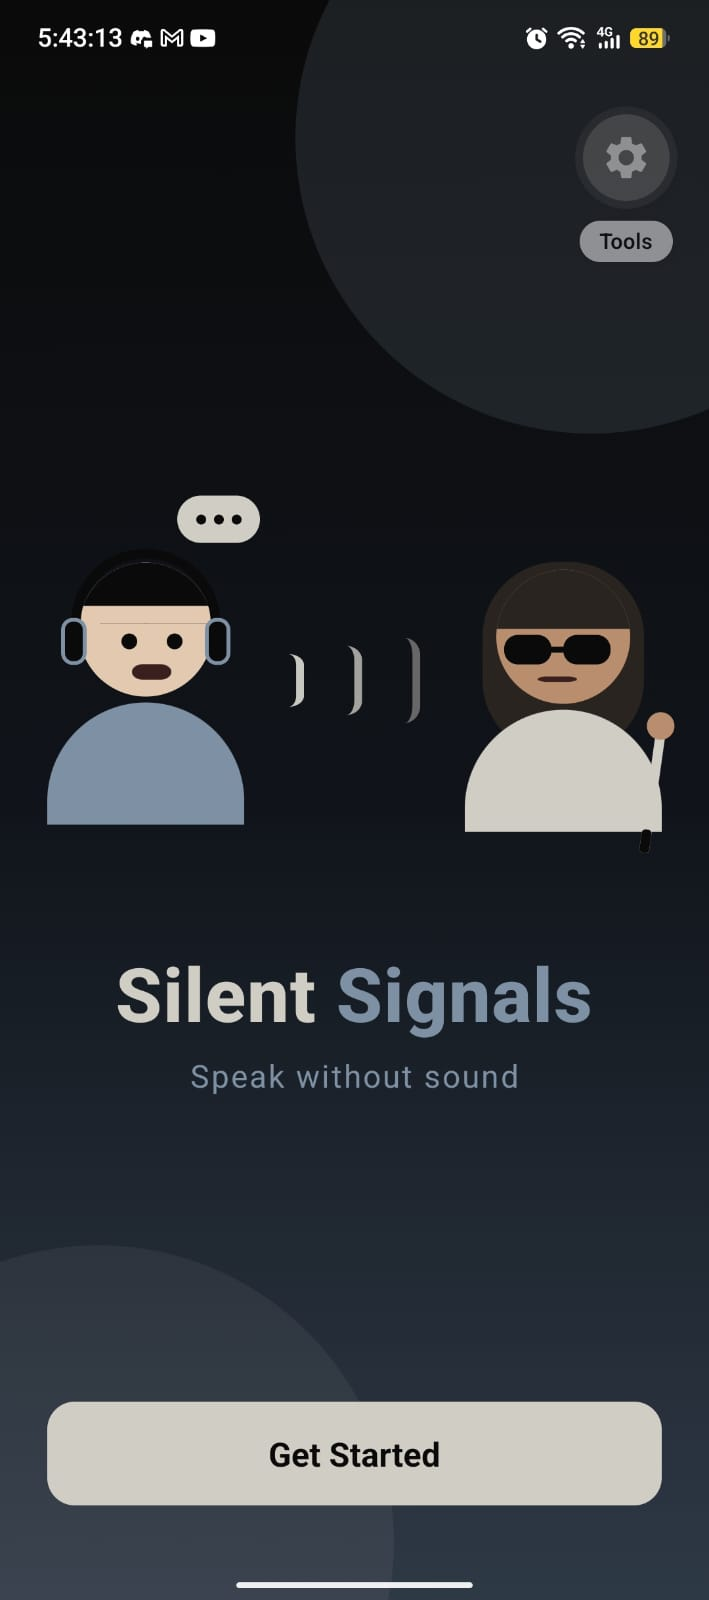
\includegraphics[width=\textwidth]{images/start2.jpeg}
        \caption{First person speaking}
        \label{fig:image1}
    \end{subfigure}
    \hfill
    \begin{subfigure}{0.30\textwidth}
        \centering
        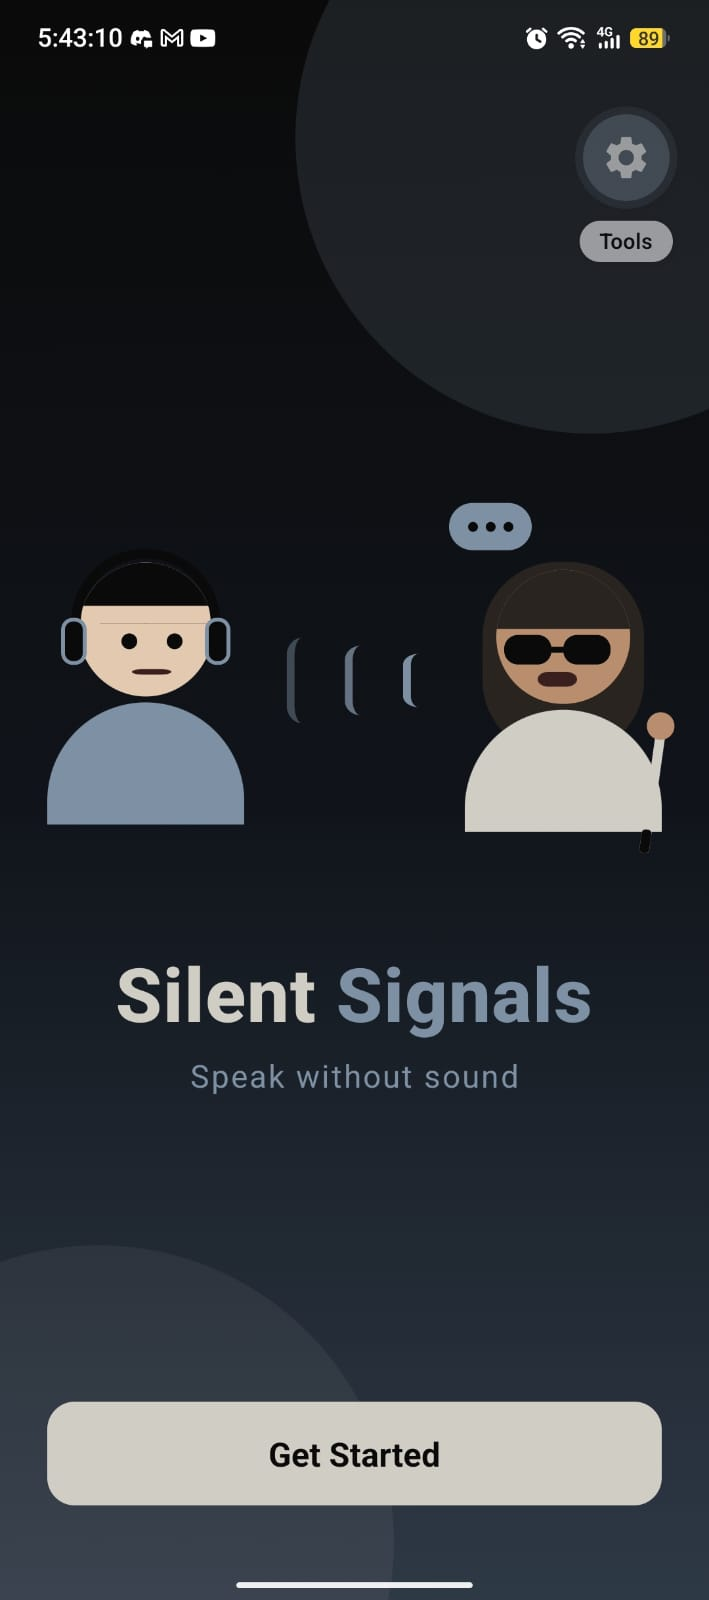
\includegraphics[width=\textwidth]{images/start1.jpeg}
        \caption{Second person speaking}
        \label{fig:image2}
    \end{subfigure}

    \caption{Opening Animations}
    \label{fig:both-images}

    \par\medskip
    Showcases the opening animation of the app.
\end{figure}

\begin{figure}[H]    
    \centering
    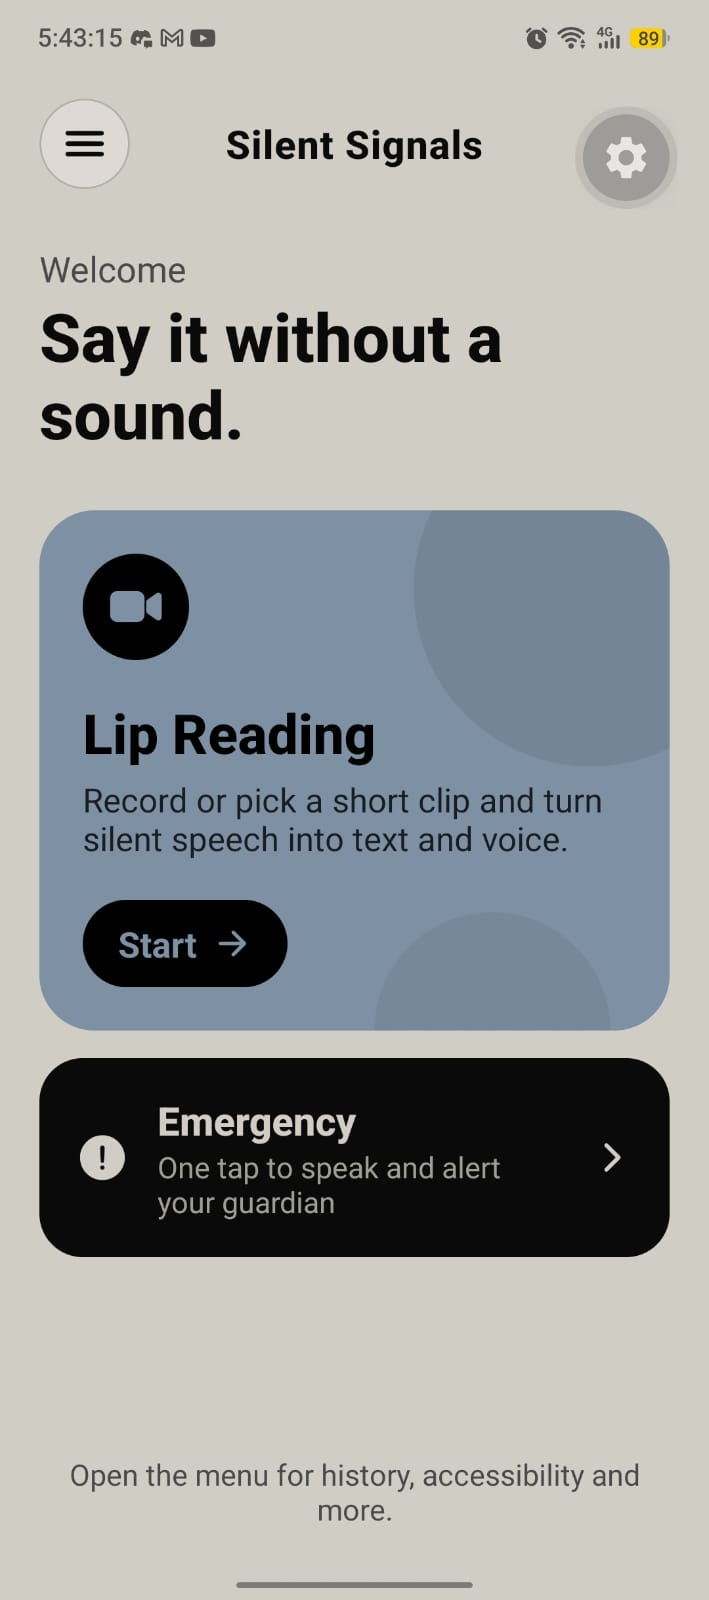
\includegraphics[width=0.30\textwidth]{images/main1.jpeg}
    \caption{Main Screen}
    \label{fig:Profile screen}

    \par\medskip
    Showcases main screen of the app, the user can choose what to do.
\end{figure}



\begin{figure}[H]
    \centering

    \begin{subfigure}{0.30\textwidth}
        \centering
        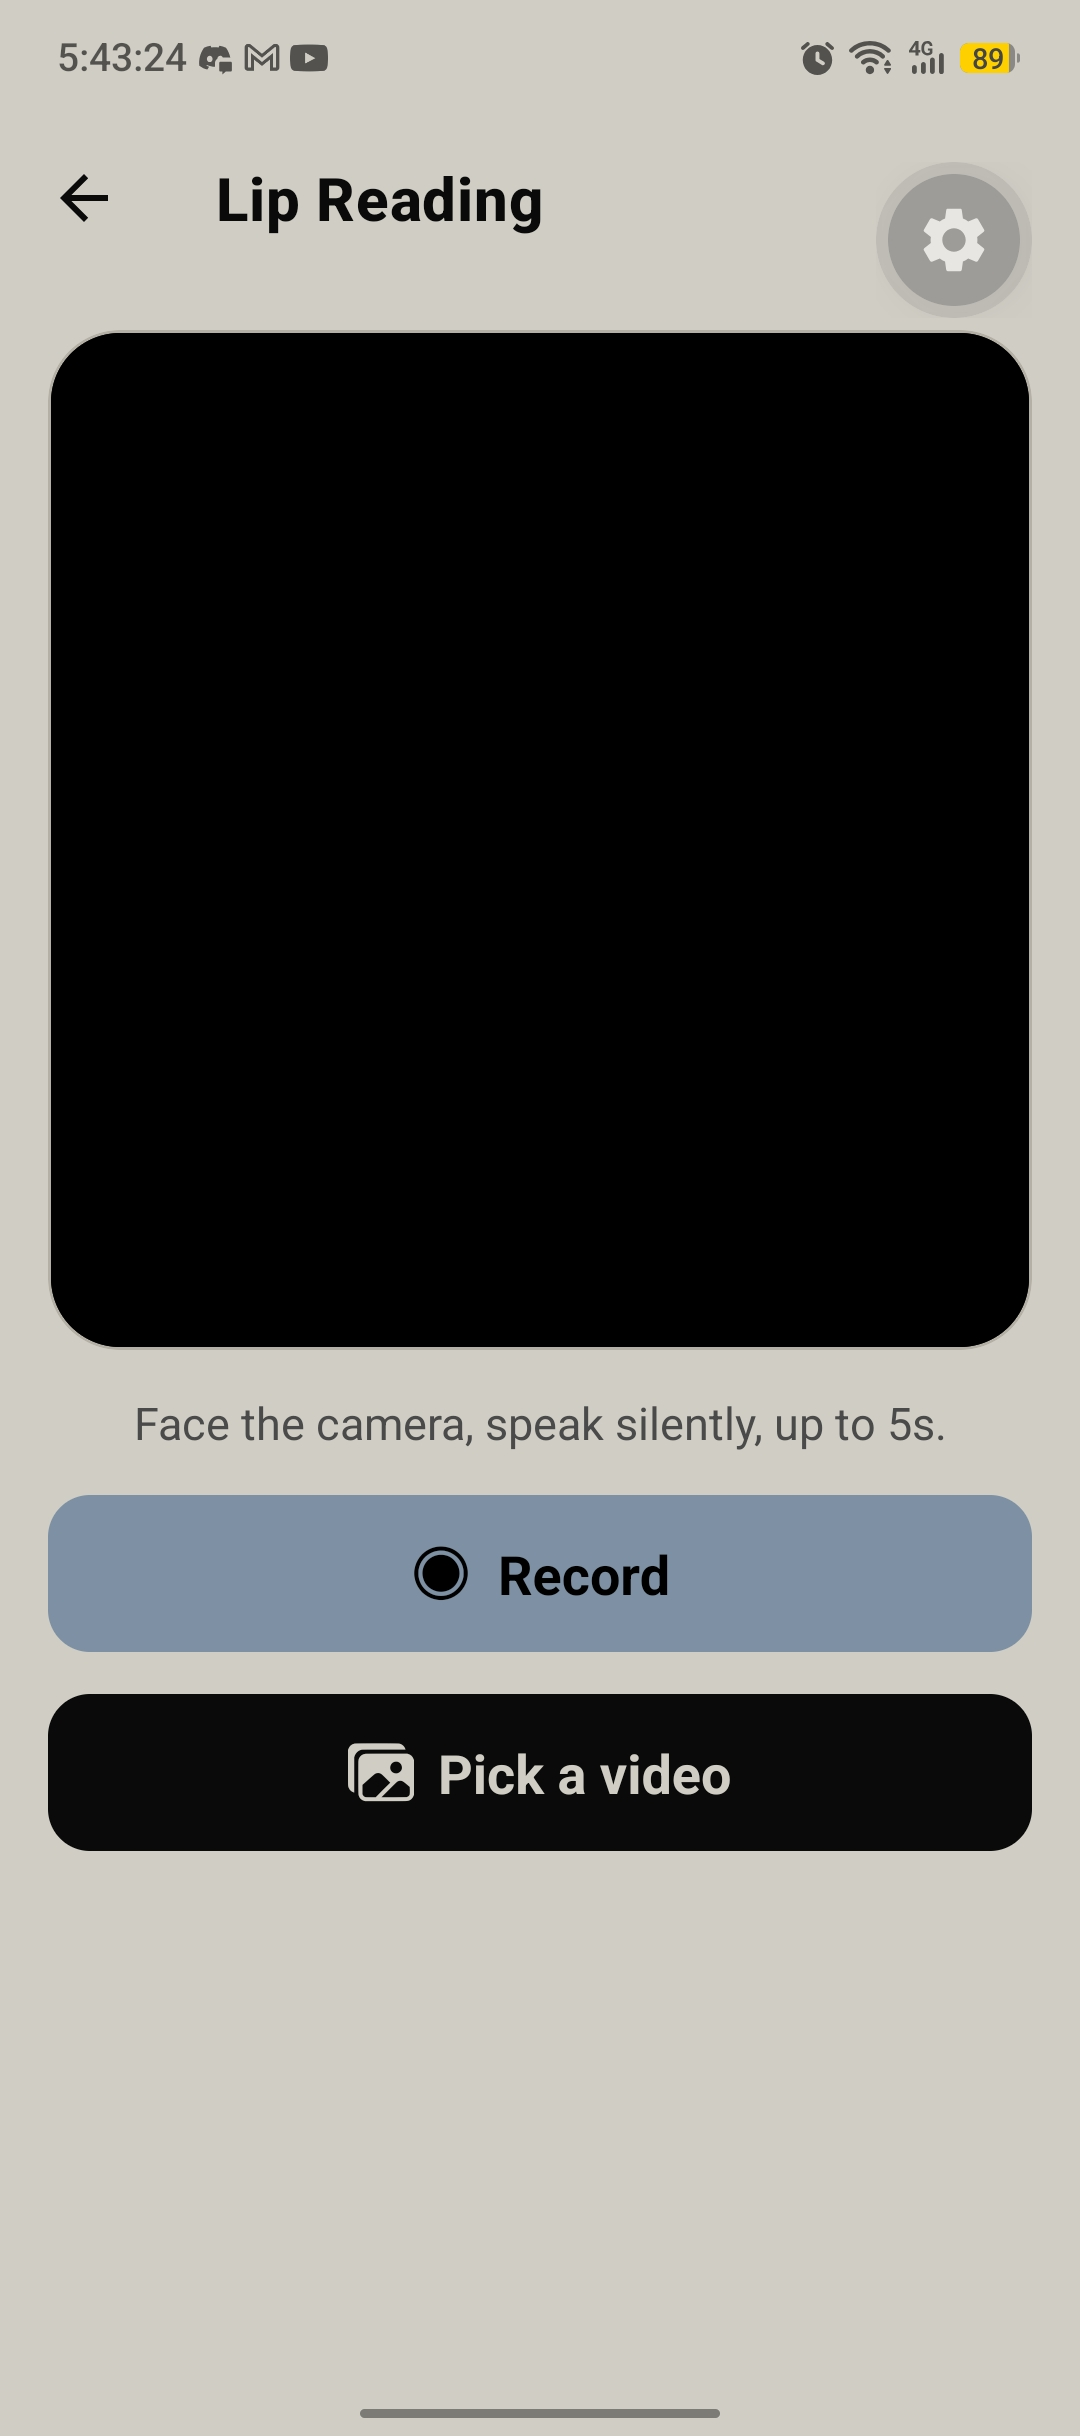
\includegraphics[width=\textwidth]{images/lipreading.jpeg}
        \caption{Lip-Reading Screen}
        \label{fig:image1}
    \end{subfigure}
    \hfill
    \begin{subfigure}{0.30\textwidth}
        \centering
        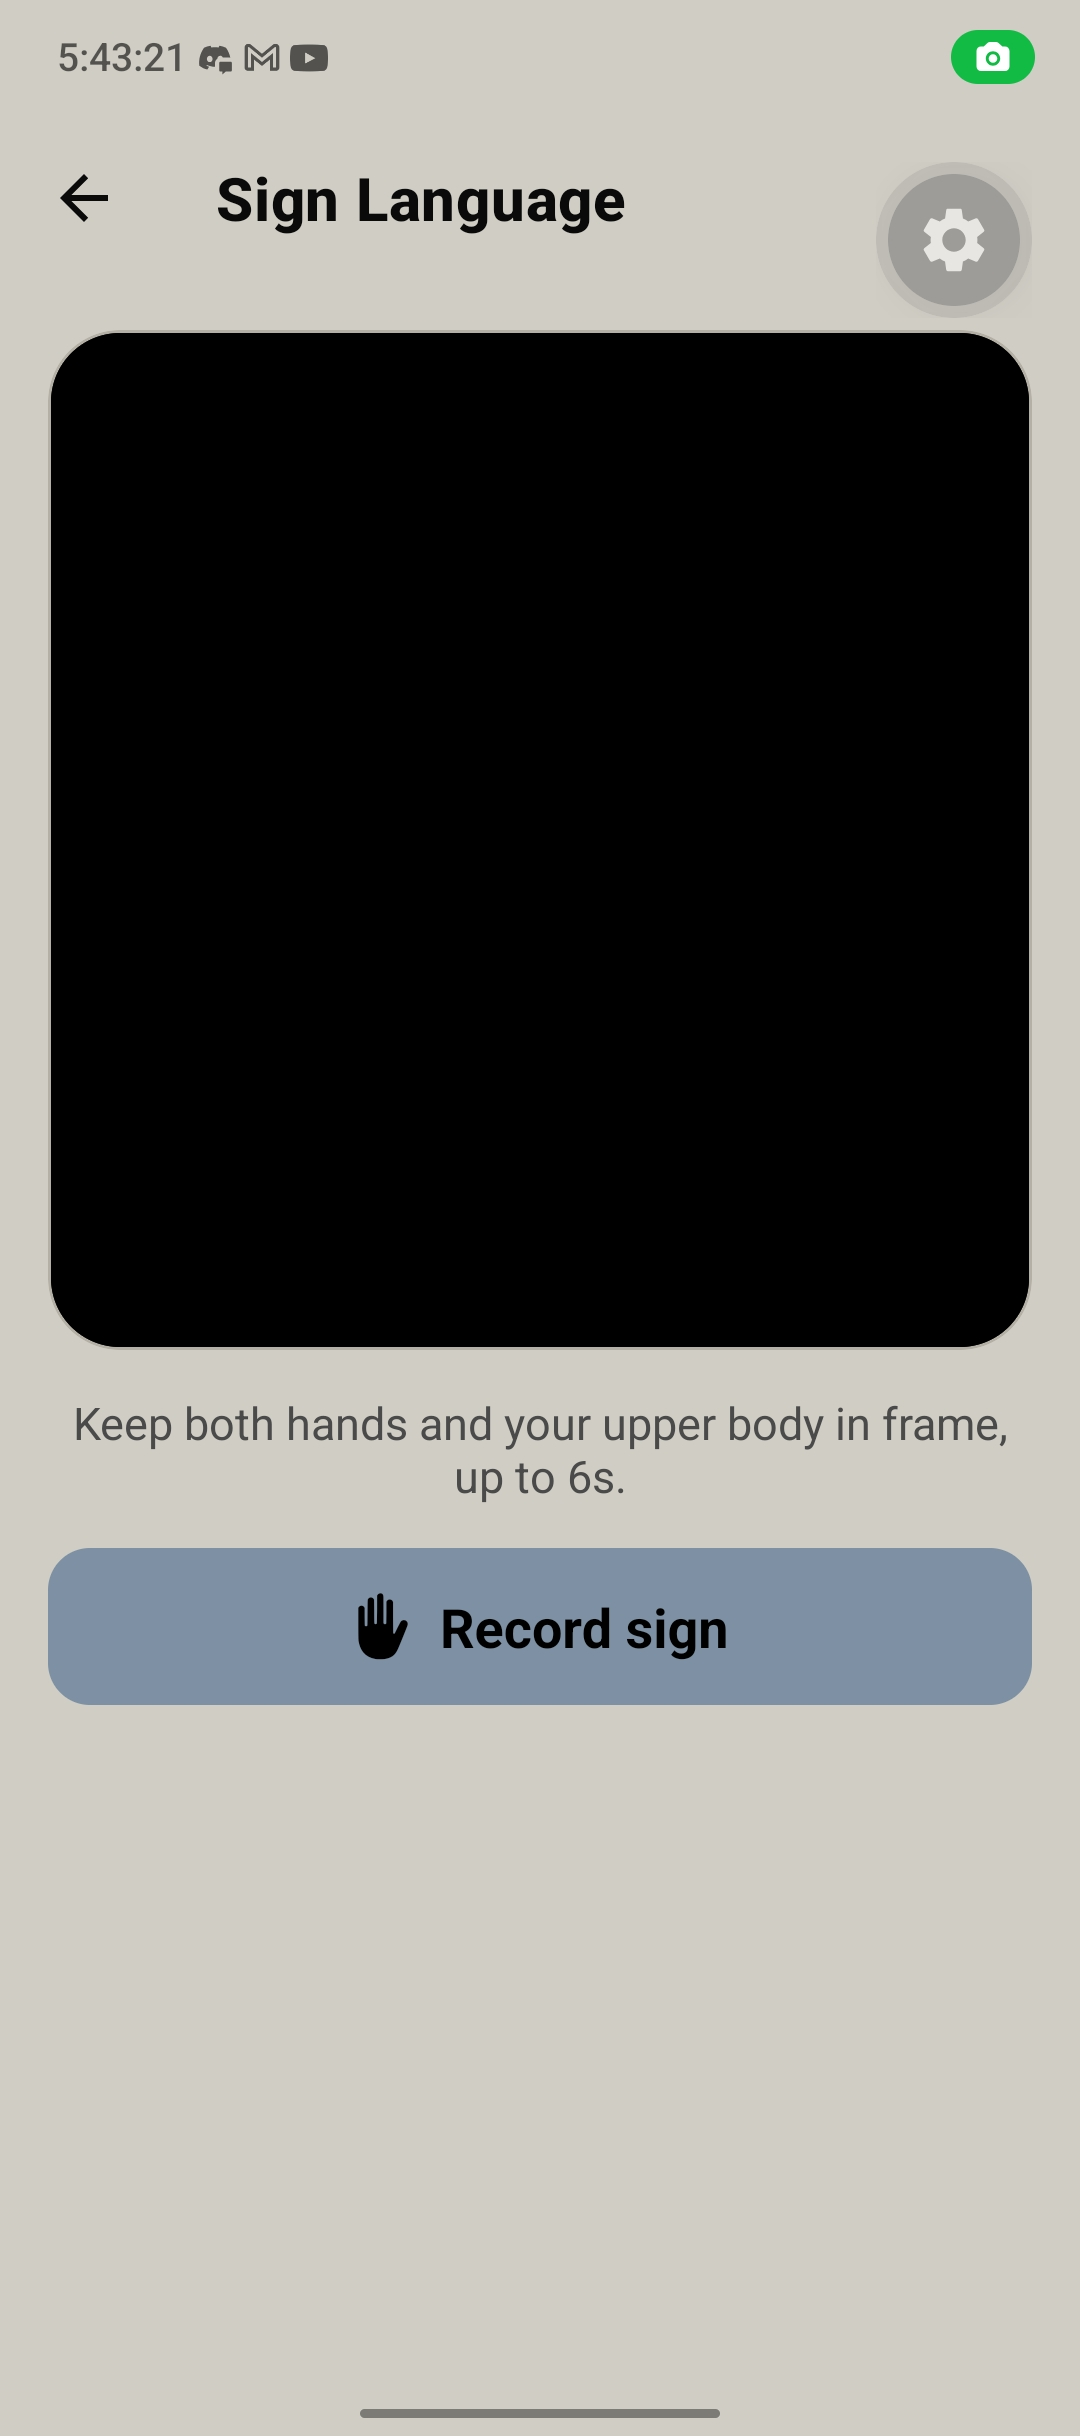
\includegraphics[width=\textwidth]{images/signlanguage.jpeg}
        \caption{Sign Language Detection Screen}
        \label{fig:image2}
    \end{subfigure}

    \caption{Lip-reading and Sign Language Screens}
    \label{fig:both-images}

    \par\medskip
    Showcases the Lip-reading and Sign Language screens of the app.
\end{figure}


\begin{figure}[H]
    \centering

    \begin{subfigure}{0.30\textwidth}
        \centering
        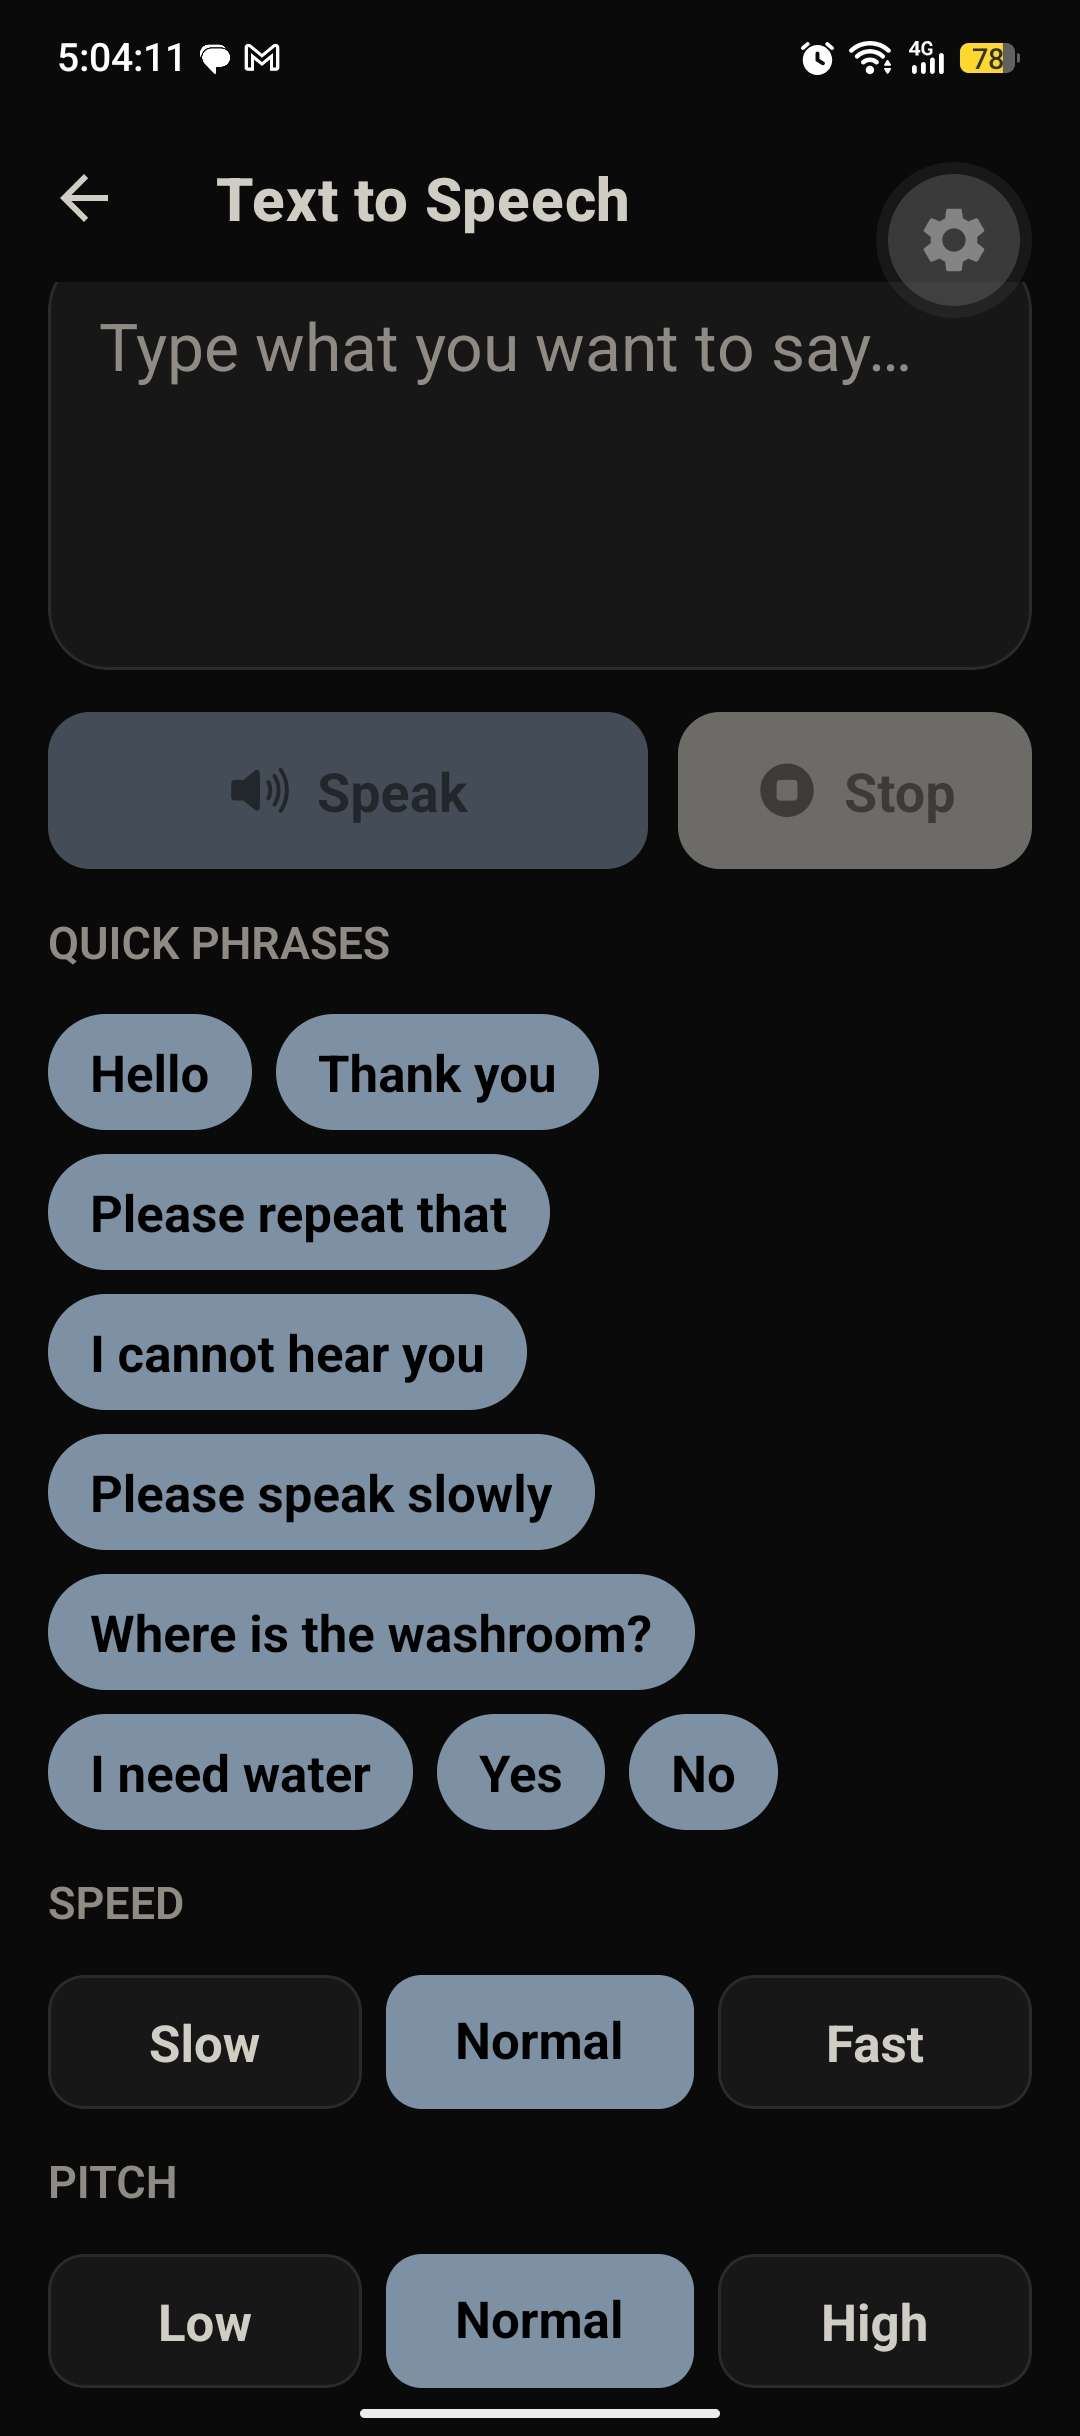
\includegraphics[width=\textwidth]{images/text_to_speech.jpg}
        \caption{Text-To-Speech Screen}
        \label{fig:image1}
    \end{subfigure}
    \hfill
    \begin{subfigure}{0.30\textwidth}
        \centering
        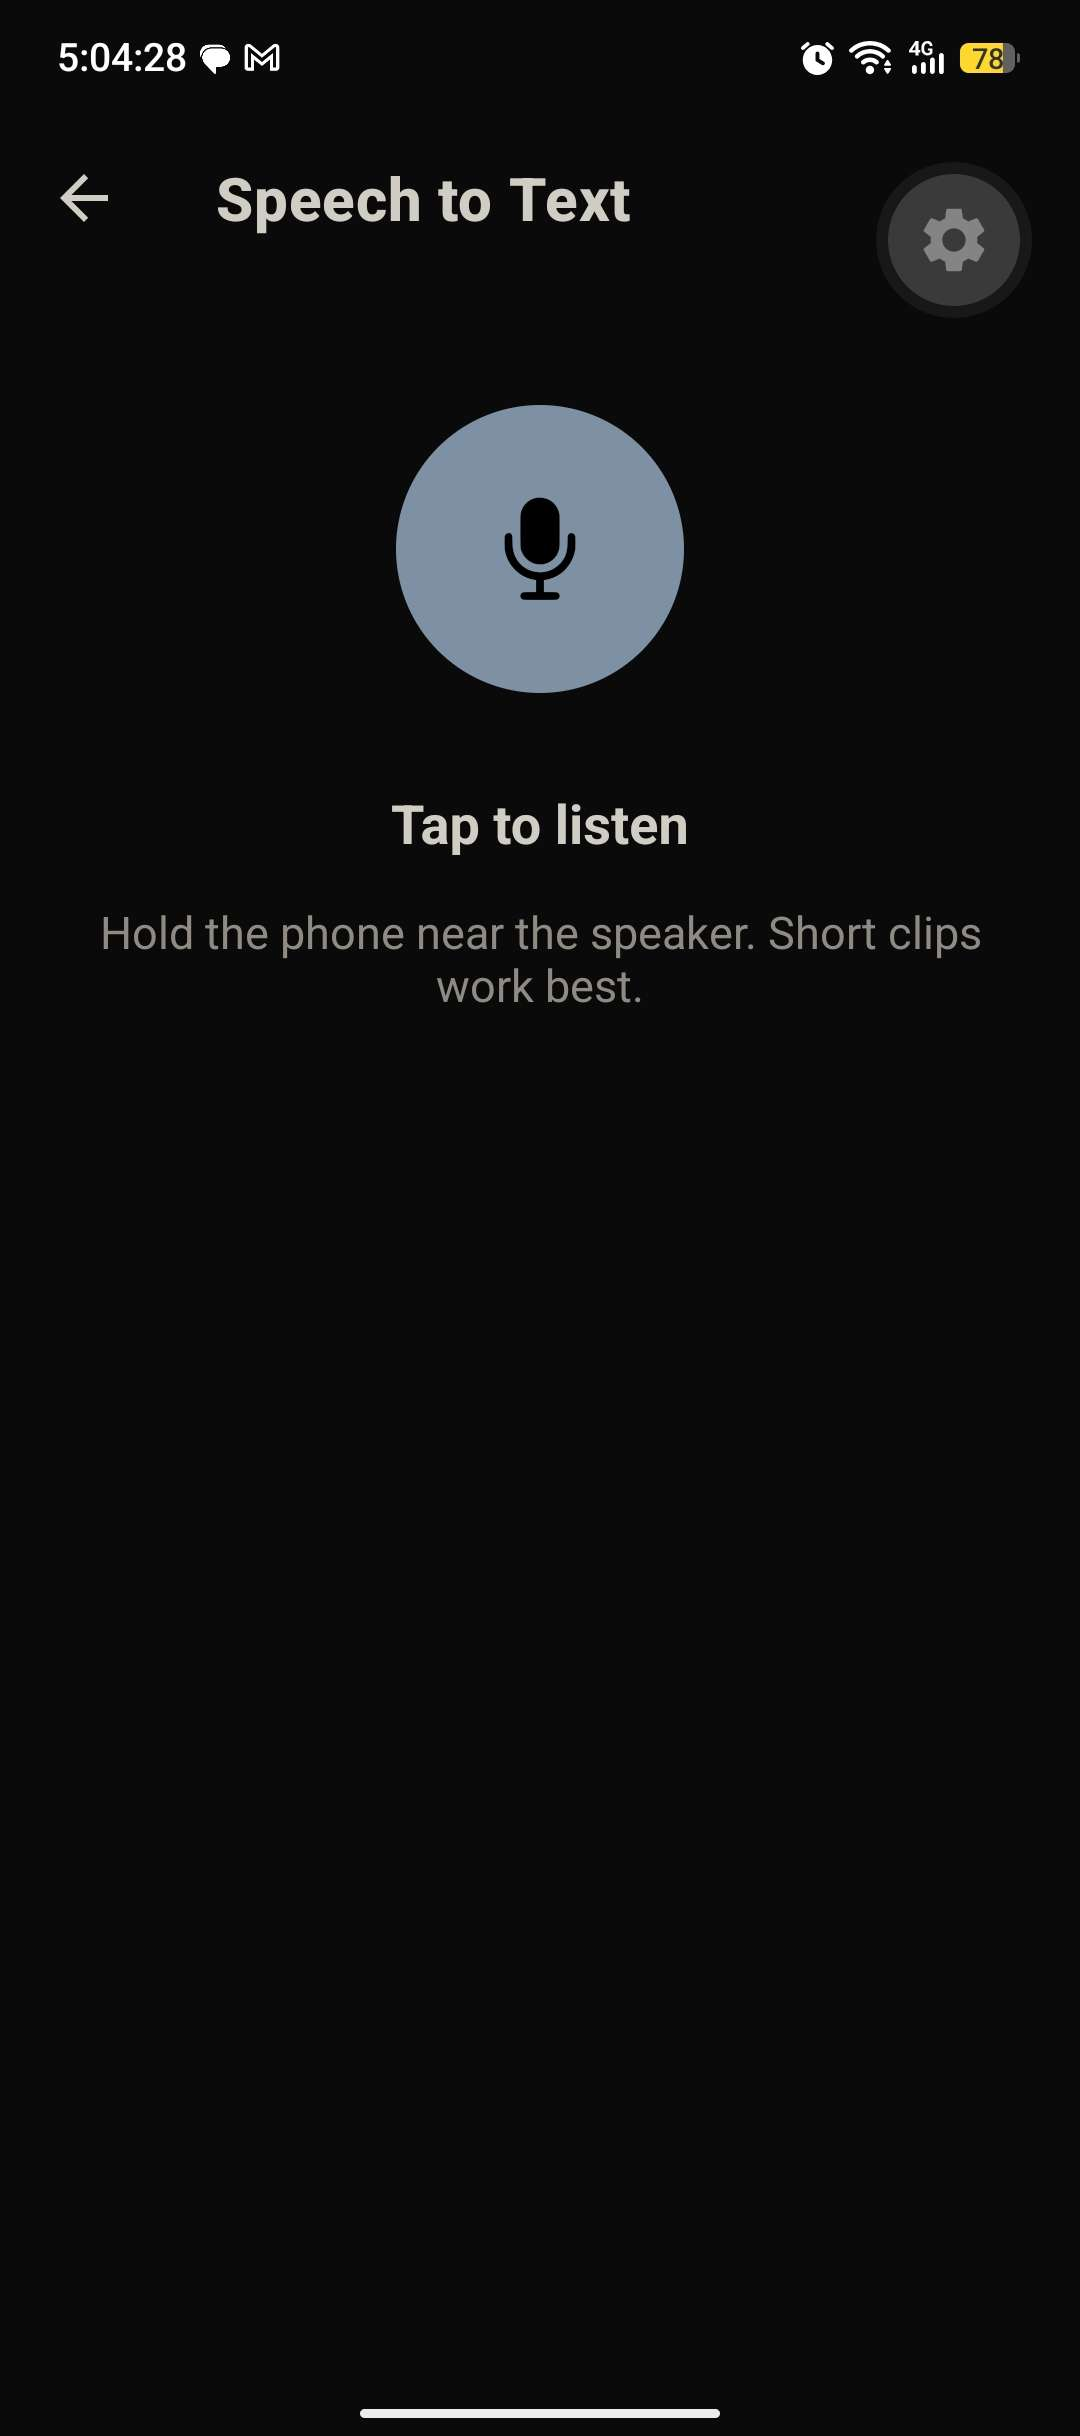
\includegraphics[width=\textwidth]{images/speech_to_text.jpg}
        \caption{Speech-To-Text Screen}
        \label{fig:image2}
    \end{subfigure}

    \caption{Text-To-Speech and Speech-To-Text Screens}
    \label{fig:both-images}

    \par\medskip
    Showcases the Text-To-Speech and Speech-To-Text screens of the app.
\end{figure}

\begin{figure}[H]
    \centering

    \begin{subfigure}{0.30\textwidth}
        \centering
        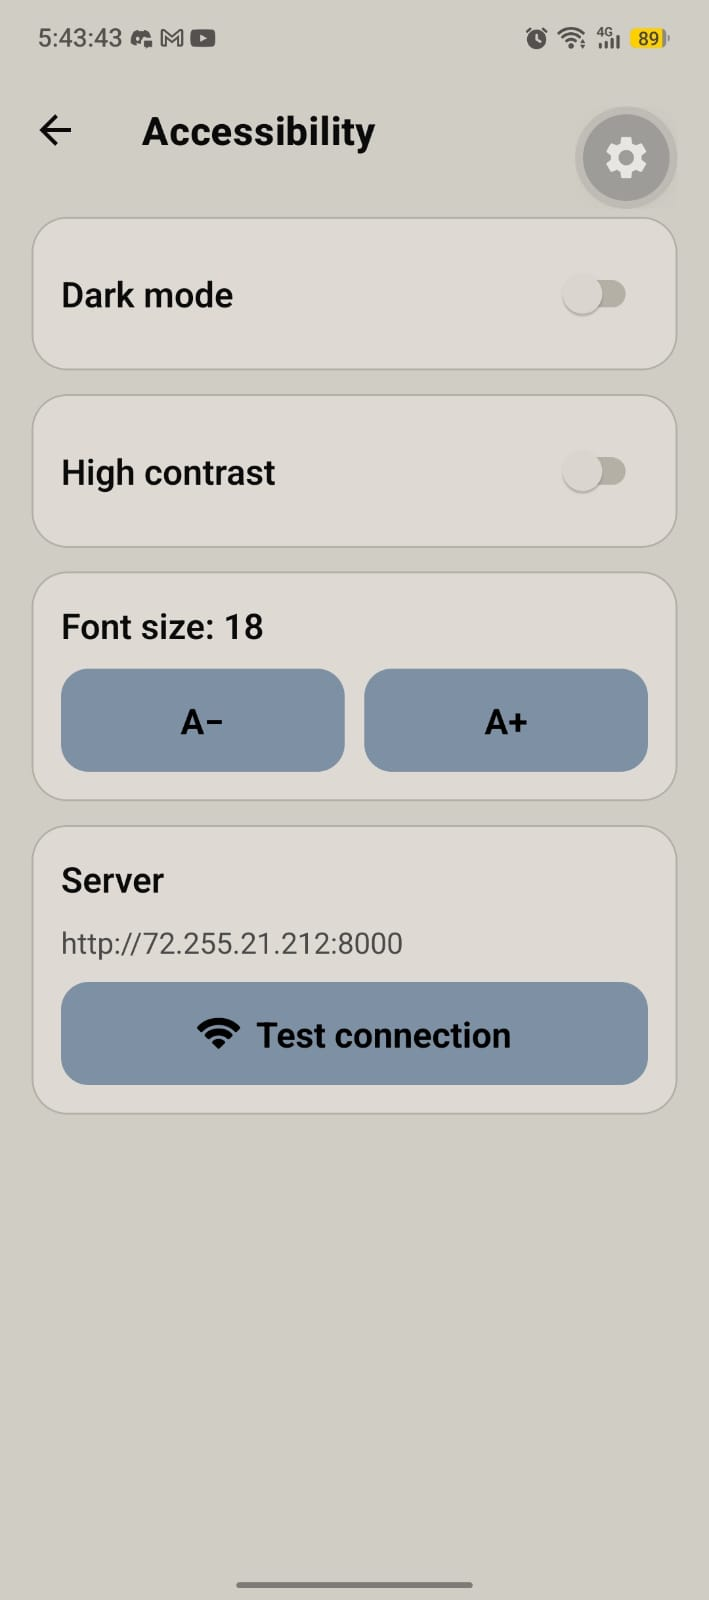
\includegraphics[width=\textwidth]{images/accessibility.jpeg}
        \caption{Accessibility Settings Screen}
        \label{fig:image1}
    \end{subfigure}
    \hfill
    \begin{subfigure}{0.30\textwidth}
        \centering
        
\includegraphics[width=\textwidth]{images/history.jpeg}
        \caption{User Conversation History Screen}
        \label{fig:image2}
    \end{subfigure}

    \caption{Accessibility Settings and User Conversation History Screens}
    \label{fig:both-images}

    \par\medskip
    Showcases the Accessibility Settings and User Conversation History screens of the app.
\end{figure}


\begin{figure}[H]    
    \centering
    \begin{subfigure}{0.30\textwidth}
        \centering
        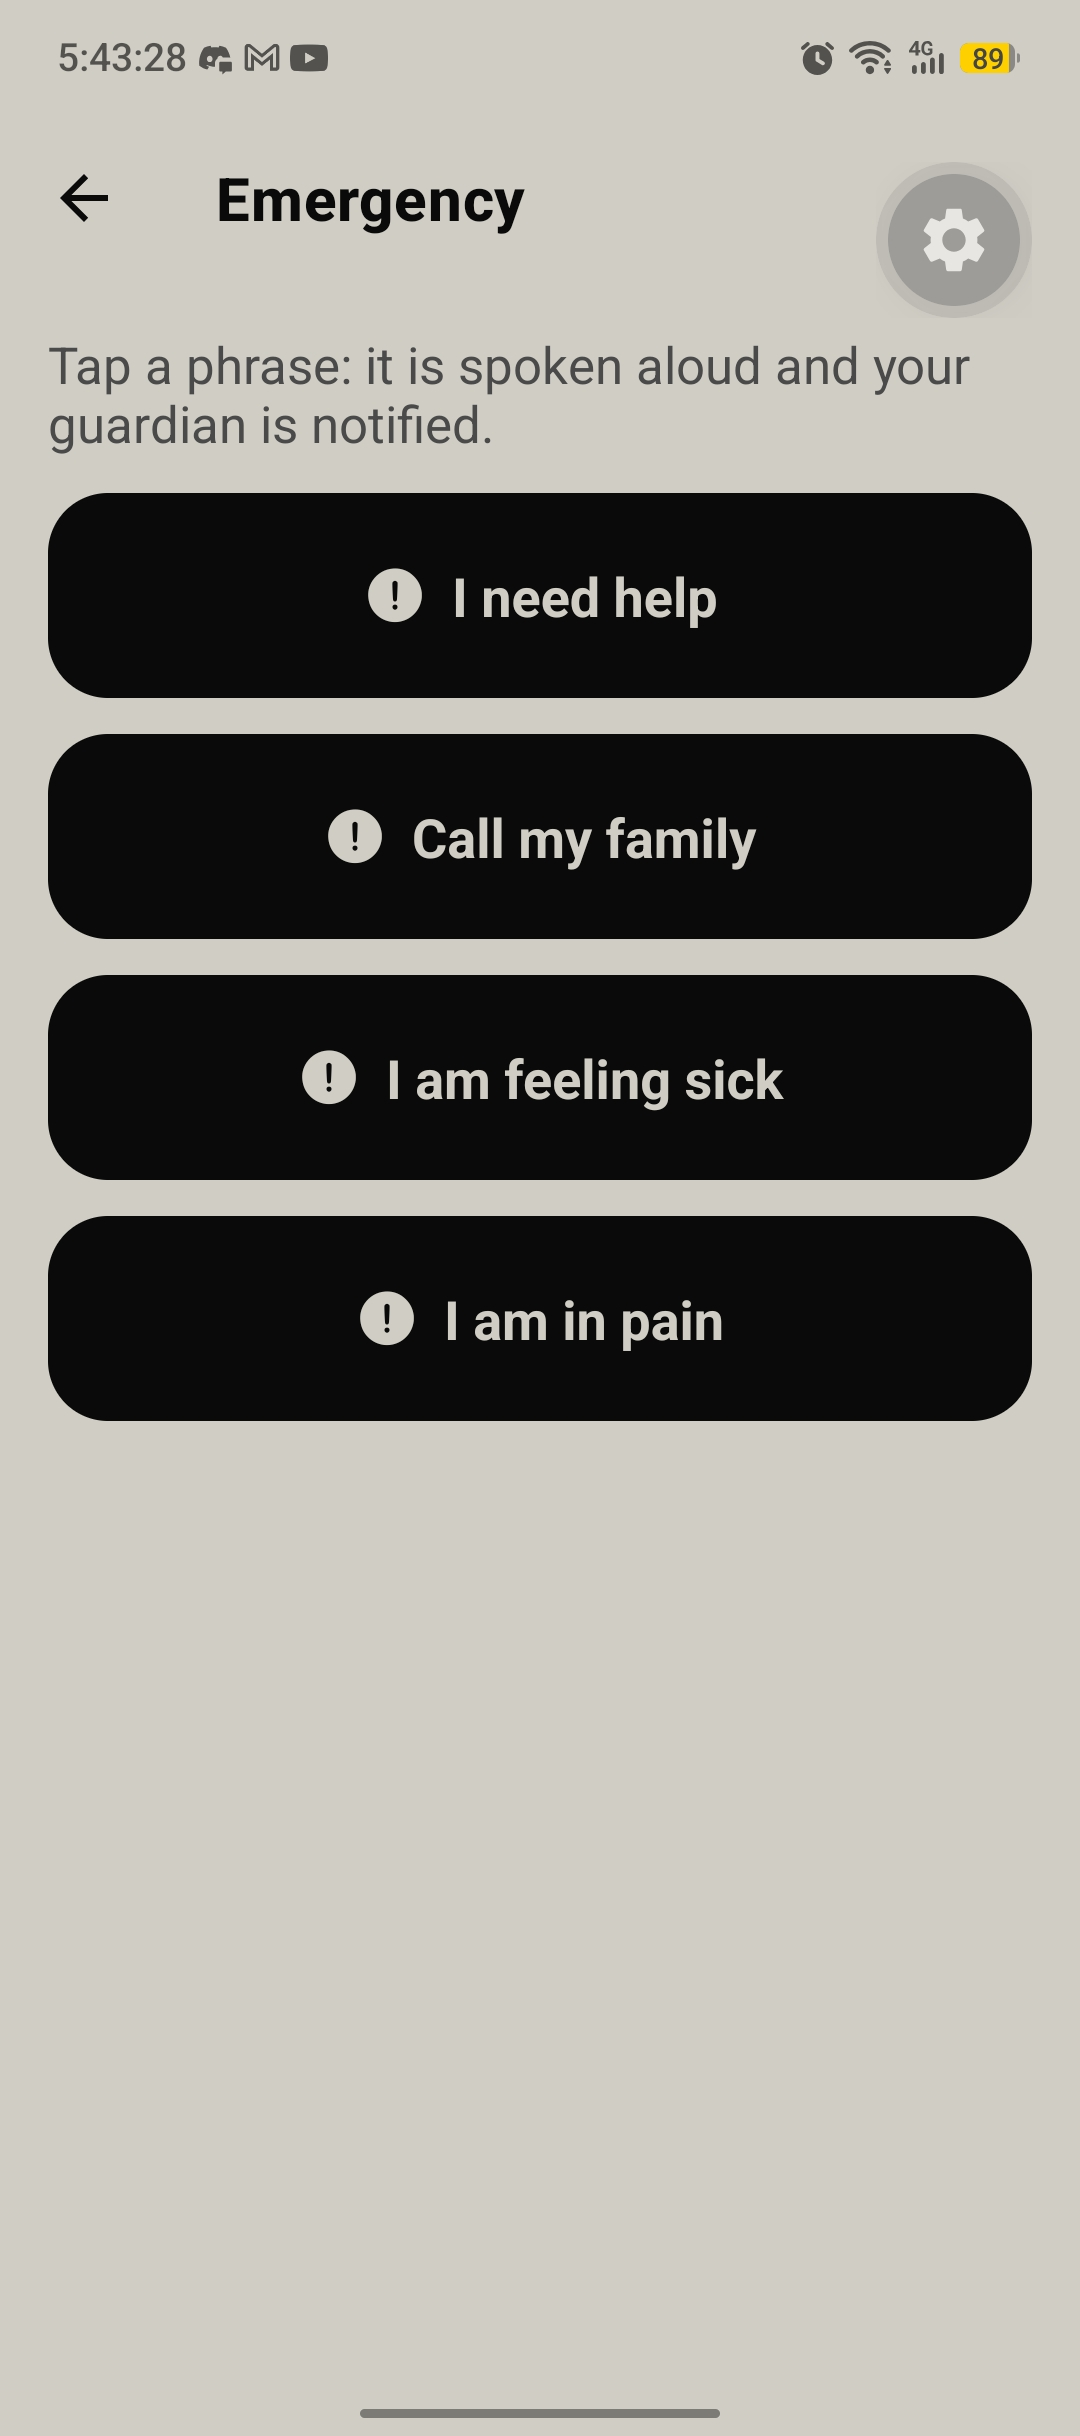
\includegraphics[width=\textwidth]{images/emergency.jpeg}
        \caption{Emergency Phrases Screen}
        \label{fig:image1}
    \end{subfigure}
    \hfill
    \begin{subfigure}{0.30\textwidth}
        \centering
        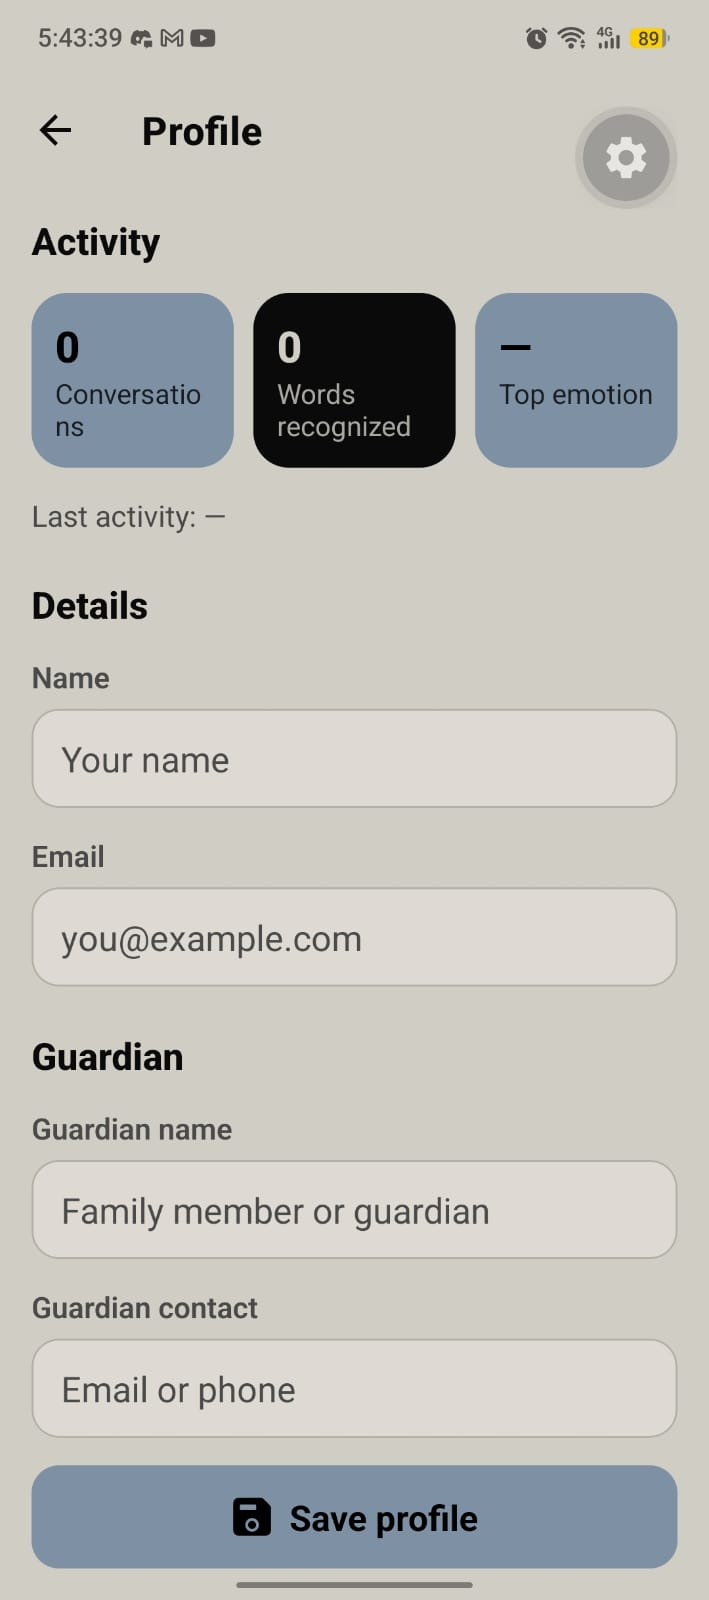
\includegraphics[width=\textwidth]{images/profile.jpeg}
        \caption{User Profile Screen}
        \label{fig:gui-profile}
    \end{subfigure}

    \caption{Emergency Phrases and User Profile Screens}
    \label{fig:gui-emergency}

    \par\medskip
    Showcases the Emergency Phrases and local User Profile Screen on the app.
\end{figure}



\section{Database Design }
\subsection{ER Diagram}
The Entity-Relationship (ER) diagram provides a detailed representation of the database design for our system. It encompasses various entities, each of which plays a crucial role in the system’s functionality. These entities include:
\begin{itemize}
  \item Users: This entity stores the basic information of registered users, including their name, email, password, and unique UserID.
  \item EmergencyWords: This entity stores emergency-related words or phrases configured for each user. These words are used to identify potential emergency situations.
  \item Settings: This entity stores user-specific configuration preferences, such as font size, dark mode, and font contrast, allowing the system to provide a personalized and accessible experience.
  \item ConversationHistory: This entity maintains records of the user's conversations, including the conversation ID, source, raw text, corrected text, and detected emotion. It allows previous interactions to be stored and referenced.
  \item Guardians: This entity stores information about the emergency contacts associated with a user, including the guardian's name, contact information, communication medium, and unique GuardianID.
  \item EmergencyHistory: This entity maintains a record of detected emergency events. It stores information such as the event ID, associated user and guardian, detected emergency phrase, and the time at which the event occurred.
\end{itemize}
Each of these entities interacts with others to support the core functionality of the system. Users can configure their Settings, define EmergencyWords, and have associated Guardians. The system stores their ConversationHistory, while detected emergency situations are recorded in EmergencyHistory and can trigger notifications to the user's designated guardians. The ER diagram therefore serves as a roadmap for understanding the database structure, relationships, and overall data flow of the system.

\begin{figure}[H]    
    \centering
    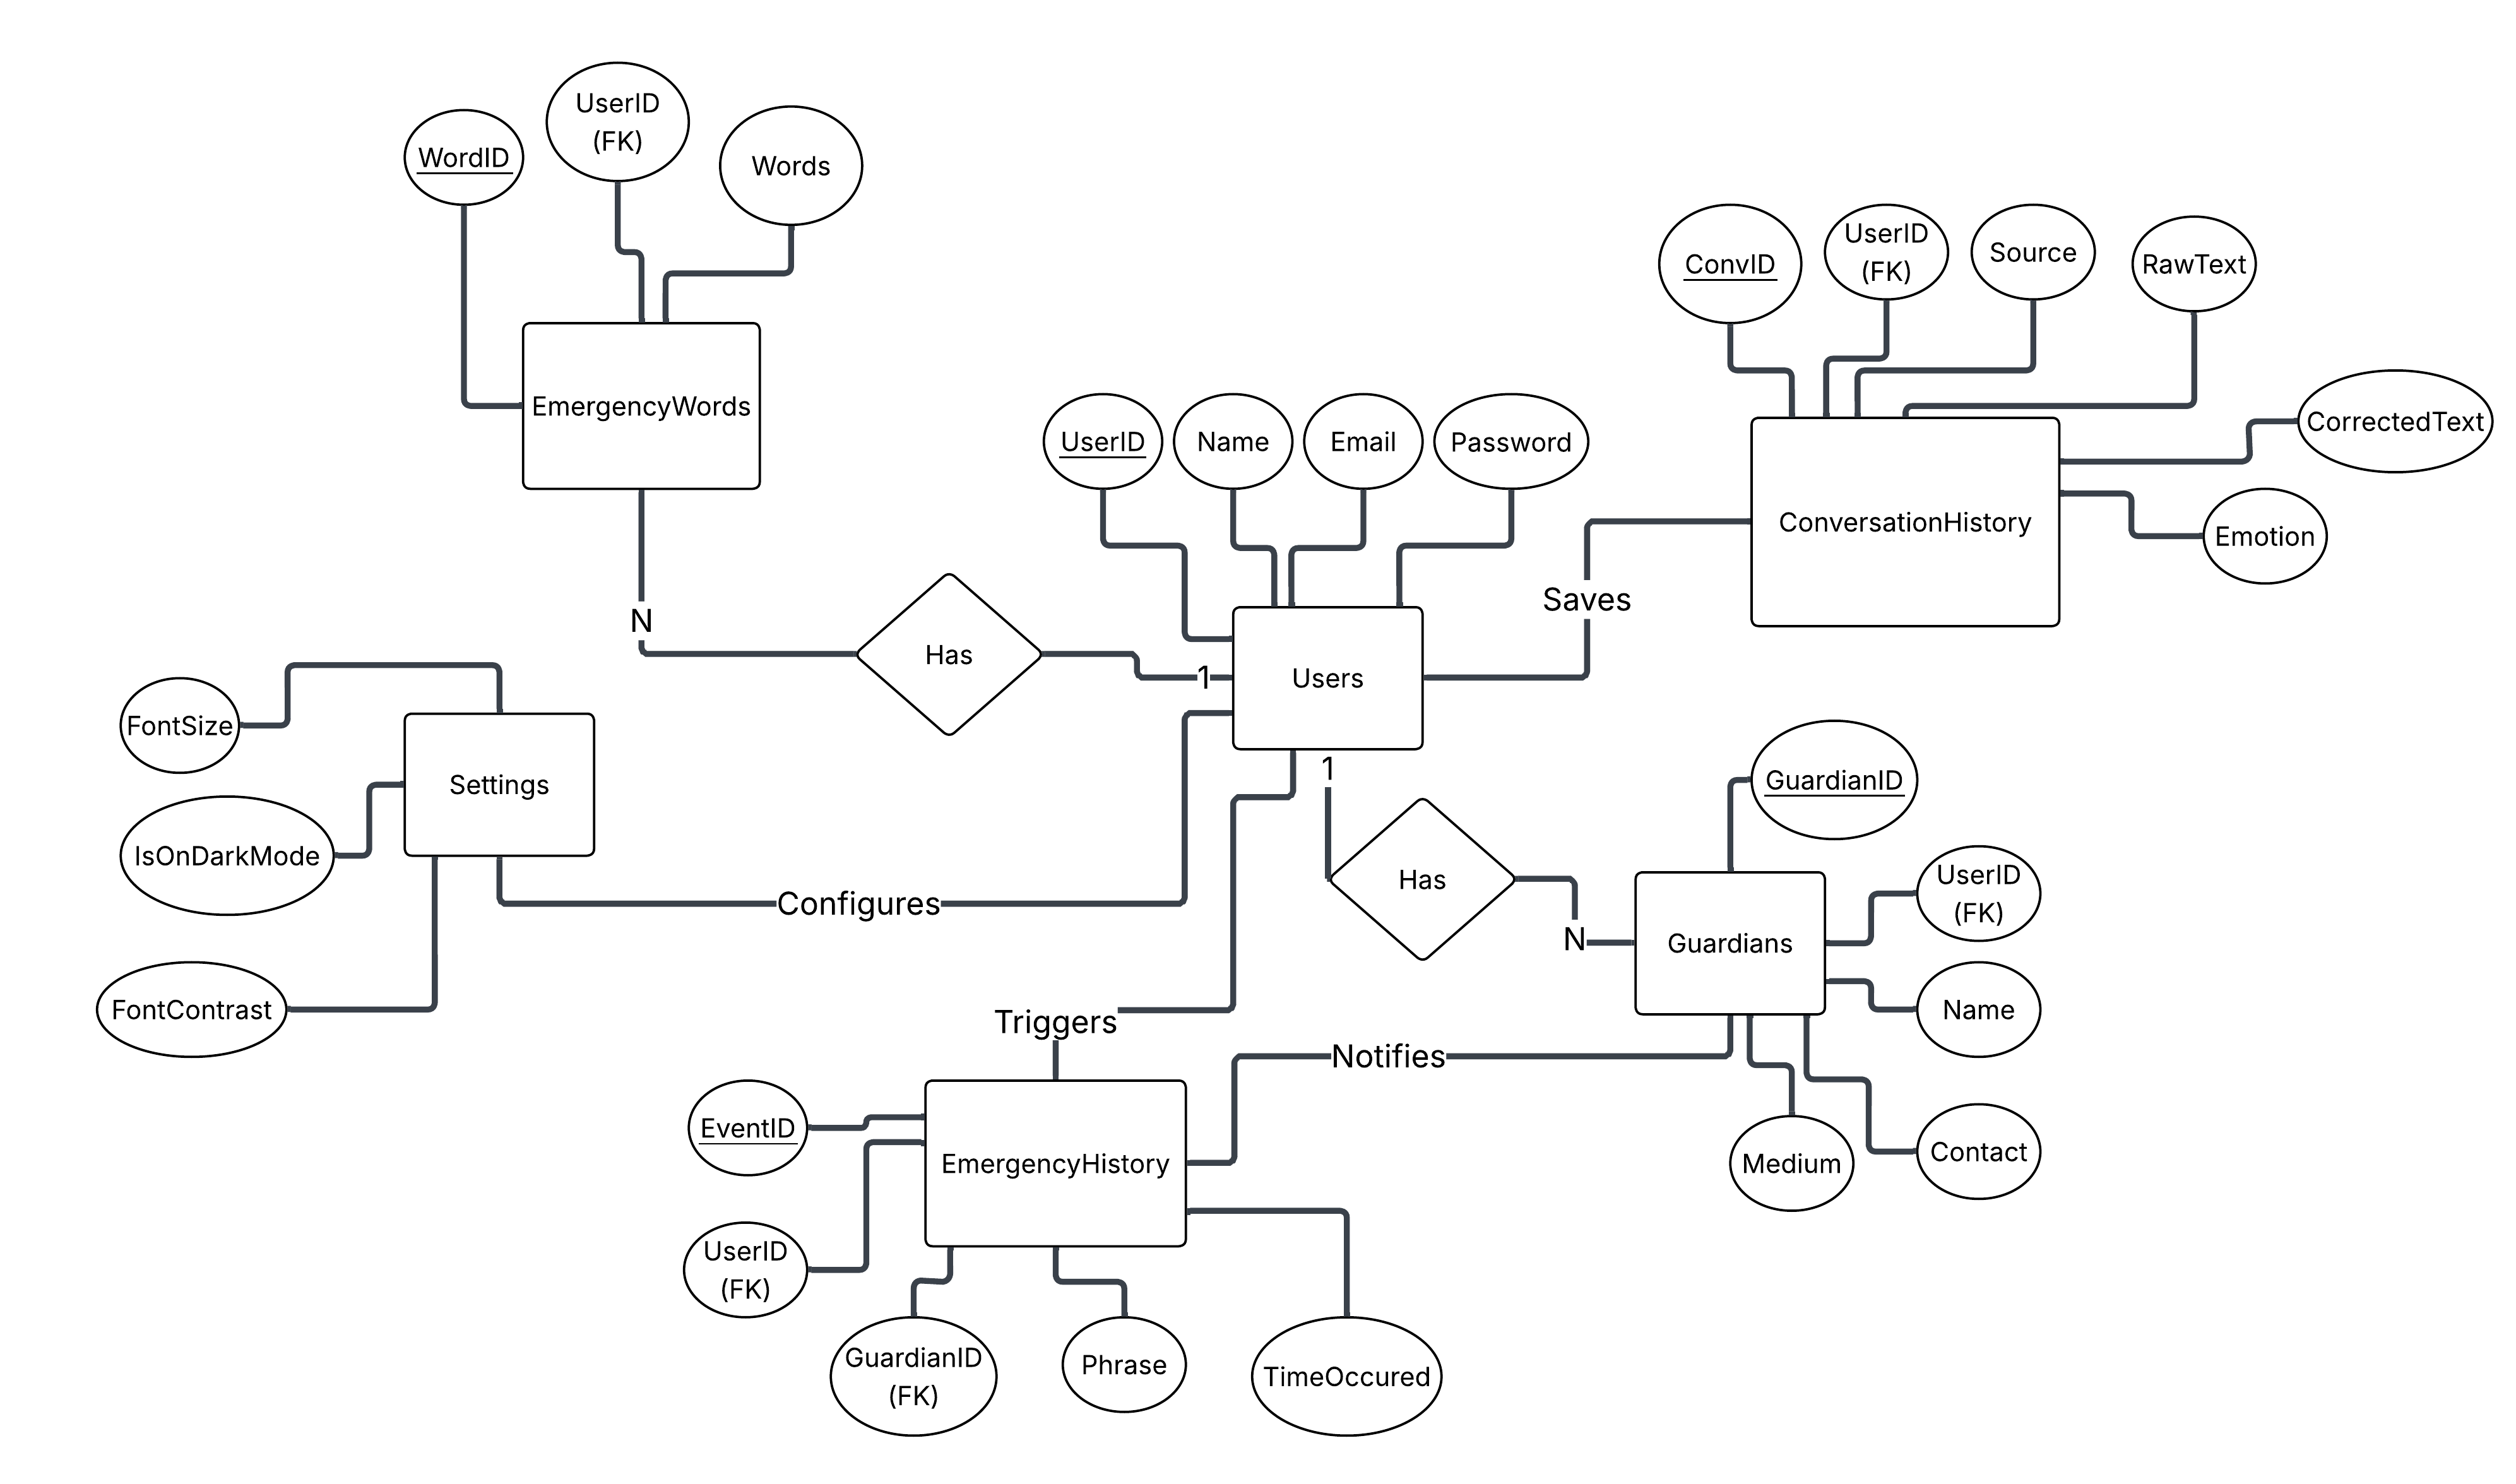
\includegraphics[width=\textwidth]{images/db diagram.png}
    \caption{Entity Relationship Diagram}
    \label{fig:Profile screen}
\end{figure}


\subsection{Data Dictionary}
Data dictionary given below defines all the entities, their attributes and data-types.
\renewcommand{\arraystretch}{1.3}
\begin{xltabular}{\textwidth}{|>{\centering\arraybackslash}p{2.4cm}|p{2.3cm}|p{2.7cm}|p{1.9cm}|p{1.5cm}|X|}
\caption{Database schema}
\label{tab:schema} \\
\hline
\textbf{Entity} & \textbf{Attribute} & \textbf{Datatype} & \textbf{Relation To} & \textbf{Nullable} & \textbf{Description} \\ \hline
\endfirsthead

\hline
\textbf{Entity} & \textbf{Attribute} & \textbf{Datatype} & \textbf{Relation To} & \textbf{Nullable} & \textbf{Description} \\ \hline
\endhead

\hline
\endfoot

% ---------- Users ----------
\textbf{Users} & \textbf{UserID} & UniqueIdentifier & & No & Primary Key of Users table \\ \cline{2-6}
 & Name & String & & No & Name of the user \\ \cline{2-6}
 & Email & String & & No & Email address of the user \\ \cline{2-6}
 & Password & String & & No & Password of the user \\ \hline

% ---------- EmergencyWords ----------
\textbf{Emergency\newline Words} & \textbf{WordID} & UniqueIdentifier & & No & Primary Key of EmergencyWords table \\ \cline{2-6}
 & UserID & UniqueIdentifier & Users & No & Foreign Key referencing the user associated with the emergency word \\ \cline{2-6}
 & Words & String & & No & Emergency word or phrase configured by the user \\ \hline

% ---------- ConversationHistory ----------
\textbf{Conversation\newline History} & \textbf{ConvID} & UniqueIdentifier & & No & Primary Key of ConversationHistory table \\ \cline{2-6}
 & UserID & UniqueIdentifier & Users & No & Foreign Key referencing the user who participated in the conversation \\ \cline{2-6}
 & Source & String & & No & Source or input modality of the conversation \\ \cline{2-6}
 & RawText & String & & No & Original text generated or received from the conversation \\ \cline{2-6}
 & CorrectedText & String & & No & Corrected or processed version of the conversation text \\ \cline{2-6}
 & Emotion & String & & No & Emotion detected from the conversation \\ \hline

% ---------- Settings ----------
\textbf{Settings} & FontSize & Integer & & No & Font size selected by the user \\ \cline{2-6}
 & IsOnDarkMode & Boolean & & No & Indicates whether dark mode is enabled \\ \cline{2-6}
 & FontContrast & Integer & & No & Font contrast setting selected by the user \\ \hline

% ---------- Guardians ----------
\textbf{Guardians} & \textbf{GuardianID} & UniqueIdentifier & & No & Primary Key of Guardians table \\ \cline{2-6}
 & UserID & UniqueIdentifier & Users & No & Foreign Key referencing the user associated with the guardian \\ \cline{2-6}
 & Name & String & & No & Name of the guardian \\ \cline{2-6}
 & Medium & String & & No & Communication medium used to notify the guardian \\ \cline{2-6}
 & Contact & String & & No & Contact information of the guardian \\ \hline

% ---------- EmergencyHistory ----------
\textbf{Emergency\newline History} & \textbf{EventID} & UniqueIdentifier & & No & Primary Key of EmergencyHistory table \\ \cline{2-6}
 & UserID & UniqueIdentifier & Users & No & Foreign Key referencing the user associated with the emergency event \\ \cline{2-6}
 & GuardianID & UniqueIdentifier & Guardians & No & Foreign Key referencing the guardian associated with the emergency notification \\ \cline{2-6}
 & Phrase & String & & No & Emergency phrase that triggered the event \\ \cline{2-6}
 & TimeOccured & DateTime & & No & Date and time when the emergency event occurred \\ \hline
\end{xltabular}



\section{ Risk Analysis}
Three major risks are associated with this project, which are Time, Performance and Data constraints.\\
The project involves various phases like dataset collection (public datasets for lip reading, sign language and facial expressions), data pre-processing, model training, testing, model integration and front-end implementation. The system also includes many modules, such as the language model correction, emotion detection, the Sound Optimizer, the emergency notifier and the performance dashboard. Given the amount of work, time is a major constraint that needs to be managed carefully during the project.
Next is performance. Because this project aims to let users hold a normal conversation without an interpreter, a wrong or slow prediction can lead to misunderstanding, especially in an emergency. Lip reading is a difficult problem, and the system has to run in real time on a standard webcam and consumer hardware while remaining accurate enough to be useful. Thus, performance constraints also pose a major risk.
Finally, there is data. Lip-reading and sign language models depend heavily on the quality and size of the training datasets, and most public datasets cover limited vocabularies, specific speakers and controlled lighting. Models trained on them may not perform as well on real users in everyday conditions, so limited or unsuitable data poses a further risk to accuracy.

\chapter{Proposed Approach and Methodology}
\label{ch:approach}
This chapter presents the proposed approach and methodology for the development of Silent Signals. The system is built as a set of modules that share a common pipeline: video from the camera is passed through a landmark detector, the relevant region of the face or body is passed to a recognition model, the recognised words are corrected by a language model and shown with a confidence score, and the confirmed sentence can then be spoken aloud. The chapter describes the three modules that have been designed in detail in FYP-I, namely the lip-reading module, the sign language module and the context based correction module. For the lip-reading module it describes the data collection, the pre-processing of the video and the details of the model, and for the other two modules it describes the models that will be used and the reasons for choosing them. The lip-reading module is described first and in the most detail, because it is the main contribution of the project and the only module that is trained by the team rather than taken from a pretrained source. The choices made in this chapter follow from the literature reviewed in Chapter~\ref{ch:lit}, and the remaining modules, such as speech output, sound optimization and facial expression detection, are placed in the overall architecture in Chapter~\ref{ch:design}.

\section{Lip-Reading Module}
This section describes the lip-reading module, which converts a silent video of a speaker's face, either recorded or from a live webcam, into text. It is the core of Silent Signals, because it gives a person who cannot produce clear speech a way to be understood simply by moving their lips in front of an ordinary camera. The module follows the design that the literature in Chapter~\ref{ch:lit} has shown to work for visual speech recognition: the mouth region is located with facial landmarks and cropped from every frame, the sequence of crops is passed to a spatio-temporal network that captures both the shape of the lips and their movement over time, and the network outputs a probability for every word in its vocabulary. The highest probability becomes the predicted word and is also shown to the user as the confidence score for that word. The module is trained on a public dataset recorded in natural conditions rather than in a studio, so that it has a better chance of working for users who were never seen during training. The following subsections describe the data on which the module is trained and evaluated, the pre-processing that turns raw video into model input, and the architecture of the network itself.

\subsection{Data collection}
The module will be trained and evaluated on the Lip Reading in the Wild (LRW) dataset \cite{ref:Chung:2016}, which is publicly available for research. LRW contains approximately 500 distinct English word classes, with hundreds of video samples for each word collected from television broadcasts. Each clip is a short, word-level video segment in which a speaker articulates the target word, making the dataset suitable for training a model to recognize spoken words using only visual information from the speaker's lips. The videos contain natural variations in speakers, appearance, pose, lighting and speaking style, providing a more realistic setting for visual speech recognition than highly controlled datasets such as GRID \cite{cooke2006grid}, whose fixed grammar and studio recording do not reflect the conditions in which our users will speak. To measure generalization fairly, the dataset will be divided into training, validation and test sets while ensuring that speakers in the test set are not included in the training data, providing an unseen-speaker evaluation of the model's lip-reading capability. This matters because every lip-reading study reviewed in Chapter~\ref{ch:lit} reports a clear drop in accuracy on new speakers, and the users of Silent Signals will always be new speakers.

\subsection{Pre-processing}
Each video frame will be processed using the MediaPipe Face Landmarker through the MediaPipe Tasks Vision API \cite{lugaresi2019mediapipe,googlemediapipe2026}. The landmarker detects 478 facial landmarks, from which a subset corresponding to the outer and inner lips will be selected. The coordinates of these landmarks will be used to determine the center and spatial extent of the mouth region in each frame. To reduce fluctuations caused by small variations in landmark detection, the detected mouth center will be smoothed across consecutive frames. A bounding box will then be generated around the smoothed mouth center, with its width determined by the detected mouth width multiplied by an empirically selected margin factor. The height of the bounding box will be adjusted to maintain a 2:1 width-to-height aspect ratio. The resulting mouth regions will be cropped from each frame and resized to 128 × 64 pixels. Finally, the pixel values will be normalized to the range [0, 1] before being passed to the lip-reading model. This preprocessing ensures that the model focuses primarily on relevant lip movements while reducing the influence of other facial features and background information.

\subsection{Model details}
The lip-reading module will use a spatiotemporal neural network consisting of a 3D CNN followed by a BiLSTM, a design that builds on the 3D convolutional front end introduced by LipNet \cite{assael2016lipnet}. The model will take 29 preprocessed mouth frames of size 128 × 64 pixels as input. The 3D CNN will extract spatial features such as lip shape while also capturing short-term movements across consecutive frames. A BiLSTM will then model longer-term temporal dependencies in the sequence, which is important for distinguishing words with similar lip shapes but different movement patterns. The network will use convolutional layers with 32, 64, and 128 filters, followed by batch normalization, ReLU activation, and 3D max-pooling. The resulting features will be passed through a BiLSTM with 128 hidden units in each direction, followed by a 512-neuron fully connected layer with 0.5 dropout. Finally, a softmax output layer will classify the sequence into one of the 500 LRW word classes. This architecture provides a relatively lightweight approach while effectively combining spatial lip features with their temporal movement patterns.

\section{Sign Language Module}
This section specifies the details of the American Sign Language (ASL) recognition module. This module will extract the user's signs from the camera feed and then extract their meaning so that other people, who do not know sign language, can understand them. It gives users who communicate through ASL the same interface as users who rely on lip reading, so that both groups are served by one application and the recognised words from either channel follow the same path through correction, confirmation and speech. The literature reviewed in Chapter~\ref{ch:lit} shows that translating whole signed sentences into English is still unreliable and depends on large annotated datasets that do not exist for ASL at the required scale \cite{ref:Camgoz:2018,ref:Uthus:2023}. The module therefore recognises individual signs from a vocabulary of common everyday words and phrases, which is the task defined by the WLASL benchmark \cite{ref:Li:2020}, and the sequence of recognised words is passed to the context based correction module, which forms an English sentence from it. This keeps the module deliverable within the project and leaves a clear route towards sentence-level translation in future work, using the gloss-free methods reviewed earlier \cite{ref:ZhouB:2023}.

\subsection{Model details}
The ASL recognition module will utilize an existing pretrained I3D (Inflated 3D ConvNet) model for video-based American Sign Language recognition \cite{2024SPIE13077E..02C}. The model is designed to process sequences of video frames and recognize signs by learning spatial and temporal features from the input video. Its 3D convolutions look at the shape of the hands in each frame and at how the hands move across frames, which is essential because many signs share a hand shape and differ only in their movement or position relative to the body. I3D is also the appearance-based baseline used on WLASL \cite{ref:Li:2020}, so its expected accuracy for vocabularies of different sizes is known from the literature. A pretrained model is used rather than one trained from scratch because public sign language data is too limited for the team to learn reliable visual features within the project. Before recognition, the MediaPipe hand and pose landmarkers \cite{lugaresi2019mediapipe} will locate the signer so that the region containing the upper body and both hands can be cropped. For each clip the model returns a probability for every sign in the vocabulary, the highest probability is shown as the confidence score, and a sign below a threshold is reported as unrecognised so that the user can sign it again.

\section{Context Based Correction Module}
This section details the context based communication correction module. This module will take the information detected by the other models and act as an intermediary between the communication mediums to make sure the detected information makes sense before it is shown to the hearing partner or spoken aloud. Both recognisers produce sequences of words that contain predictable kinds of error. The lip-reading model confuses words that look alike on the lips, for example words that differ only in the sounds written with p, b and m, while the sign language module produces words in sign order without the small function words of English. In both cases the raw output must be repaired into a correct sentence. The literature reviewed in Chapter~\ref{ch:lit} shows that this repair is a monolingual denoising task that pretrained language models perform well \cite{ref:Chen:2026}, and that a general purpose language model can correct recogniser output without task-specific training when it is given the recogniser's candidates as context \cite{ma2023llmasr}. The module is therefore built around a pretrained large language model rather than a correction model trained by the team, and the user always sees both the raw and the corrected sentence and can accept, edit or reject the correction.

\subsection{Model details}
This module will involve the use of a locally hosted Large Language Model (LLM) for the task of performing the corrections. It will use the user's details as well as the context of the conversation history to perform corrections, which can be disabled by the user's choice. The LLM currently planned for this is Llama 3.2 with 3 billion parameters \cite{ollama_llama32_3b}, served through Ollama, as it sits at a good balance point: it is not too large to run on the project server with an acceptable delay, and not so small that its output cannot be trusted. Running the model locally also means that the text of a conversation never leaves the server, which supports the privacy-centred design of the system. The prompt sent to the model will contain the recognised words together with their confidence scores, the previous sentences of the conversation and relevant profile details of the user, so that low-confidence words can be replaced by words that fit the context. The model will be instructed to make the smallest change that produces a grammatical sentence and not to add new information. Emergency phrases will bypass this module completely, so that the emergency feature never depends on the language model being available or fast.

\section{Conclusion}
This chapter has described how the three main modules of Silent Signals will be built. The lip-reading module trains a lightweight network of a 3D CNN followed by a BiLSTM on mouth regions cropped from the LRW dataset using facial landmarks, with an unseen-speaker split so that its accuracy reflects performance on new users. The sign language module uses a pretrained I3D network to recognise signs from a vocabulary of everyday words, with hand and pose landmarks used to locate the signer, and passes the recognised words on rather than attempting full sentence translation. The context based correction module uses a locally hosted Llama 3.2 model, prompted with the recognised words, their confidence scores and the conversation context, to produce a sentence that the user confirms before it is spoken. Each choice follows from the literature reviewed in Chapter~\ref{ch:lit}: the lip-reading architecture follows designs shown to work on visual speech, pretrained models are used where data is scarce, and correction and confirmation are added because every reviewed recogniser makes errors on unseen users. The next chapter places these modules in the overall architecture of the system and describes the design decisions that connect them to the application, the database and each other.

\chapter{High-Level and Low-Level Design}
\label{ch:design}
This chapter presents a detailed design overview of the entire Silent Signals system, at both the high level and the low level. The high-level design describes how the system is divided into layers, namely the frontend, the backend with the machine learning models, the database and the language model, and how these layers communicate. The low-level design describes the internal structure of the most complex component, the lip-reading model, and the classes through which the rest of the system is built. The chapter begins with a system overview and the design considerations, which cover the assumptions and dependencies, the general constraints, the goals and guidelines and the development method followed by the team. It then presents the system architecture with its diagram, the architecture of the lip-reading subsystem, the architectural strategies chosen for programming languages, reuse of existing components and data privacy, the class diagram of the domain model, and finally the policies and tactics that govern source code organisation, the user interface, modularity, library management and version control. The design meets the requirements of Chapter~\ref{ch:srs} and uses the models and methods described in Chapter~\ref{ch:approach}, and it is arranged so that each model can be replaced without changes to the rest of the system.

\section{System Overview}
Silent Signals is a communication aid for people with hearing or speech impairments. One of its core functions is lip reading: it takes a silent video of a speaker's face, either an uploaded recording or a live webcam feed, and converts the lip movements into text. The text is refined by a language model, shown with a confidence score for every word, and can be spoken aloud so that a hearing person can take part in the conversation. In addition to this, another core feature converts sign language to text, again using live or prerecorded videos, so that users who sign and users who mouth words are served through the same interface. Around this core sit facial expression detection, an emergency mode that notifies a registered guardian, conversation history, per-user accessibility settings, a performance dashboard and noise suppression for spoken replies, which together complete the proposed feature set. From the point of view of the design, the user interacts only with a frontend application on a phone, while all model processing takes place on a central server that hosts the backend, the machine learning models, the database and the corrective language model. This division keeps the requirements on the user's device low and allows the models to be updated in one place.

\section{Design Considerations}
This section describes the issues that need to be addressed before attempting to devise a complete design solution. A communication aid of this kind depends on several external components, such as pretrained models, open source libraries and a language model runtime, and on assumptions about the hardware and network available to the user and the server, so these dependencies must be stated before the architecture can be fixed. The system also works under constraints that affect the design directly, including the limited accuracy of lip reading, the privacy of the user's video and the quality of the user's camera and network connection, and the design has to reduce their effect rather than ignore them. In response, the team has agreed on a small set of goals and guidelines, namely replaceable components, simplicity, privacy, accuracy and throughput, that are used to choose between design alternatives throughout this chapter. Finally, the way in which the team works, using short sprints, shapes the order in which the components are designed and integrated. The following subsections describe the assumptions and dependencies, the general constraints, the goals and guidelines, and the development method in turn, and each of them is referred to again in the architectural strategies and policies later in the chapter.

\subsection{Assumptions and Dependencies}
The assumptions and dependencies of our application that should be addressed for a successful result are listed below. They fall into three groups. The first group is the software environment of the server: the backend and the models are written in Python, so the server needs a recent Python version together with the libraries for landmark detection, video processing, serving the application programming interface, speech output and deep learning, and it needs Ollama with the Llama 3.2 model for the correction module \cite{ollama_llama32_3b}. The second group concerns the models themselves: the lip-reading model must first be trained on the LRW dataset \cite{ref:Chung:2016}, while the sign language component relies on an existing pretrained model rather than one trained by the team. The third group concerns the hardware and the way in which users reach the system: a single central server with a GPU runs all the models and the language model, and users access its features from their mobile phones over a network connection. If any of these assumptions does not hold, for example if no GPU is available, the system will still work but more slowly, which is why processing time is monitored on the performance dashboard. The assumptions and dependencies are as follows:
\begin{itemize}
\item Installation of Python 3.11 or higher.
\item Libraries such as MediaPipe Tasks API, OpenCV, Uvicorn, pyttsx3, PyTorch and TensorFlow.
\item Installation of Ollama and the Llama 3.2 3B model for the LLM functionality.
\item Training of the lip-reading model with the LRW dataset.
\item Use of a pretrained model for the sign language component.
\item A server running Windows or Linux with the trained models.
\item A server GPU able to run the models and the corrective LLM.
\item A central server that handles all model processing.
\item A mobile phone through which the user accesses the server.
\end{itemize}

\subsection{General Constraints}
The machine learning models and the components associated with the system have a few constraints that may hinder the performance of the application, and each of them has influenced the design. The accuracy of the lip-reading component is limited by the difficulty of the task itself, since several sounds look the same on the lips, and by the fixed vocabulary of the training data, which is why the design adds confidence scores, language model correction and user confirmation. The pre-processing that extracts the mouth region from each frame directly affects training, because a badly placed crop gives the model the wrong information, so the crop is smoothed across frames. The privacy of the user is a constraint because the system processes video of people's faces, which leads to the policy of never storing uploaded videos. The network connection from the phone to the server limits how quickly frames can be sent and results returned, which affects the delay of a conversation. The accessibility needs of the user constrain the interface, which must offer large text, dark mode and high contrast. Finally, the camera and microphone of the user's own device set an upper limit on the quality of the input that any model can work with. The constraints are as follows:
\begin{itemize}
\item Accuracy of the lip-reading component.
\item Pre-processing quality, which may affect training.
\item Privacy of the user.
\item Network connection from the phone to the server.
\item Accessibility needs of the user.
\item The user's camera and microphone hardware.
\end{itemize}

\subsection{Goals and Guidelines}
The goals and guidelines for this project are listed below, and each was chosen for a specific reason. Replaceability of the models and components, with no hard coding, is needed because the models are the part of the system most likely to change: a better lip-reading model or a different language model should be usable without rewriting the frontend or the backend, which is achieved through the abstract interfaces shown in the class diagram. Simplicity, following the KISS principle of keeping things simple, is important because the team is small and the time is limited, so the simplest design that meets a requirement is always preferred over a more general one. Privacy-centred design is required because the system handles video of users' faces and the content of their conversations, so data is processed in memory, deleted after use and corrected by a locally hosted model. Accuracy of the models is a goal because a wrong prediction can cause a misunderstanding, especially in a hospital or an emergency. High bandwidth and throughput of the system are needed so that frames from the user's phone can be processed fast enough to keep the flow of a natural conversation. The goals and guidelines are as follows:
\begin{itemize}
\item Replaceability of the models and components, with no hard coding.
\item Simplicity, following the KISS principle.
\item Privacy-centred design.
\item Accuracy of the models.
\item High bandwidth and throughput of the system.
\end{itemize}

\subsection{Development Methods}
We will be developing this project using the Scrum software development model. It will involve us working in sprints of one to two weeks in which we will be creating the interfaces required for the system as well as concrete implementations and interactions between the components of the system and the models. At the start of each sprint the team selects a small set of items from a backlog derived from the features and use cases in Chapter~\ref{ch:srs}, and at the end of the sprint the completed work is reviewed and shown to the supervisor. This approach suits the project because it allows us to work in short collaborative periods instead of having to complete every required component together before anything can be tested. It also fits the modular design of the system, since the abstract interfaces for the models and the database can be written in an early sprint and the concrete implementations added one at a time in later sprints, starting with the lip-reading pipeline, which is the main contribution of the project. Finally, short sprints make problems visible early: a model that is too slow or not accurate enough is noticed at the end of its sprint rather than at the end of the semester, which leaves time to change the approach.

\section{System Architecture}
This section provides an overview of the early architecture design, which is shown in Figure~\ref{fig:architecture}. The system has a layered architecture which includes the frontend or presentation layer, the backend and machine learning business layer, the database layer and the language model layer. All of these components are required for the proper working of the system. The user interacts only with the frontend, which is written in React and runs on the user's phone. The frontend sends requests, such as a video to be read or a sentence to be spoken, to the server, which hosts the business layer. The business layer consists of the Python backend, which uses FastAPI to communicate with the frontend, and the machine learning models for lip reading, sign language, speech and expressions. The database layer uses SQLite3 to store users, settings, guardians and conversation history, and the corrective LLM layer runs the Ollama language model that corrects the recognised text before it is returned. The database and the LLM layer communicate with the backend through API functions, and both the models and the database functions are made modular through polymorphism. Separating the layers in this way lets each one be developed, tested and replaced independently, which follows the replaceability and simplicity guidelines of this chapter.

\begin{figure}[htbp]
    \centering
    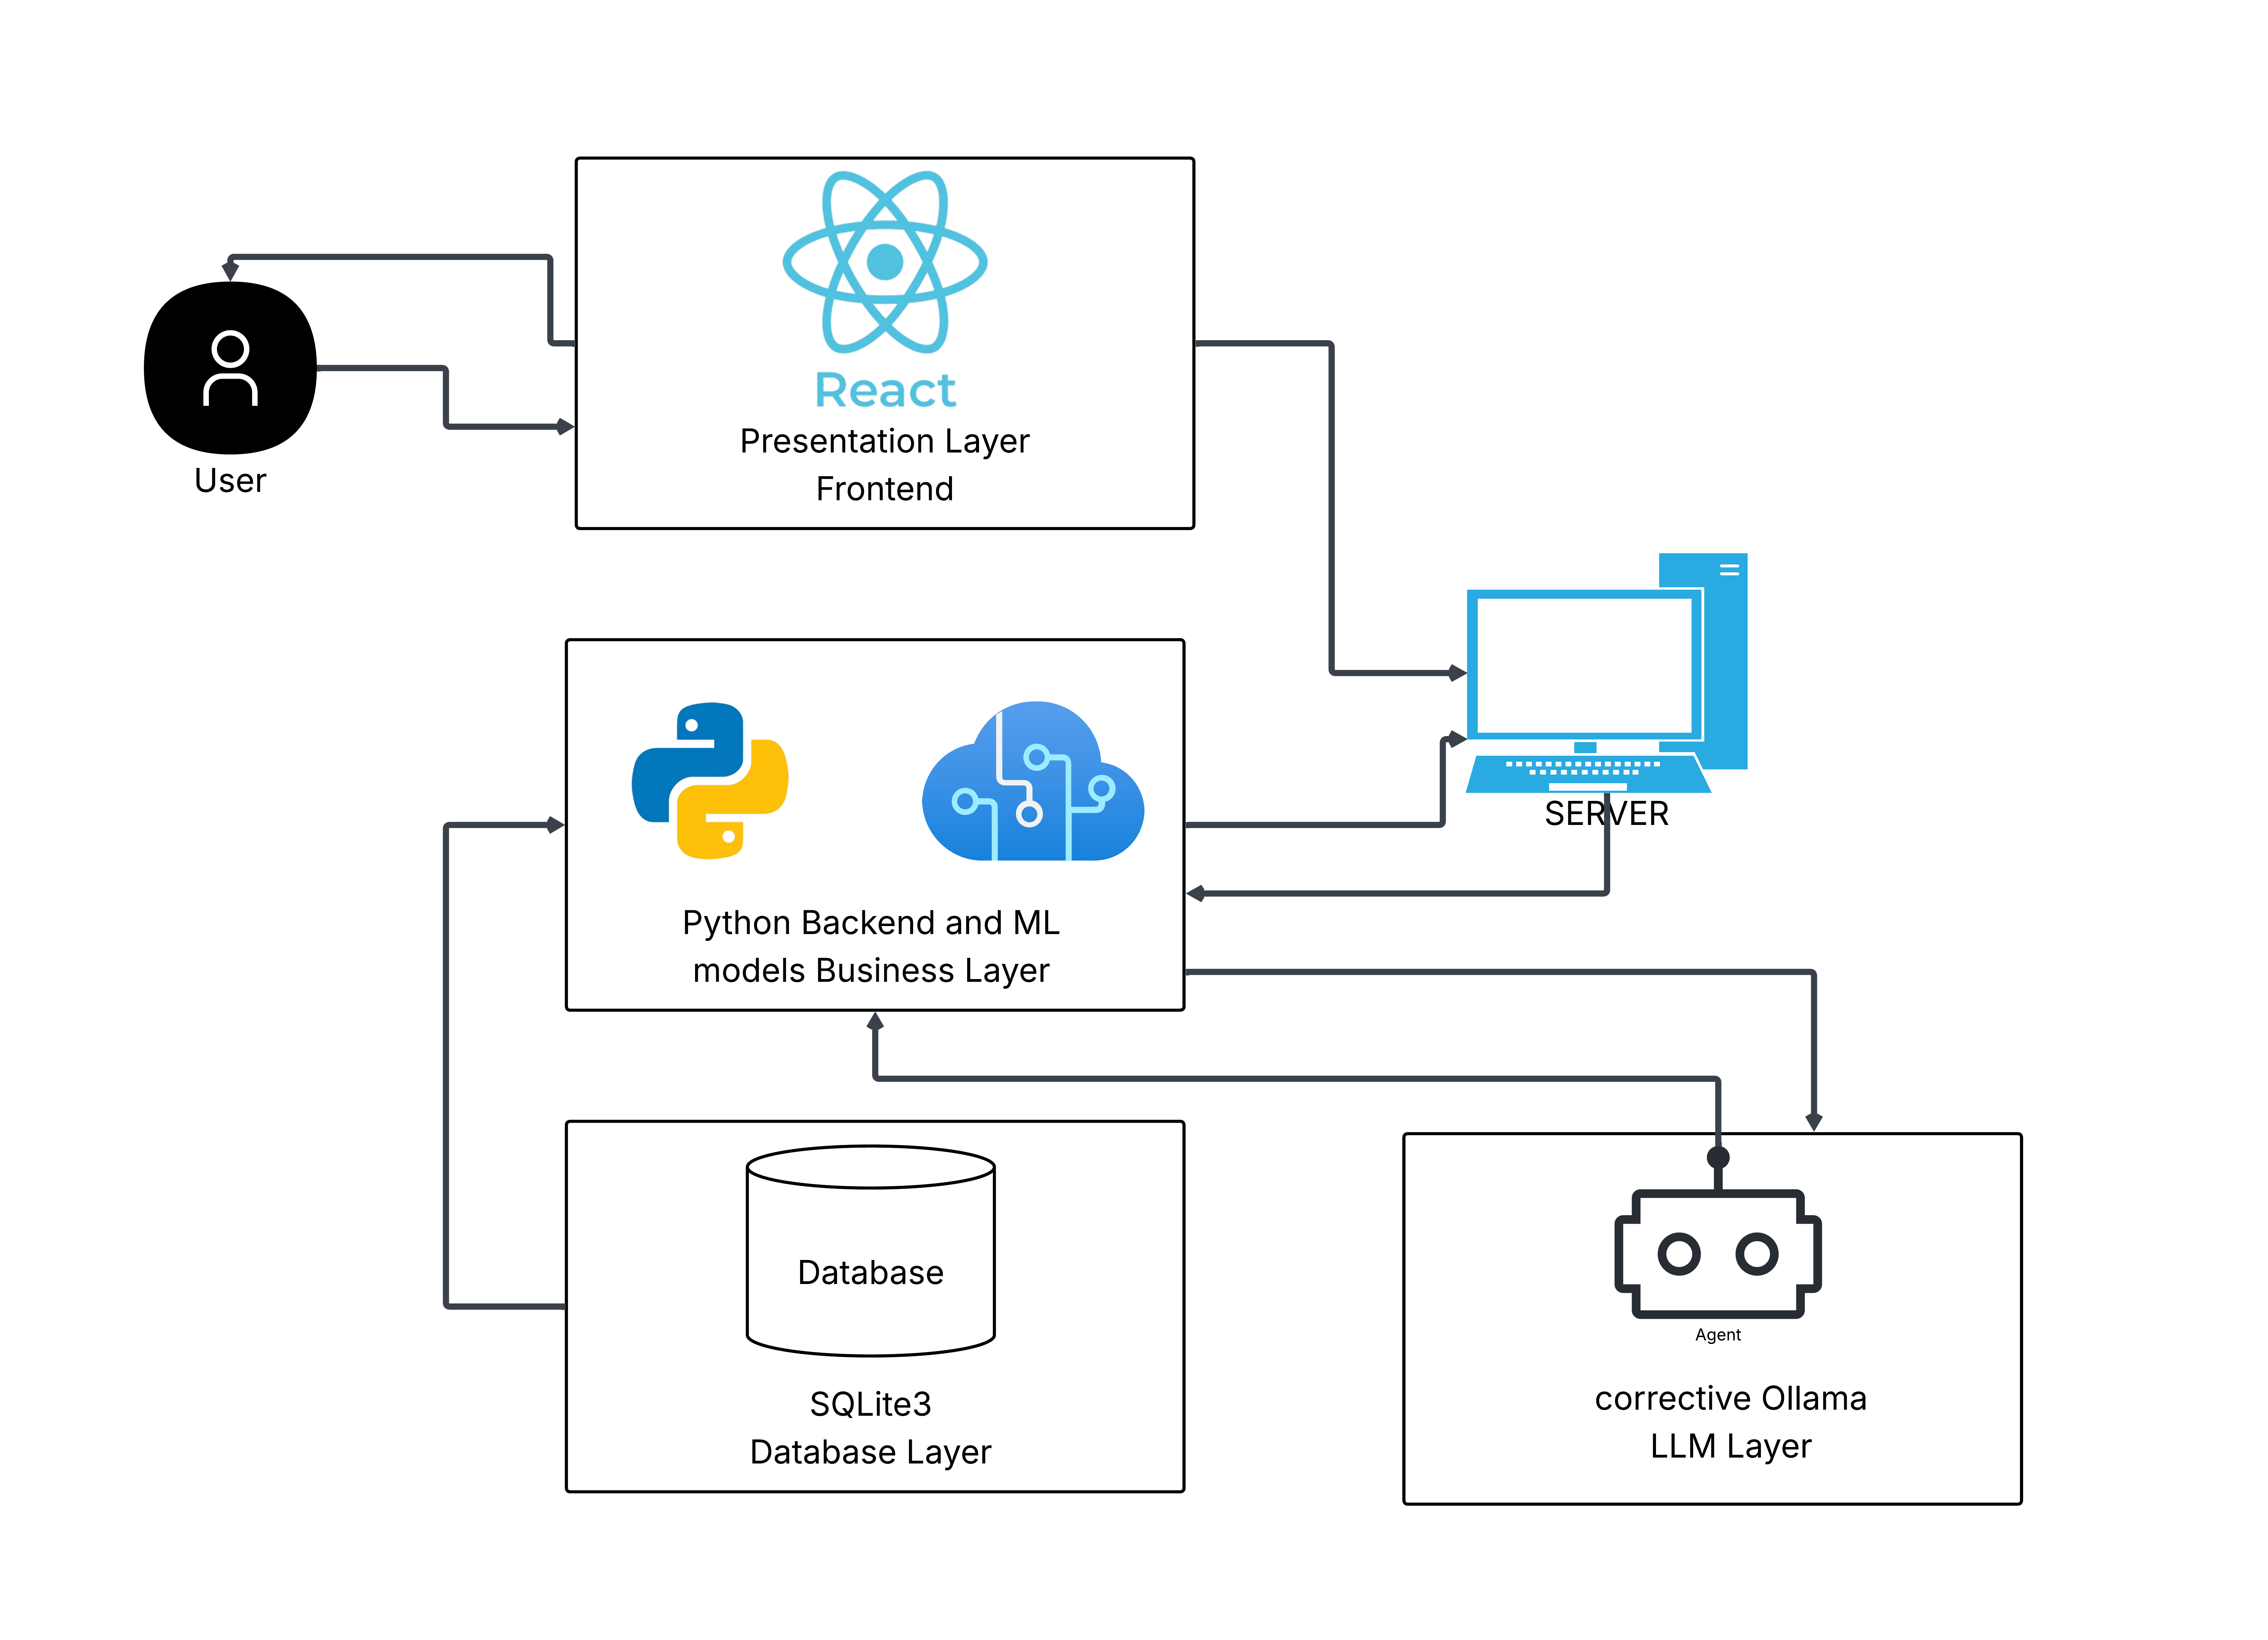
\includegraphics[width=\textwidth]{images/architecture.png}
    \caption{Architecture diagram of Silent Signals}
    \label{fig:architecture}
\end{figure}

\subsection{Subsystem Architecture}
The lip-reading module is the most complicated part of the entire software, so its subsystem is described in more detail here. It involves the use of the MediaPipe API \cite{googlemediapipe2026} for locating the face and cropping the mouth region from every frame of the LRW dataset \cite{ref:Chung:2016} during training, and from every frame of the user's video during use, and then processing the sequence of crops through a machine learning model. This model will then be used in the final project to determine the spoken words from the videos uploaded or streamed by the user. The subsystem therefore has three parts. The first is the pre-processing part, which reads frames, detects the 478 facial landmarks, smooths the mouth position and produces normalised mouth crops of a fixed size. The second is the model part, which takes a window of 29 crops and returns a probability for each word in the vocabulary. The third is the output part, which turns the probabilities into a predicted word with its confidence score and passes it to the corrective language model through the common model interface. Because the same pre-processing code is used for training and for live use, the model always receives input of the same form, which avoids a common source of errors when a trained model is deployed.

\subsection{Lip-Reading Model}
The lip-reading model, shown in Figure~\ref{fig:lipmodel}, begins with pre-processing that removes unnecessary information from the videos, followed by normalization for more stable training. The input then goes through a 3D CNN. A 3D network is used because the model not only needs to learn the two spatial dimensions of the shape of the lips but also how that shape changes over time, since predicting a word requires the full context of the movement, including the shapes that come before and after each frame. The convolution is applied in three layers of 32, 64 and 128 filters for the purpose of extracting features, the output of which is passed through a batch normalization layer and then through a ReLU activation function to introduce non-linearity. Following this, a three-dimensional max pooling layer reduces the size of the features. The pooled features are passed to a bidirectional LSTM, which reads the sequence both forwards and backwards so that each frame is interpreted in the context of the whole word. Finally, the output goes through a 0.5 dropout layer, which reduces overfitting to the training speakers, and a softmax layer, which gives the probability of each of the 500 words. The highest probability is the predicted word and its confidence score.

\begin{figure}[htbp]
    \centering
    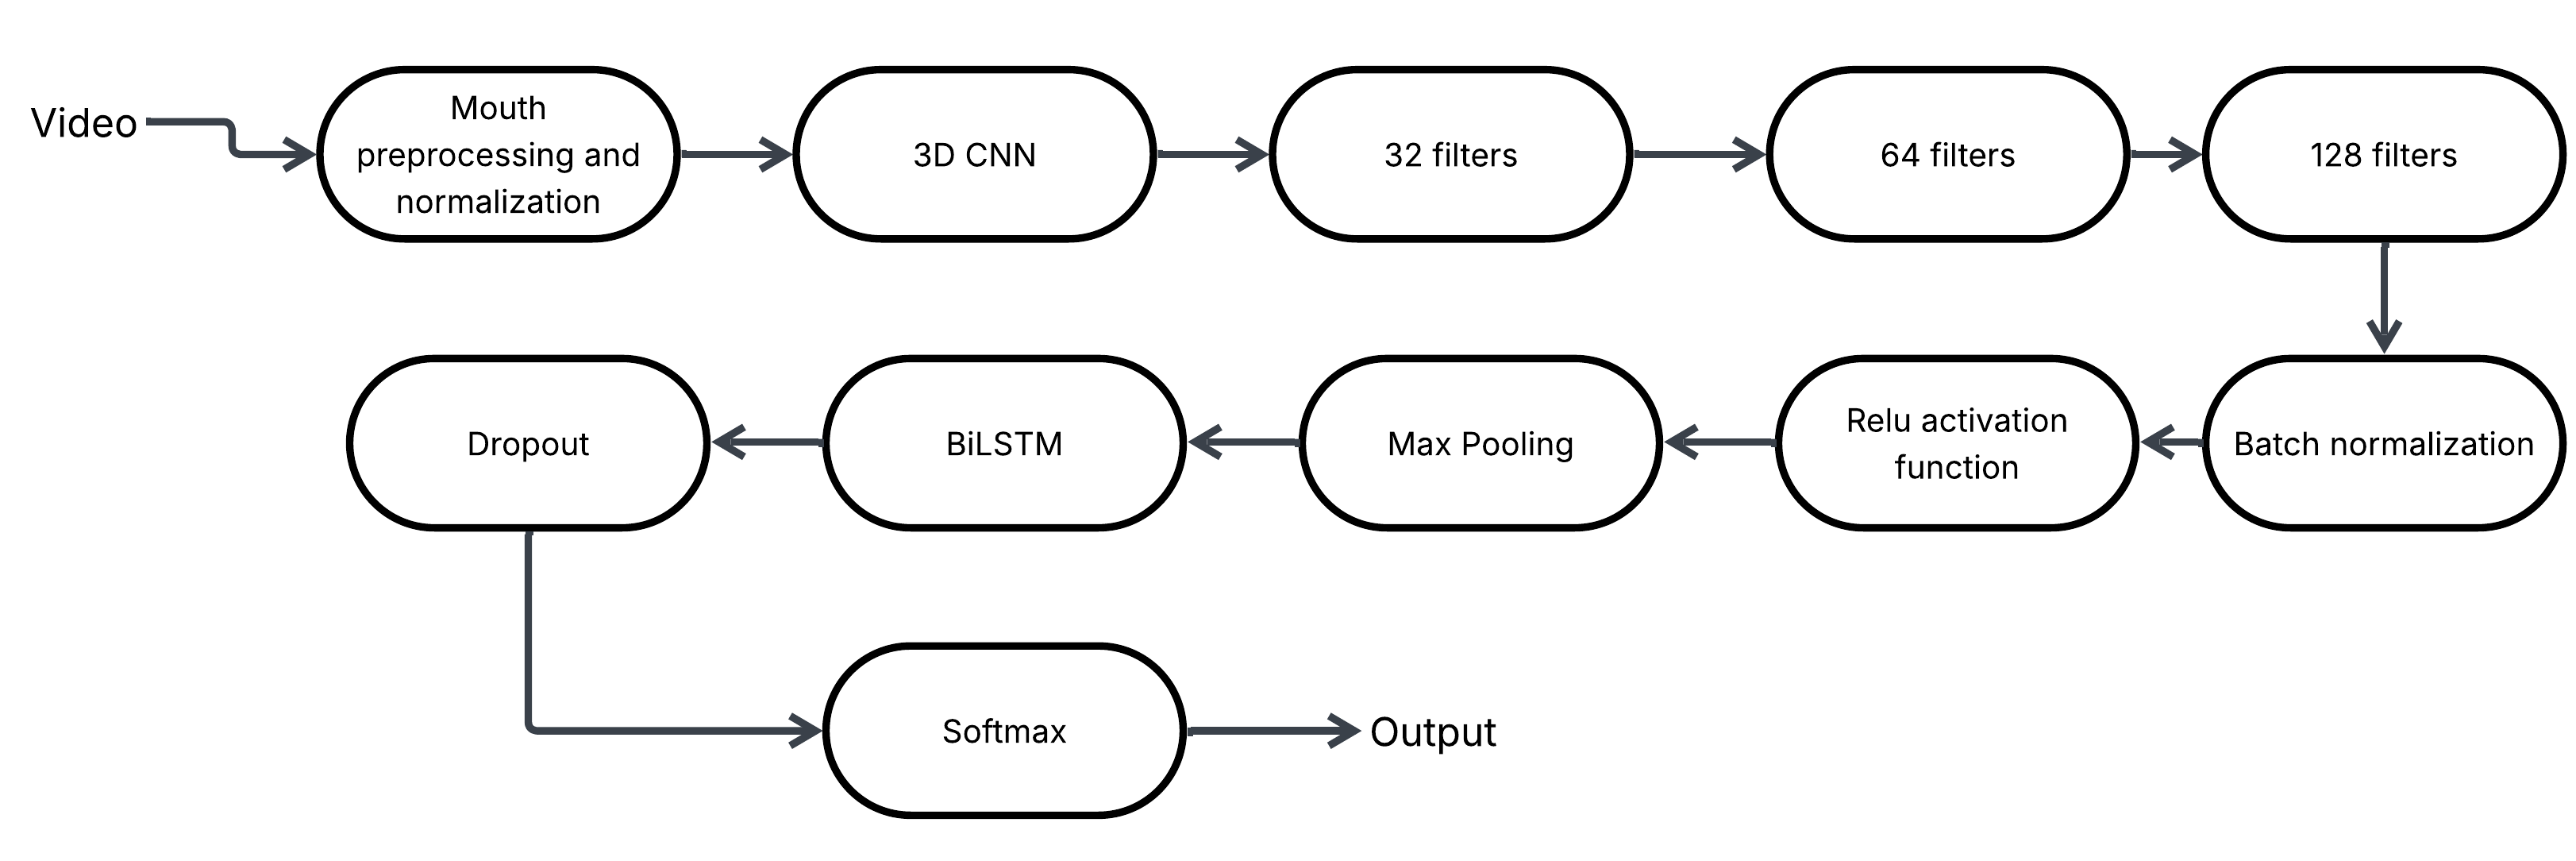
\includegraphics[width=\textwidth]{images/lip reading model architecture.png}
    \caption{Architecture of the lip-reading model}
    \label{fig:lipmodel}
\end{figure}

\section{Architectural Strategies}
The strategies we have chosen for the project are described in the subsections below, and together they determine the overall organisation of the system and its higher-level structures. Each strategy is a decision that affects more than one component, and each was taken with reference to the goals and guidelines stated earlier in this chapter. The first strategy concerns the choice of programming languages and frameworks for the frontend and the backend, which determines how the two halves of the system communicate and how the application reaches the user's phone. The second concerns the reuse of existing software components, which decides which parts of the system the team builds itself and which parts are taken from open source libraries and pretrained models, a decision that follows from the limited time and data available to the project. The third concerns data privacy and storage, which decides what happens to the videos and text that users send to the server and is the main way in which the privacy-centred design guideline is put into practice. For each strategy the subsection describes the decision and the reasoning behind it, so that a reader can see how the design goals were balanced against the constraints of the project and why other options were not chosen.

\subsection{Programming language}
For the frontend, we will be using React with npm and Expo for easy testing and deployment on Android devices. Expo allows the same React code to be run on a phone during development without building a native package each time, which makes it quick to test the interface on real devices. The backend will be made using Python 3.11 with the help of FastAPI and Uvicorn. Python was chosen because all the machine learning libraries used by the project, as well as the landmark detector and the language model runtime, provide Python interfaces, so the models and the server can live in one code base. This will enable us to create a simple and effective layered frontend and backend architecture. The backend and the frontend will communicate with one another using FastAPI endpoints and sockets hosted through Uvicorn: the networking will be handled by Uvicorn, which serves the application, and the API requests will be handled by FastAPI, which defines the endpoints and validates their inputs. The backend will be hosted on a desktop server which will host the lip-reading, sign language, text to speech and speech to text models as well as the corrective LLM through Ollama, so that all heavy processing takes place in one place with a GPU.

\subsection{Reuse of existing software components}
The reused components of the system involve the use of a pretrained model for the sign language detecting module, since public ASL data is too limited for the team to train a reliable recogniser from scratch within the project. In addition, there are also existing libraries which will be used to detect faces \cite{lugaresi2019mediapipe}, to crop the speaker's mouth \cite{googlemediapipe2026}, to detect emotions \cite{savchenko2022hsemotion}, and to train the lip-reading model \cite{tensorflow2015,paszke2019pytorch}. The corrective language model is also an existing model, Llama 3.2, run through Ollama \cite{ollama_llama32_3b}, rather than a model trained by the team. Reusing these components is a deliberate strategy. It follows the simplicity guideline and the time constraint, since building face detection, emotion recognition or a language model ourselves would consume the whole project without improving on published results, as the literature in Chapter~\ref{ch:lit} shows. It also keeps the cost of the system low, because all the reused components are open source. The team's own effort is therefore concentrated on the lip-reading model and on integrating the components into one application, which is where the project makes its contribution. Because every reused model is wrapped behind the common model interface, any of them can later be replaced by a better one without changing the rest of the system.

\subsection{Data privacy and storage}
The videos uploaded by the users will not be used for any training and will not be saved on the server. The only time they exist on the server will be during processing, after which they will be deleted immediately and will not be cached either. This will also apply to any intermediate output generated during the processing of the data, such as the cropped mouth regions, the landmark coordinates and the raw model predictions. The only information that is stored is the information listed in the database design of Chapter~\ref{ch:srs}, namely the user's account and settings, the registered guardians and emergency words, and the conversation history with the recognised text and detected emotion, which the user needs in order to review earlier conversations. This strategy follows from the privacy-centred design guideline and from the nature of the data, since a video of a person's face is sensitive personal information and the users of the system may be discussing private matters, for example with a doctor. Using a locally hosted language model for correction supports the same strategy, because the text of a conversation is never sent to an external service. Processing in memory also reduces the storage needed on the server, which keeps the hardware requirements and the cost of running the system low.

\section{Domain Model/Class Diagram}
The class diagram in Figure~\ref{fig:classdiagram} showcases an early prototype design of the classes and their interactions with each other, and the relationships of the classes are clearly shown. At the centre of the diagram is the Silent Signals class, which holds references to the User and handles all access to the database. The User class holds the user's identity, guardian details and emergency words, has a Guardian, holds a list of Conversation objects and is configured by a Settings object that stores the font size, dark mode and contrast preferences. The diagram contains two abstract classes, or interfaces, with their respective child classes. The first is the ML model interface, which defines a single run method that takes input bytes and returns a result; the lip-reading model, the text to speech model, the speech to text model and the sign language model all implement it, and their output is sent to the Corrective LLM class for post-processing before it is returned to the user. The second is the DB handler interface, which defines an update method and is implemented by separate handlers for settings, users, guardians and conversations. These two interfaces are what make the models and the database replaceable, which is one of the main goals of the design.

\begin{figure}[htbp]
    \centering
    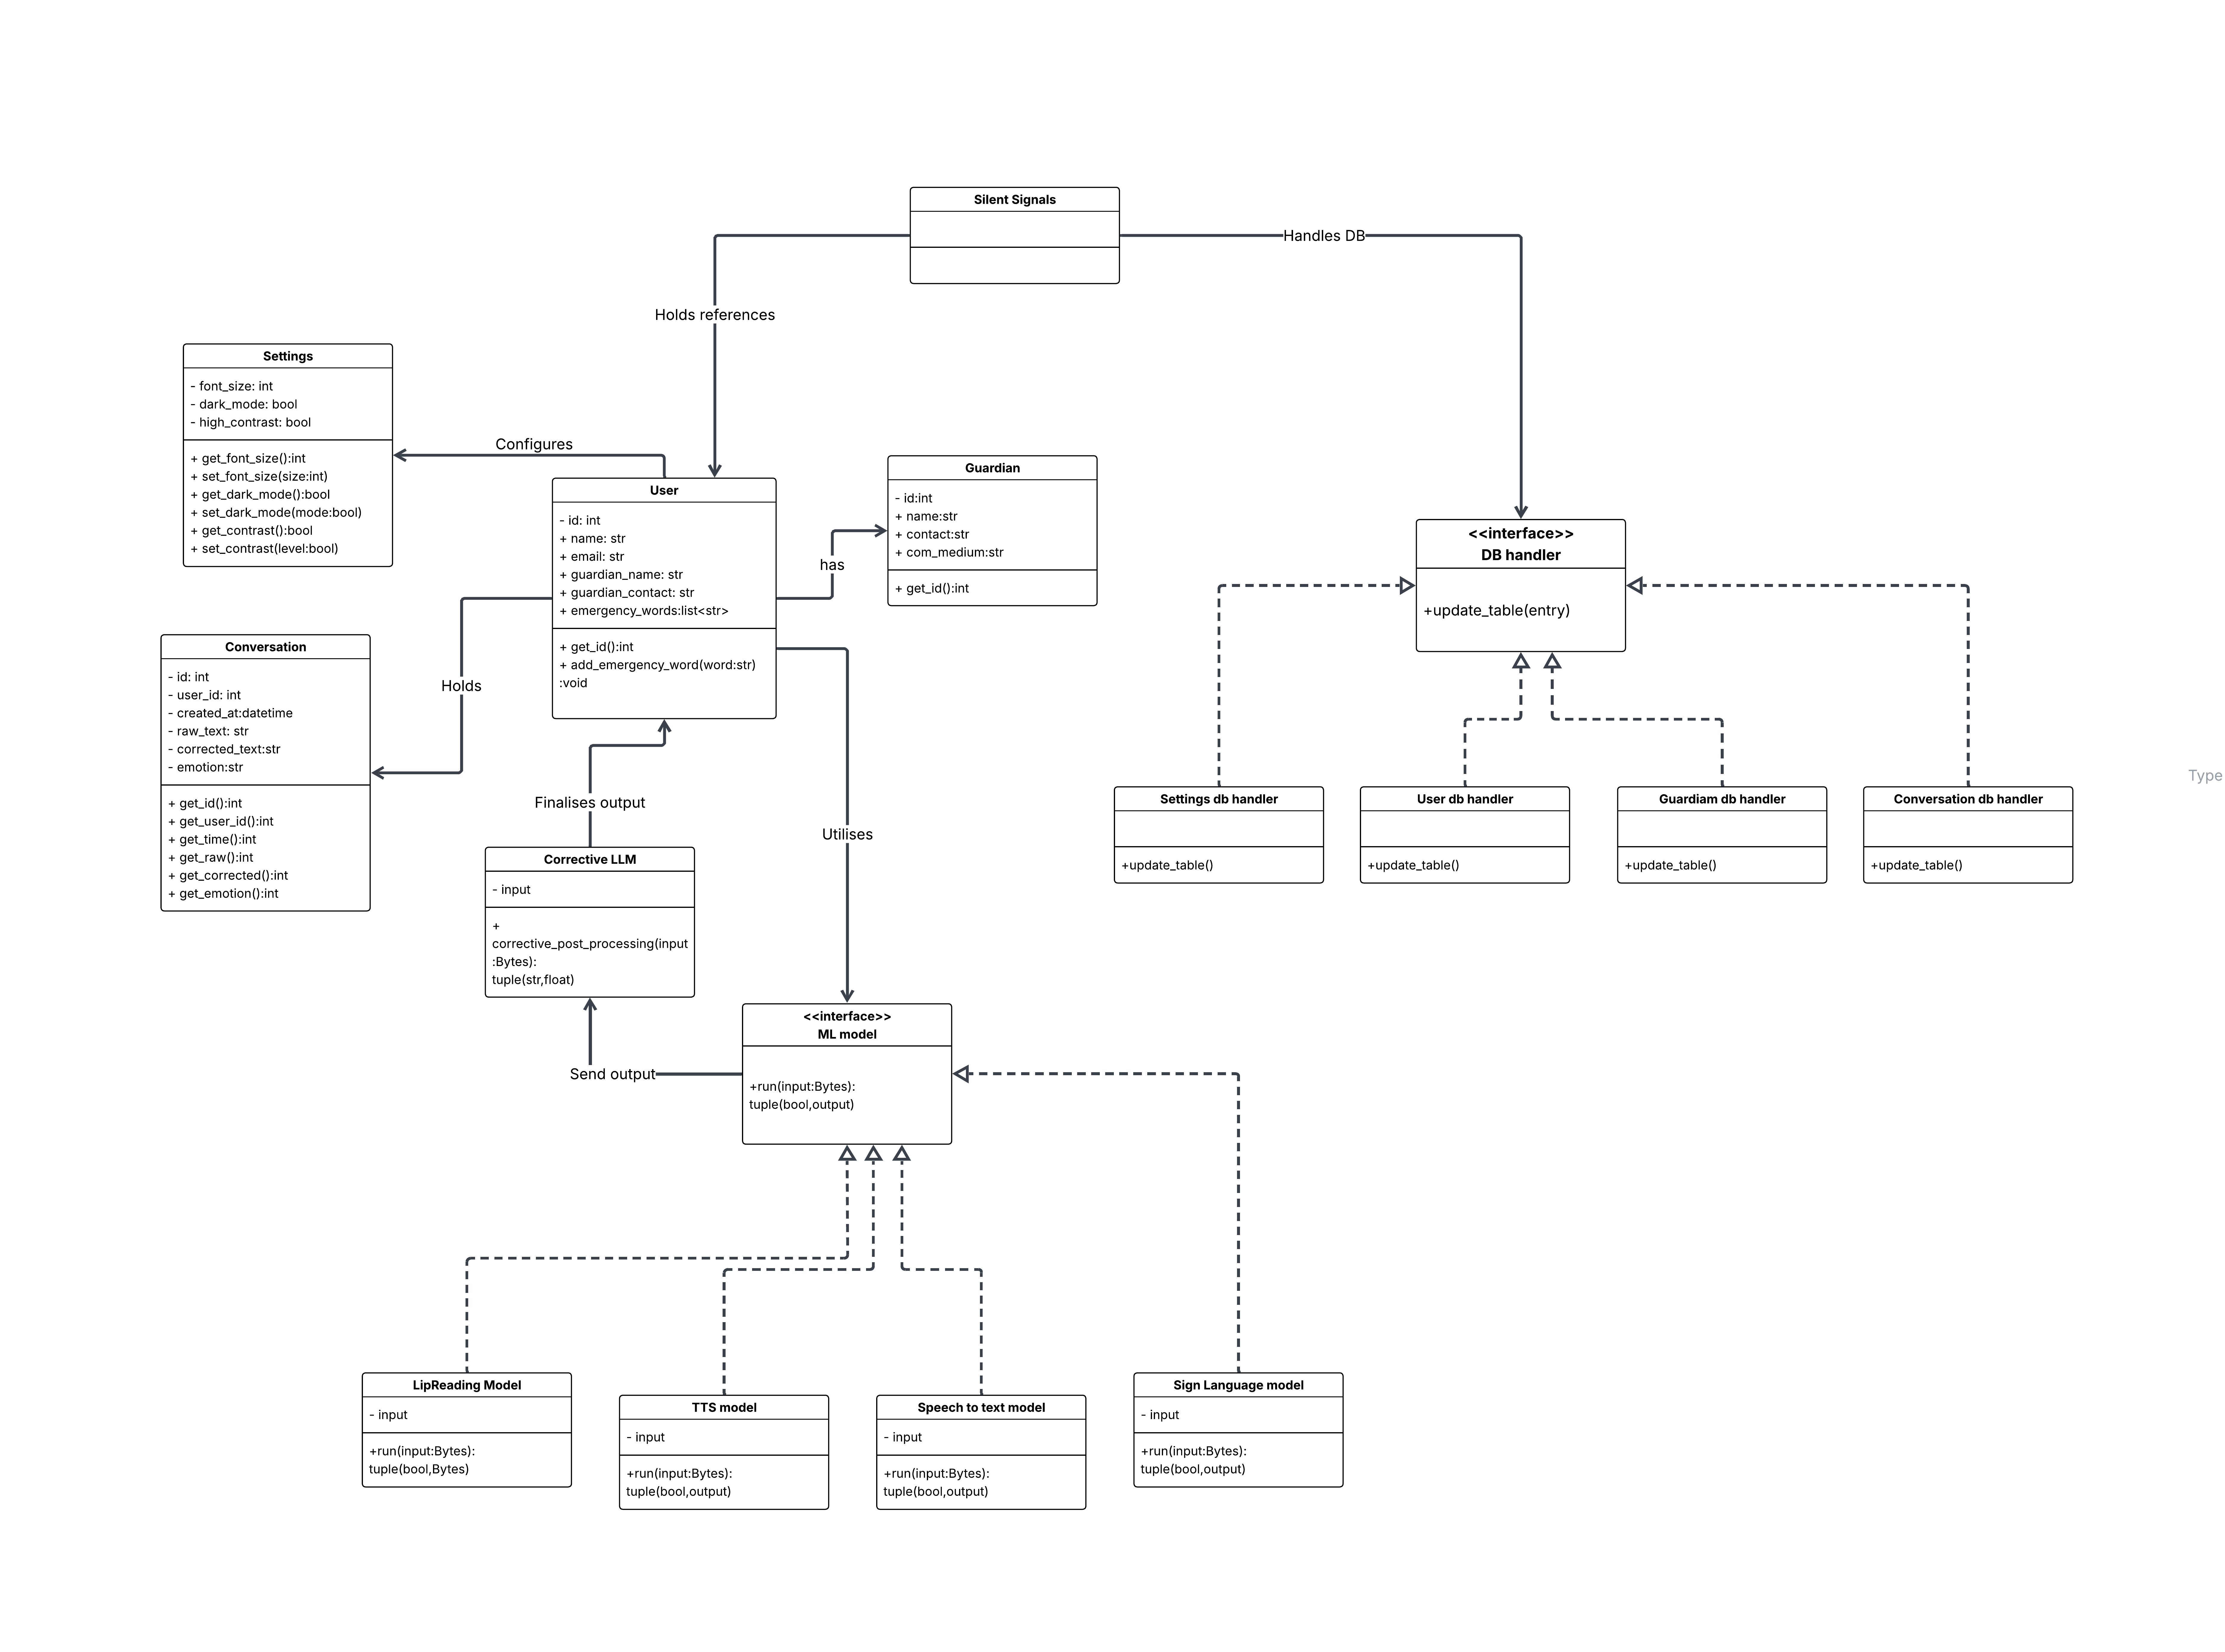
\includegraphics[width=\textwidth]{images/Silent Signals Class Diagram.png}
    \caption{Class diagram of Silent Signals}
    \label{fig:classdiagram}
\end{figure}

\section{Policies and Tactics}
The policies and tactics that will be followed in the project are described in the subsections below. Unlike the architectural strategies of the previous section, these decisions do not change the overall organisation of the system, but they affect the details of how it is implemented, maintained and used, and they help a team of three people to work on the same code base without getting in each other's way. The policies cover five areas. The organisation of the source code and its conventions decides where each part of the system lives and how the folders are structured. The user interface policy sets the principles that every screen must follow, with particular attention to accessibility. The modularity policy describes how object-oriented design and polymorphism are used to keep components independent of each other. The library management policy explains how the Python dependencies are recorded so that every development machine and the server use the same versions. Finally, the version control policy describes how changes to the code and to this report are tracked and shared. Each policy is chosen to support the goals of replaceability, simplicity and privacy stated earlier, and each is simple enough to be followed consistently for the whole length of the project.

\subsection{Source code organization and conventions}
The code of the project will be divided into separate frontend and backend folders, so that the two halves of the system can be developed, run and tested independently. The frontend will comprise the React application of the system along with the Expo configuration used to run it on Android devices, with the screens, shared components and the code that calls the backend kept in their own subfolders. The backend will consist of a Python environment together with the libraries installed on each of our development machines, and its individual components will also be kept in their respective folders, such as the models, the core components of the server, the database handlers and the training data and scripts. Keeping the models in their own folder, with one subfolder per model, matches the class diagram, in which each model is a separate class behind a common interface, and it means that adding or replacing a model only touches one folder. Training scripts and data are kept apart from the code that runs on the server, so that large datasets are never deployed by accident.

\subsection{User Interface}
The user interface will be simple and easy to use, because the primary users of Silent Signals may have difficulty with small text, low contrast or complex navigation, and because many of them will use the application in stressful situations such as a hospital visit or an emergency. Every main screen will be reachable from the home screen in one step, buttons will be large with short labels, and the emergency phrases will be visible at all times. The interface will offer accessibility settings for easier viewing by people with disabilities, namely adjustable font size, dark mode and a high contrast mode, and these settings will be stored in the user's profile so that they are applied automatically each time the user logs in. At the same time, the interface will use a colour scheme that appeals to the vast majority of people, so that the application does not feel like a specialised medical tool and is pleasant for the hearing partner to look at as well. The same layout will be used for the lip-reading and the sign language screens, so that a user who switches between the two modes does not have to learn a second interface. The aim is an interface that a first-time user can learn without training, as required in Chapter~\ref{ch:srs}.

\subsection{Modularity}
The different modules of the system will use modularity and polymorphism within an object-oriented design. This is to avoid any hard coding and to avoid being unable to add further features or to change the machine learning models that we will be implementing. In practice, each model is a class that implements the common ML model interface shown in the class diagram, with one run method that accepts the input and returns the result, and each database table is accessed through a handler class that implements the common DB handler interface. The rest of the backend only calls these interfaces and never depends on the details of a particular model or table. As a result, a model can be retrained, replaced by a newer architecture from the literature, or swapped for a lighter version for slower hardware, simply by writing a new class that implements the interface and changing the configuration that selects it. The same applies to the database, which could be moved from SQLite3 to a larger database system later without changing the code that uses it. This policy is the practical form of the replaceability goal, and it also makes testing easier, because each model or handler can be tested on its own with fixed inputs before it is connected to the rest of the system.

\subsection{Library management}
All the required libraries for the Python backend will be listed in a requirements.txt file that pip, the Python package manager, will read in order to install them on each of our machines, which makes it easy to keep track of the libraries used and to set up a new machine quickly. Each library in the file will be given with a specific version, so that every member of the team and the server use the same versions and a model trained on one machine behaves the same way on another. This matters for a project of this kind, because deep learning and landmark detection libraries change often, and a difference in versions can change the output of a model or break code that worked before. When a new library is needed, the developer who adds it will also add it to the file in the same change, so that the file always matches the code. The backend will be run inside a virtual environment created from this file, which keeps the project's libraries separate from anything else installed on the machine.

\subsection{Version control}
We will be using Git for version control of the source code, and GitHub for hosting the source code so that every member of the team works from the same shared repository. Every change to the code is recorded as a commit with a short message that describes it, which gives a full history of the project and makes it possible to go back to an earlier version if a change breaks something. Before starting work, each member pulls the latest changes from the repository, and after finishing a piece of work they commit and push it, so that the others receive it promptly. Larger features, such as a new model or a new screen, can be developed on a separate branch and merged into the main branch once they work, which keeps the main branch in a usable state at all times. The same repository also holds this report, written in LaTeX, so that the code and its documentation stay together and their history is recorded in the same way. Files that are generated automatically, such as build outputs, temporary files and large datasets, are excluded from the repository so that it stays small and every clone works on every operating system used by the team. This policy supports the Scrum method, since the work of each sprint can be reviewed directly from the commit history.

\section{Conclusion}
This chapter has presented the design of Silent Signals. The system is organised as a layered architecture with a React frontend on the user's phone, a Python backend with FastAPI and the machine learning models on a central server, an SQLite3 database layer and a corrective language model layer run through Ollama. The design considerations recorded the assumptions and dependencies of the system, the constraints of accuracy, privacy, network and hardware under which it works, the goals of replaceability, simplicity, privacy, accuracy and throughput, and the Scrum method used by the team. The lip-reading subsystem was described in detail as a pipeline of landmark-based pre-processing, a 3D CNN and BiLSTM model and an output stage that returns words with confidence scores. The architectural strategies explained the choice of languages and frameworks, the reuse of pretrained models and open source libraries for everything except the lip-reading model, and the policy of processing user videos in memory and never storing them. The class diagram showed how two abstract interfaces, one for the models and one for the database handlers, make every model and table replaceable. The policies and tactics fixed the organisation of the source code, the principles of the user interface, the use of modularity, the management of libraries and the use of version control for both the code and this report.

% \chapter{Implementation and Test Cases}
% \label{ch:impl}
% For each chapter, provide a paragraph of introduction and at the end, a paragraph of conclusions. (Not the programming code but the algorithmic and procedural details especially related to the hidden/ backend algorithms that are not covered in the design)
% \section{Implementation}
% Whatever implementation that you have done so far, please elaborate here.
% Give clear details of the algorithms that were implemented along with the platform and the APIs which were used. 
% \textcolor{red}{NOTE: For FYP-1, this chapter can be changed to description of prototype developed.}
% \subsection{Implementation of First Component/Algorithm}
% Write the implementation of the first component of your system here.
% \section{Test case Design and description}
% \textcolor{red}{This section will be added in FYP-II.} Summarize the common attributes of test cases. This may include input constraints that must be true for every input in the set of associated test cases, any shared environmental needs, any shared special procedural requirements, and any shared case dependencies. The following scheme is recommended for describing test cases in detail. The Sample test case is provided in table \ref{tab:3}.
% \begin{table}[!ht]
% \caption{Sample Test case No.1}

% \centering
% \begin{tabular}{|llll|}
% \hline
% \multicolumn{4}{|c|}{\textbf{\textless{}Software Component Name\textgreater{}}} \\ \hline
% \multicolumn{4}{|c|}{\textbf{\textless{}Reference\textgreater{}}} \\ \hline
% \multicolumn{1}{|l|}{\textbf{Test Case ID:}} &
%   \multicolumn{1}{l|}{\textit{Reference Number}} &
%   \multicolumn{1}{l|}{\textbf{QA Test Engineer:}} &
%   \textit{Name of personnel} \\ \hline
% \multicolumn{1}{|l|}{\textbf{Test case Version:}} &
%   \multicolumn{1}{l|}{\textit{Version number}} &
%   \multicolumn{1}{l|}{\textbf{Reviewed By:}} &
%   \textit{Testing Team lead} \\ \hline
% \multicolumn{1}{|l|}{\textbf{Test Date:}} &
%   \multicolumn{1}{l|}{\textit{Date}} &
%   \multicolumn{1}{l|}{\textbf{\begin{tabular}[c]{@{}l@{}}Use Case \\ Reference(s):\end{tabular}}} &
%   \textit{Relation to use cases} \\ \hline
% \multicolumn{1}{|l|}{\textbf{Revision History:}} &
%   \multicolumn{3}{l|}{\textit{Refer to previous test   case identity (if any)}} \\ \hline
% \multicolumn{1}{|l|}{\textbf{Objective:}} &
%   \multicolumn{3}{l|}{\textit{Need and   scope of the testing}} \\ \hline
% \multicolumn{1}{|l|}{\textbf{\begin{tabular}[c]{@{}l@{}}Product/Ver/\\ Module:\end{tabular}}} &
%   \multicolumn{3}{l|}{\textit{Refer to overall system being built and the place of this test case in it.}} \\ \hline
% \multicolumn{1}{|l|}{\textbf{Environment:}} &
%   \multicolumn{3}{l|}{\textit{Necessary and desired properties of the test environment.}} \\ \hline
% \multicolumn{1}{|l|}{\textbf{Assumptions:}} &
%   \multicolumn{3}{l|}{\textit{Assumptions that might affect the testing process.}} \\ \hline
% \multicolumn{1}{|l|}{\textbf{Pre-Requisite:}} &
%   \multicolumn{3}{l|}{\textit{Necessary condition that  needs to be fulfilled before the test case.}} \\ \hline
% \multicolumn{1}{|l|}{\textbf{Step No.}} &
%   \multicolumn{1}{l|}{\textbf{Execution   description}} &
%   \multicolumn{2}{l|}{\textbf{Procedure result}} \\ \hline
% \multicolumn{1}{|l|}{} &
%   \multicolumn{1}{l|}{\textit{Events being tested.}} &
%   \multicolumn{2}{l|}{\textit{Mention software response.}} \\ \hline
% \multicolumn{4}{|l|}{\textbf{Comments:}} \\ \hline
% \multicolumn{4}{|c|}{\textbf{Passed      Failed     Not Executed}} \\ \hline
% \end{tabular}
% \label{tab:3}
% \end{table}
% \section{Test Metrics}
% Summarize here the common ground of attributes of test case metrics as explained in Table \ref{tab:4}.
% \begin{table}[!ht]
% \centering
% \caption{Sample Test case Matric.No.1}

% \begin{tabular}{|l|l|}
% \hline
% \textbf{Metric}                      & \textbf{Purpose}                                                                                                        \\ \hline
% \textbf{Number of Test Cases}        & \begin{tabular}[c]{@{}l@{}}Total number of test cases that you have\\ developed for  your system.\end{tabular}          \\ \hline
% \textbf{Number of Test Cases Passed} & The number of test cases that successfully passed                                                                       \\ \hline
% \textbf{Number of Test Cases Failed} & The number of test cases that failed                                                                                    \\ \hline
% \textbf{Test Case Defect Density}    & \begin{tabular}[c]{@{}l@{}}(No of test cases failed * 100) \\ No of test cases executed\end{tabular}                    \\ \hline
% \textbf{Test Case Effectiveness}     & \begin{tabular}[c]{@{}l@{}}No of defects detected using test cases *100\\ Total number of defects detected\end{tabular} \\ \hline
% \textbf{Traceability Matrix} &
%   \begin{tabular}[c]{@{}l@{}}Traceability is the ability to determine that each\\  the feature has a source in requirements and each \\ requirement has a corresponding implemented feature.\end{tabular} \\ \hline
% \end{tabular}
% \label{tab:4}
% \end{table}
% \subsection{Sample Test case Metric.No.2}
% Similar to the above table, add here for test metrics 2,3,4.\\
% \chapter{User Manual}
% \textcolor{red}{This chapter will be added in FYP-II.} Design a complete user manual of your application and add that in this chapter.
% \textcolor{red}{NOTE: This Chapter is optional for Research projects but compulsory for Development projects.}\\
% \chapter{Experimental Results and Discussion}
% This chapter will be added in FYP-II. Give proper analysis and discussion of experimental results (in plain English text) along with tables of results.  For each chapter provide a paragraph of introduction and in the end a paragraph of conclusions.\\
% \textcolor{red}{NOTE: This Chapter is optional for Development projects but compulsory for Research projects.}

% \chapter{Conclusions}
% \label{ch:concl}
% \section{aa}
% \subsection{dfs}
% \subsubsection{dsd}
% {\bf This chapter is mandatory}.  
% Give conclusions and summary of the work done.  What were your findings and what were the results?  Discuss in detail whether the scope of your project was entirely covered or not and whether the objectives of the project were met or not.  What challenges did you face and what has been left out and why.\\
% Sum up all the conclusions of all the chapters here to make a final conclusion chapter.  Do not repeat any text, just summarize it in different words. Give recommendations for future work also.\\
% \textbf{For FYP-1 it is mandatory to list down a plan of the work to be done for FYP-2.}

{
\bibliographystyle{ieeetr}
\bibliography{fypbib} %specify your .bib file here
}
% %ADD APPENDICES IF REQUIRED OTHERWISE COMMENT IT OUT
% \appendix
% \chapter{First Appendix if Required}
% If you want to add appendices then make sure you provide a proper title.  Add different appendices by using the chapter command as shown for this one.  They will automatically be added to the table of contents.

% \section{References}
% See how .bib file is prepared.  The bibliography would be automatically added by Latex.  So here is how you cite papers (you'll need to view the .bib file to understand).  \cite{ref:Duda:2000} is the correct way to make one citation and \cite{ref:Bishop:2006,ref:SVMGuide} to make multiple citations. You can see various reference styles for manuals \cite{ref:SVMGuide}, conferences \cite{ref:guyon:2007}, websites \cite{ref:IJCNNChallenge:2007} and journal articles \cite{ref:guyon:2007a}.  Also, note that all citations appear in the order in which they appear within text.  They are not sorted according to author names.

% \section{Equations}
% Make sure you use the math environment for writing equations.  Again, make sure you do not hard code equation numbers.  Use label and ref commands of Latex to number them and reference them.  Here is an example of (\ref{eq:energy})
% \begin{equation}\label{eq:energy}
% E = mc^2
% \end{equation}
% Note, how the equation is referenced by its equation number within brackets.  

% \section{Figures}
% To insert a figure, you can use the following code as template.  Here the figure is referenced using ref command of Latex.  So Figure \ref{fig:fast} is the FAST logo.  DO NOT HARD CODE FIGURE NUMBERS.  Let Latex manage them for you.

% \begin{figure}[!hbt]
% \centering
% 
\includegraphics[width=1in]{Figures/fastlogo.png}
% {\caption {\label{fig:fast}{\textbf{Fast Logo is the Caption.}}}}  
% \end{figure}

% \section{Tables}
% Note how tables can be added in Latex.  Also, make sure you use label and ref commands to define and use table numbers.  You can use Table \ref{tbl:SomeTable} as a template to make tables, add captions to them and reference them.  DO NOT HARD CODE TABLE NUMBERS.  Let Latex manage their numbering for you.

% If you are having problems in managing Latex tables, you may use Lyx \url{https://www.lyx.org/}. 


% \begin{table}[hbt]

% \begin{center}
% \caption{\label{tbl:SomeTable} \textbf{Give a Caption to the Table.}}
% \begin{tabular}{|l|c|c|} 
% \hline
% \textbf{No.}&\textbf{Column 1}&\textbf{Column 2}\\
% \hline
% 1.&Some data&More data\\
% \hline
% 2.&Some values&More values\\
% \hline
% \end {tabular}

% \end{center}

% \end{table}

% \section{Pseudo Code}
% When you need to explain an existing algorithm of an algorithm you devised, then you should use pseudo code notation. Given below, algorithm  \ref{algo:one}, is an example. Note how the numbering is managed by the Latex itself.

% \begin{algorithm}[H]
%  \KwData{this text}
%  \KwResult{how to write algorithm with \LaTeX2e }
%  initialization\;
%  \While{not at end of this document}{
%   read current\;
%   \eIf{understand}{
%    go to next section\;
%    current section becomes this one\;
%    }{
%    go back to the beginning of current section\;
%   }
%  }
%  \caption{How to write algorithms}
%  \label{algo:one}
% \end{algorithm}

% \section{Code of Programming Languages}
% If you need to add C++, Java or any other programming language's code, then you can use ``listings'' package. Following is an example. Normally, the code is only added in the appendices to avoid clutter in the document.

% \begin{lstlisting}

% #include <stdio.h>
% #define N 10
% /* Block
%  * comment */

% int main()
% {
%     int i;

%     // Line comment.
%     puts("Hello world!");
    
%     for (i = 0; i < N; i++)
%     {
%         puts("LaTeX is also great for programmers!");
%     }

%     return 0;
% }
% \end{lstlisting}

% \section{Recommendations for \LaTeX}
% Here we are providing you with only two Latex source files.  main.tex and fypbib.bib file. You can also start a project at \url{overleaf.com} and upload the zip file of this template there and share the Latex source between your group and supervisor.  This way all of you can work on the Latex files together online.


\end{document}


